\section{Simulationen}

Die Simulationen sollen Kenntnisse und erste Einblicke bezüglich der beiden Steuerungsverfahren der Phasenanschnitt- sowie Schwingungspaketsteuerung liefern. Dazu werden die beiden Verfahren sowohl mit Plecs als auch in Matlab simuliert und die Resultate auf ihre Richtigkeit geprüft. Zuerst wird auf die Simulation mit Matlab eingegangen, danach diejenigen mit Plecs erläutert.

\subsection{Simulation mit Matlab}\label{sec:Simulation_mit_Matlab}
Um die einphasigen Plecs-Simulationen der Phasenanschnitt- und Schwingungspaketsteuerung zu verifizieren, errechnete man parallel zu den Plecs-Simulationen die gleichen Verfahren mit Matlab durch. Im folgenden Abschnitt ist aufgezeigt, wie die Ergebnisse der Matlabfunktionen zustande gekommen sind und welche Überlegungen zu den verschiedenen Ansteuerungsarten vorgenommen wurden. Die verwendeten Berechnungen des Amplituden- und Phasenspektren sind im Kapitel \ref{sec:Verzerrte_Schwingung} ersichtlich.

\subsubsection{Einphasige Phasenanschnittsteuerung mit 60\textdegree\hspace{0.02cm} und 90\textdegree}
Als Erstes simulierte man eine periodische Sinusfunktion im Zeitbereich mit verschiedenen Phasenanschnittswinkeln. Die Periodenlänge ist definiert auf 2$\pi$. Die Amplitude des Sinus wurde auf eins normiert. Der Winkel des Phasenanschnittes wurde mit verschiedenen, geläufigen Werten wie zum Beispiel 30\textdegree, 45\textdegree \hspace{0.02cm}, 60\textdegree \hspace{0.02cm}, 90\textdegree \hspace{0.02cm} oder 120\textdegree \hspace{0.02cm} betrachtet. In Abbildung \ref{fig:Einganssignal_60} erkennt man die Sinusfunktion mit einem Phasenanschnitt von 60\textdegree \hspace{0.02cm} und in der Abbildung \ref{fig:Einganssignal_90} einen mit 90\textdegree \hspace{0.02cm}. Weitere Funktionen mit anderen Anschnittswinkeln sind im Anhang im Kapitel \ref{sec:Vergleich_der_Resultate} ersichtlich.

 

\begin{figure}[h]
	\centering
	\subfloat[][]{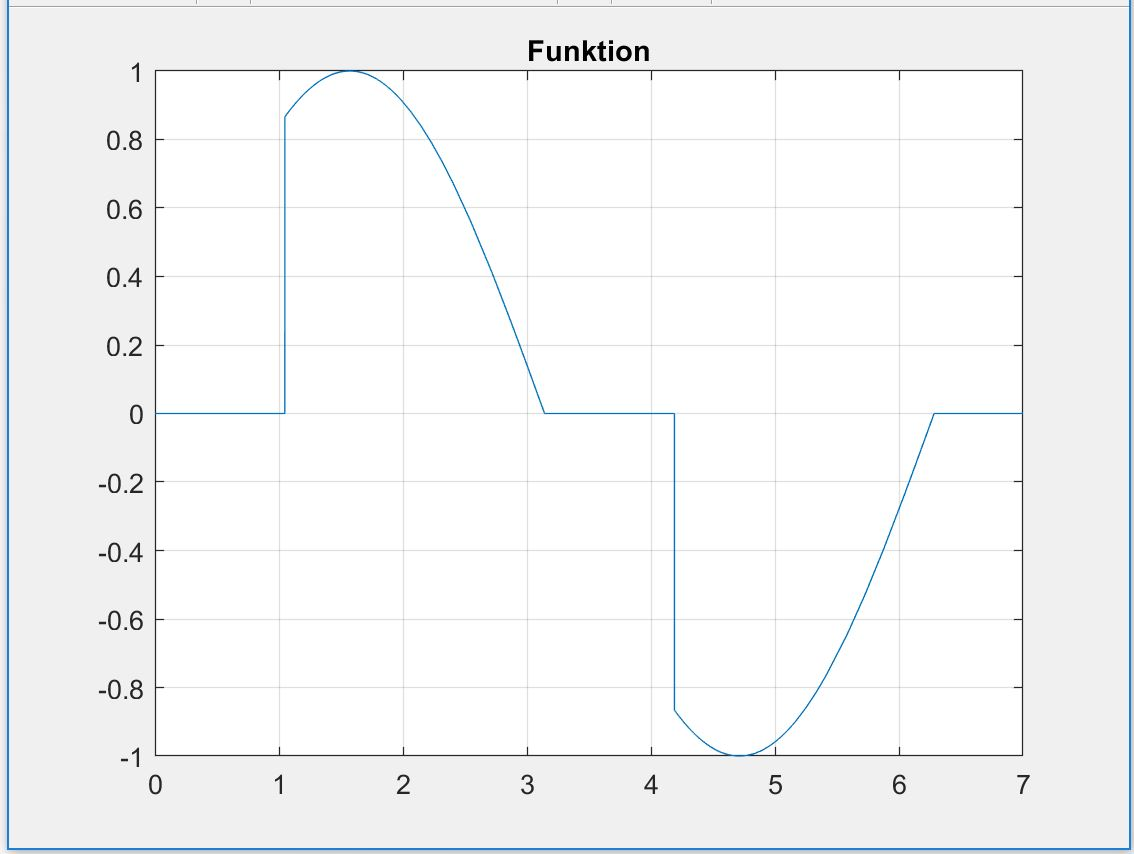
\includegraphics[width=0.47\linewidth]{eingangssignal_60.png}\label{fig:Einganssignal_60}}\qquad
	\subfloat[][]{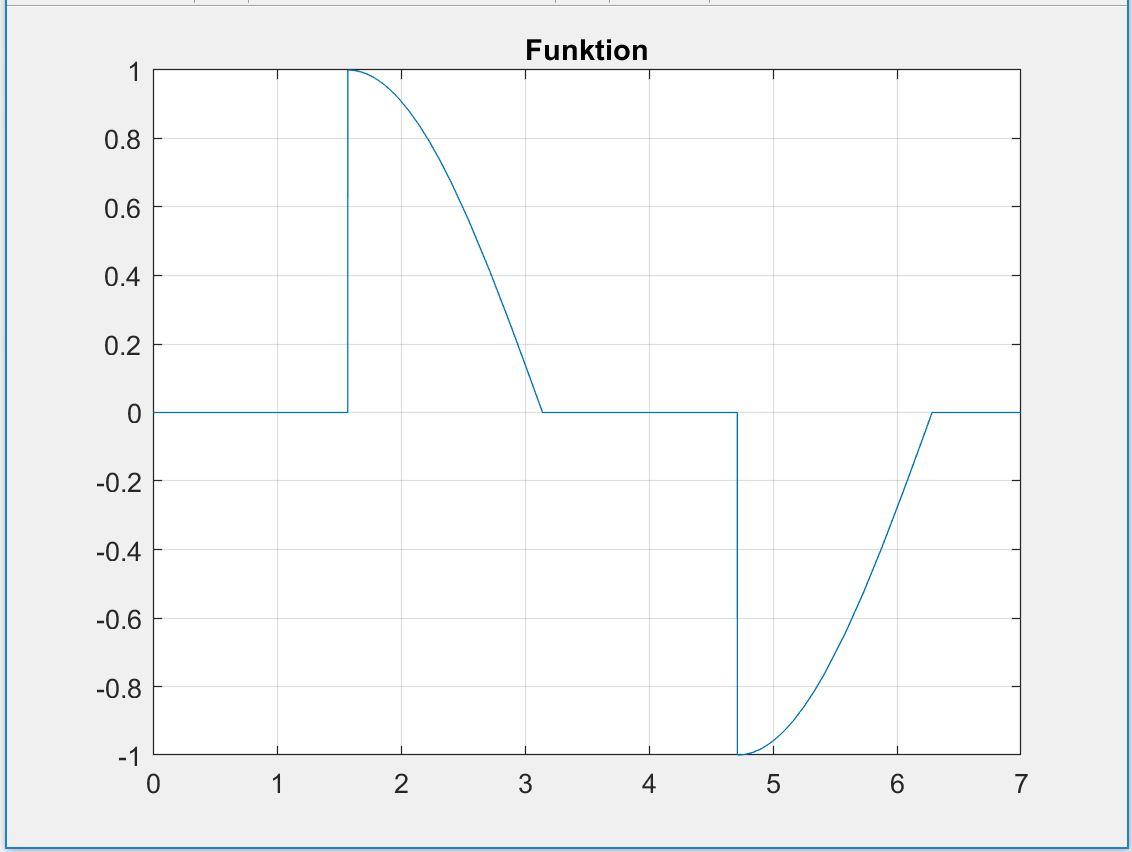
\includegraphics[width=0.47\linewidth]{eingangssignal_90.png}\label{fig:Einganssignal_90}}
	\caption{Einganssignal mit Phasenanschnitt (a) $60^\circ$ (b) $90^\circ$}
	\label{fig:eingangssignal_mit_Matlab}
\end{figure} 

Nachdem man die Funktion konstruiert hat, wird diese in die einzelnen Frequenzanteile zerlegt. Man bezeichnet dies als Fourier-Analyse. Gemäss Formel \ref{a0}, \ref{an} und \ref{bn} konnten die Fourier-Koeffizienten $a\textsubscript{0}$, $a\textsubscript{n}$ und $b\textsubscript{n}$ berechnet werden. Anschliessend wurden das Amplituden- und Phasenspektrum mit den Formeln \ref{Amplitudenspektrum} und \ref{Phasenspektrum} bestimmt.
\newpage
Die Darstellung im Zeitbereich beziehungsweise im Frequenzbereich sind äquivalent, sie enthalten beide die vollständige Information über die Funktionen. Im folgenden Frequenzspektrum benutzt man die vertikalen Linien, um die Komponenten der einzelnen Frequenzen auf der x-Achse anzugeben. Die y-Achse zeigt die Länge der Amplituden bei den verschiedenen Frequenzen an. In der Grafik \ref{fig:Amplituden- und Phasenspektrum} erkennt man das Amplituden- und Phasenspektrum der in Abbildung \ref{fig:eingangssignal_mit_Matlab} dargestellten Signale mit den Winkeln von \ref{fig:Amplituden-und_Phasenspektrum_60} 60\textdegree \hspace{0.02cm} und \ref{fig:Amplituden-und_Phasenspektrum_90} 90\textdegree \hspace{0.02cm}.

\begin{figure}[h]
	\centering
	\subfloat[][]{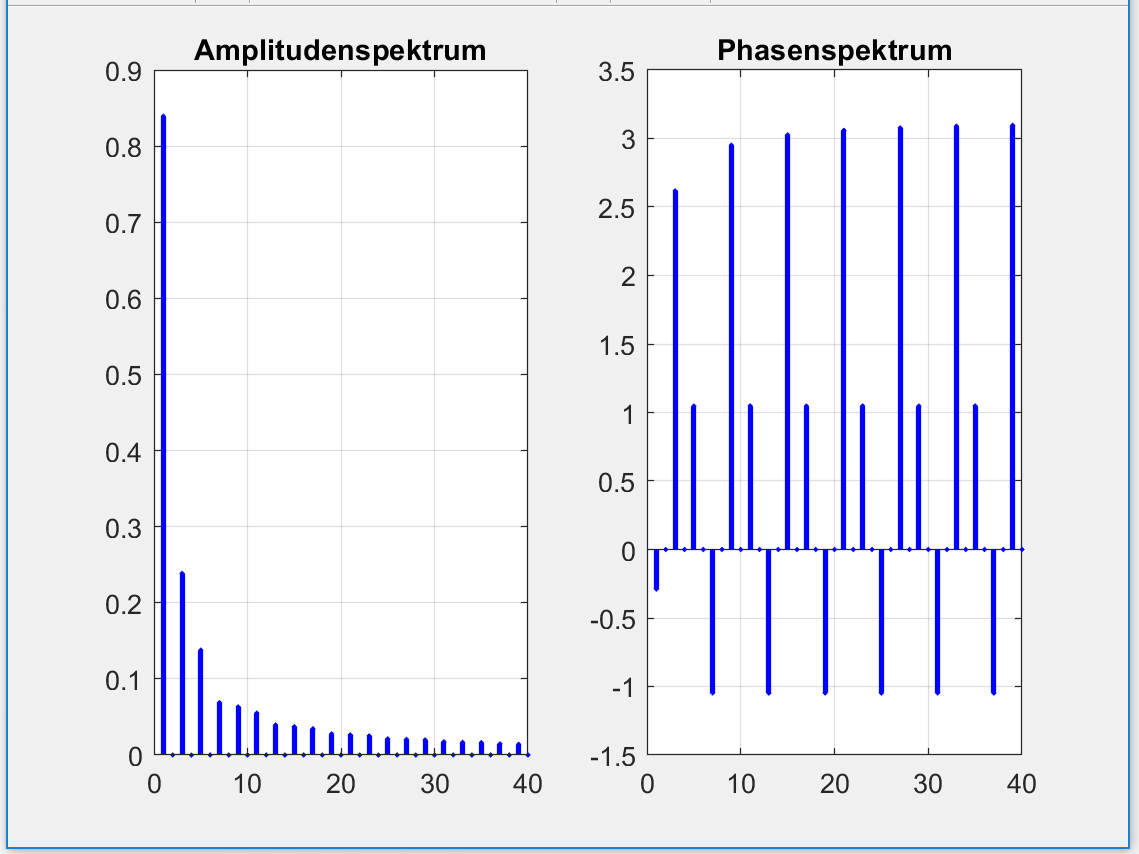
\includegraphics[width=0.47\linewidth]{A_PH_60.png}\label{fig:Amplituden-und_Phasenspektrum_60}}\qquad
	\subfloat[][]{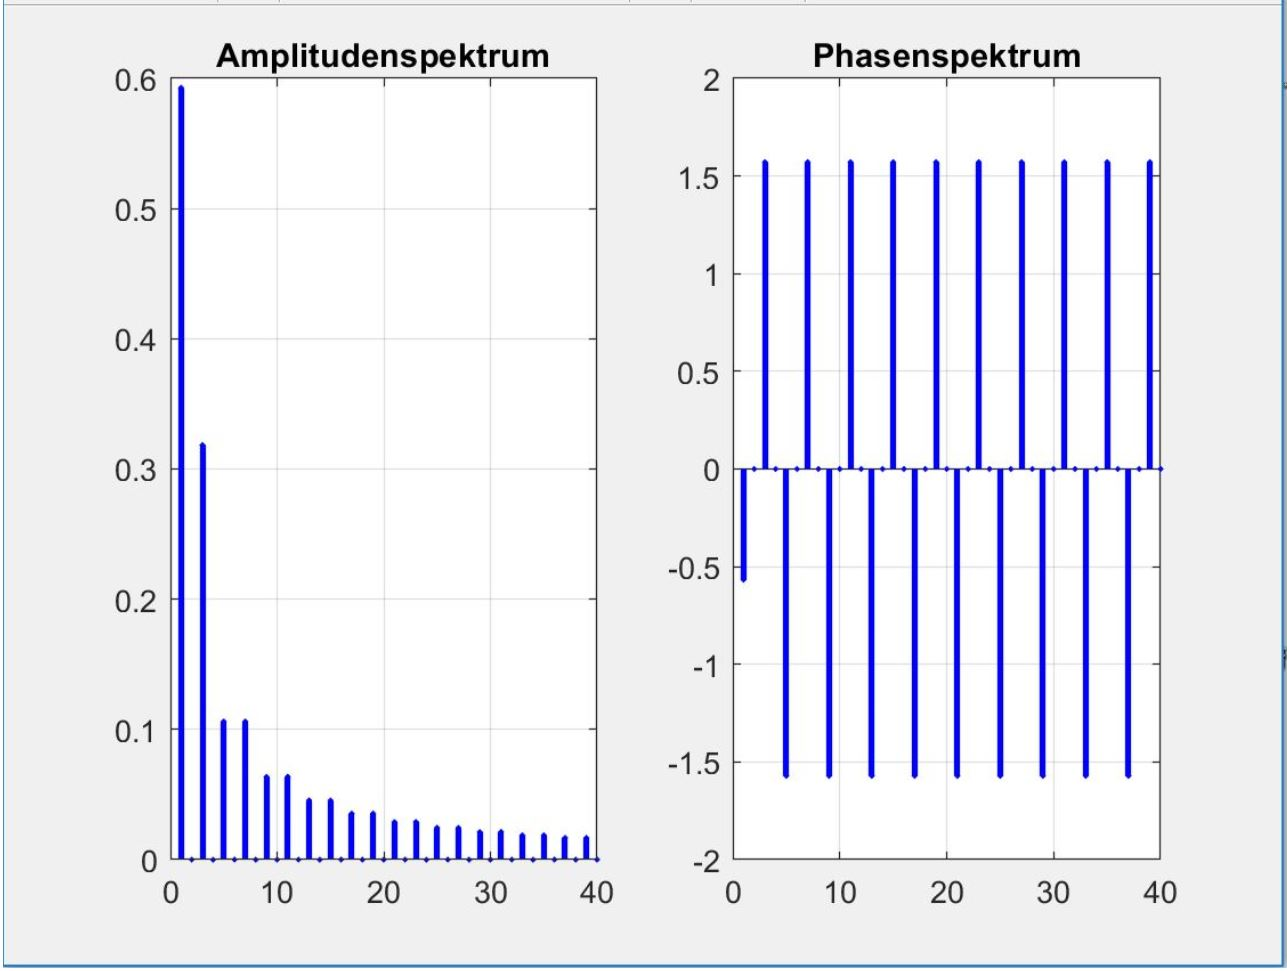
\includegraphics[width=0.47\linewidth]{A_PH_90.png}\label{fig:Amplituden-und_Phasenspektrum_90}}
	\caption{Amplituden- und Phasenspektrum (a) 60\textdegree \hspace{0.02cm} (b) 90\textdegree}
	\label{fig:Amplituden- und Phasenspektrum}
\end{figure} 

Zur Kontrolle der Berechnungen des Amplituden- und Phasenspektrums wird mit den zwei Spektren das Eingangssignal rekonstruiert. Die Signale sind in Abbildung \ref{fig:Rekonstruiertes Signal} erkennbar. Es ist ersichtlich, dass die Rundung des Sinus nicht genau dem des eigentlichen Signals entspricht \ref{fig:eingangssignal_mit_Matlab}. Dies kommt daher, dass man die Funktion  \grqq nur\grqq\hspace{0.02cm} in 40 Frequenzanteile unterteilt hat. Würde man eine höhere Anzahl Anteile verwenden, so kann die Ungenauigkeiten deutlich verkleinert werden. Da man jedoch nur einen ungefähren Vergleich der beiden Funktionen haben möchte, reichen 40 Teile völlig aus.

\begin{figure}[h]
	\centering
	\subfloat[][]{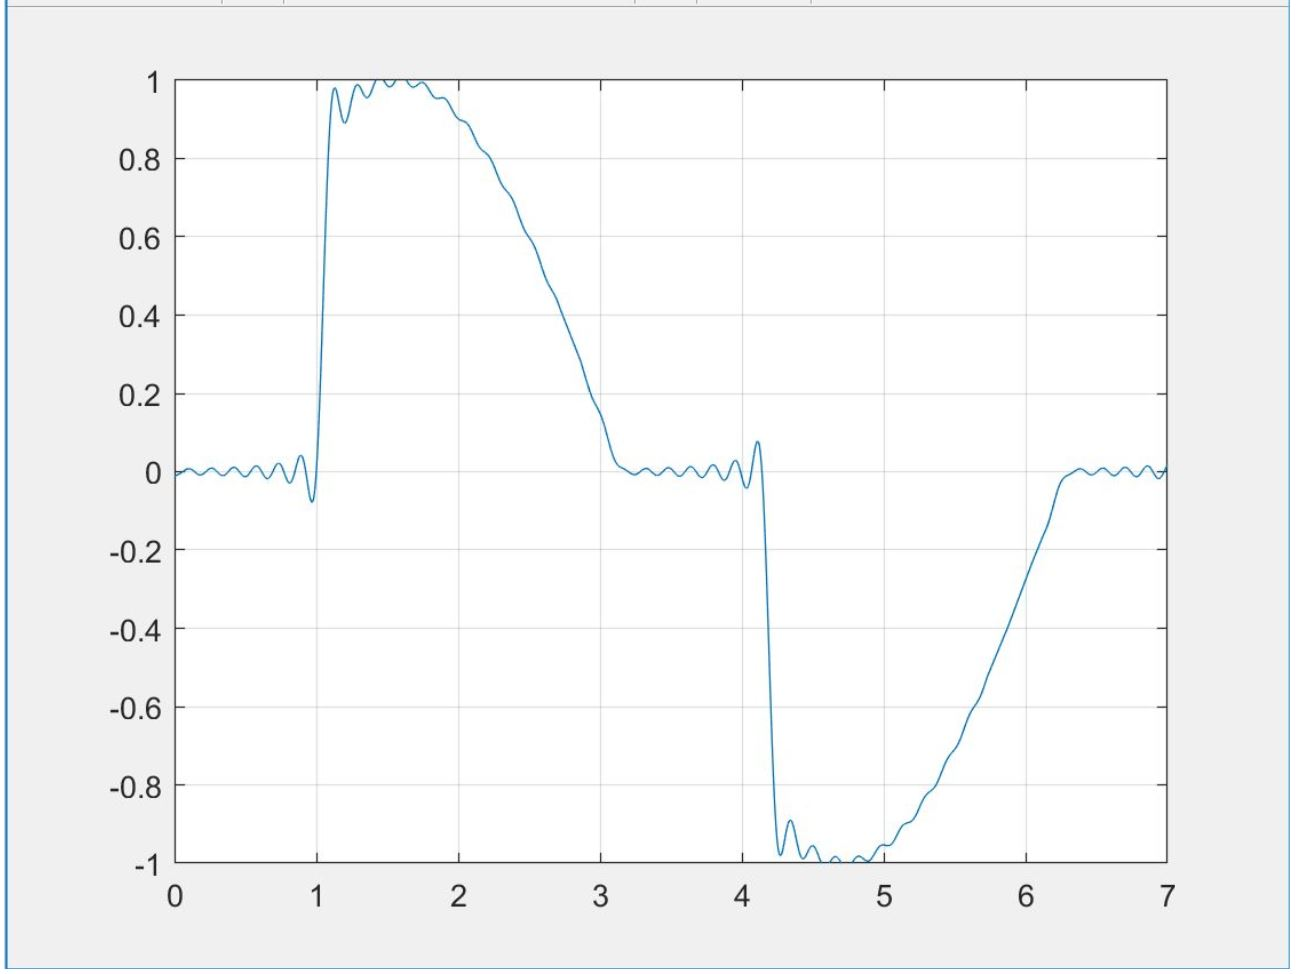
\includegraphics[width=0.47\linewidth]{re_eingangssignal_60.png}\label{fig:rekonstruiertes Signal 60}}\qquad
	\subfloat[][]{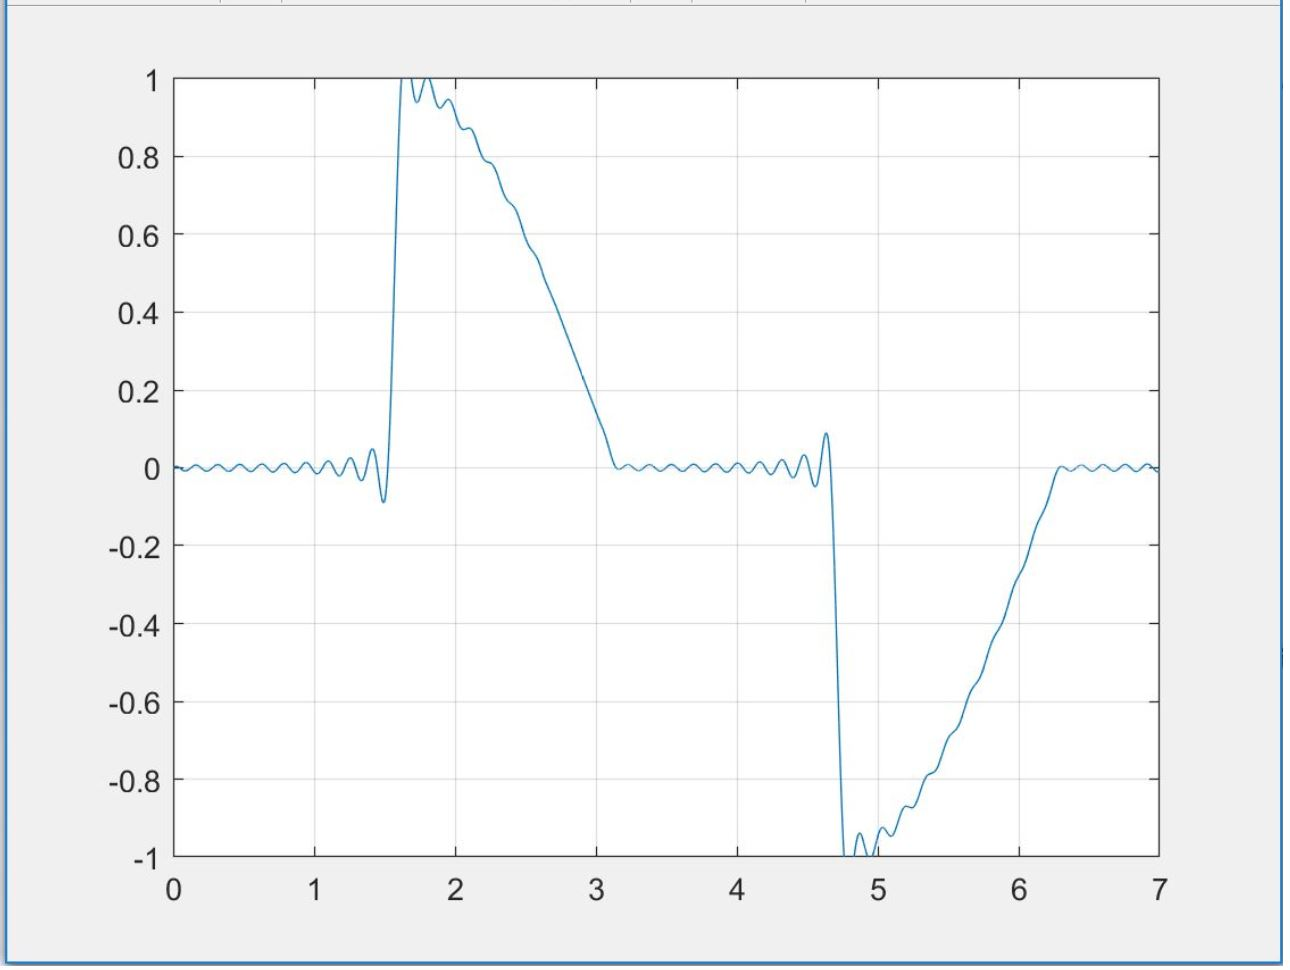
\includegraphics[width=0.47\linewidth]{re_einganssignal_90.png}\label{fig:rekonstruiertes Signal 90}}
	\caption{Rekonstruiertes Signal (a) 60\textdegree \hspace{0.02cm} (b) 90\textdegree}
	\label{fig:Rekonstruiertes Signal}
\end{figure} 

\newpage
Nachdem das Phasenanschnittsignal, das Amplitudenspektrum, das Phasenspektrum und das rekonstruierte Eingangssignal analytisch berechnet und dargestellt wurden, kann man mithilfe der FFT-Funktion (Fast Fourier Transform) von Matlab die Werte aus den Grafiken überprüfen. Die folgenden Abbildungen \ref{fig:FFT_mit_Matlab} beinhalten die Plots mit den beiden Winkeln von 60\textdegree \hspace{0.02cm} in der Abbildung \ref{fig:FFT_mit_Matlab_60} und 90\textdegree \hspace{0.02cm} in der Abbildung \ref{fig:FFT_mit_Matlab_90}. Beim Amplitudenspektrum ist die x-Achse so normiert, dass die Werte ein Vielfaches der Grundfrequenz von \SI{50}{Hz} sind. So ist zum Beispiel der Wert bei \SI{500}{Hz} beim FTT zu vergleichen mit dem Wert 10 bei den von Hand berechneten Spektren. Als Resultat erkennt man, dass beide Methoden die gleichen Ergebnisse herausgegeben haben. Es kann davon ausgegangen werden, dass die Überlegung der Berechnungen korrekt waren.

\begin{figure}[h]
	\centering
	\subfloat[][]{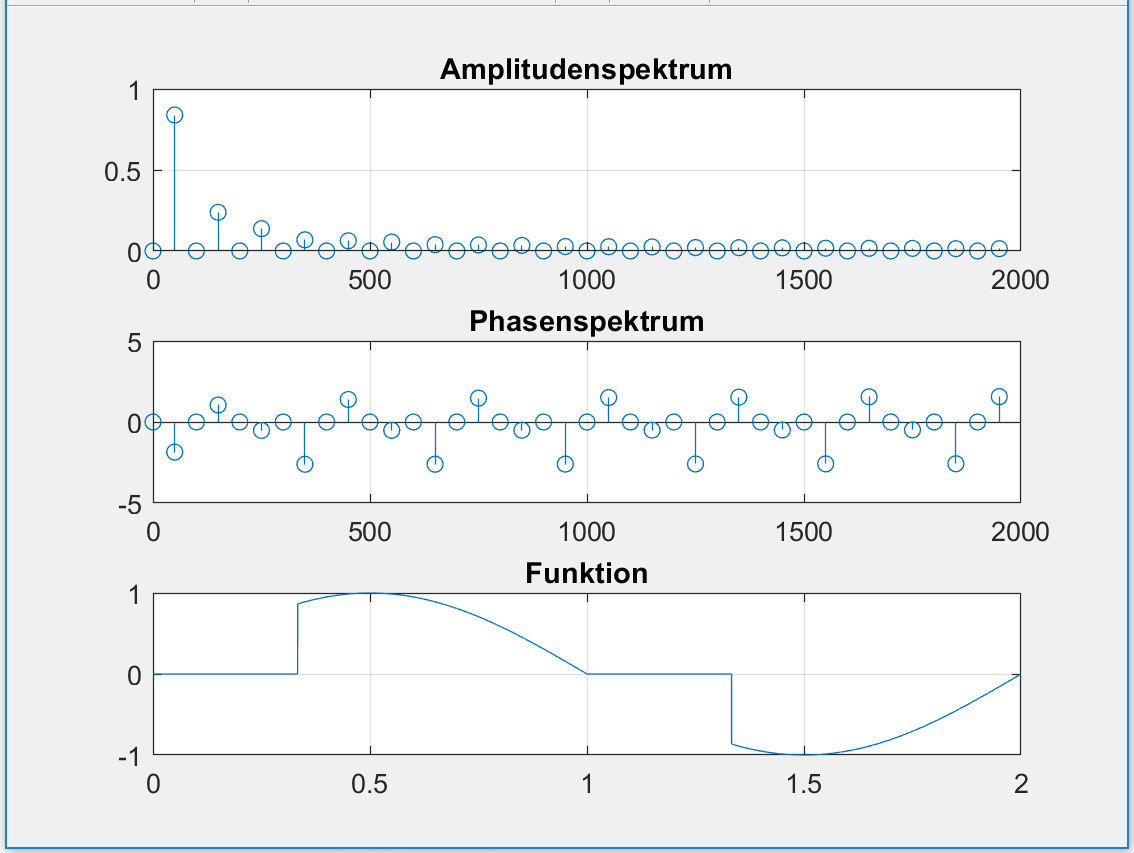
\includegraphics[width=0.47\linewidth]{FFT_mit_Matlab.png}\label{fig:FFT_mit_Matlab_60}}\qquad
	\subfloat[][]{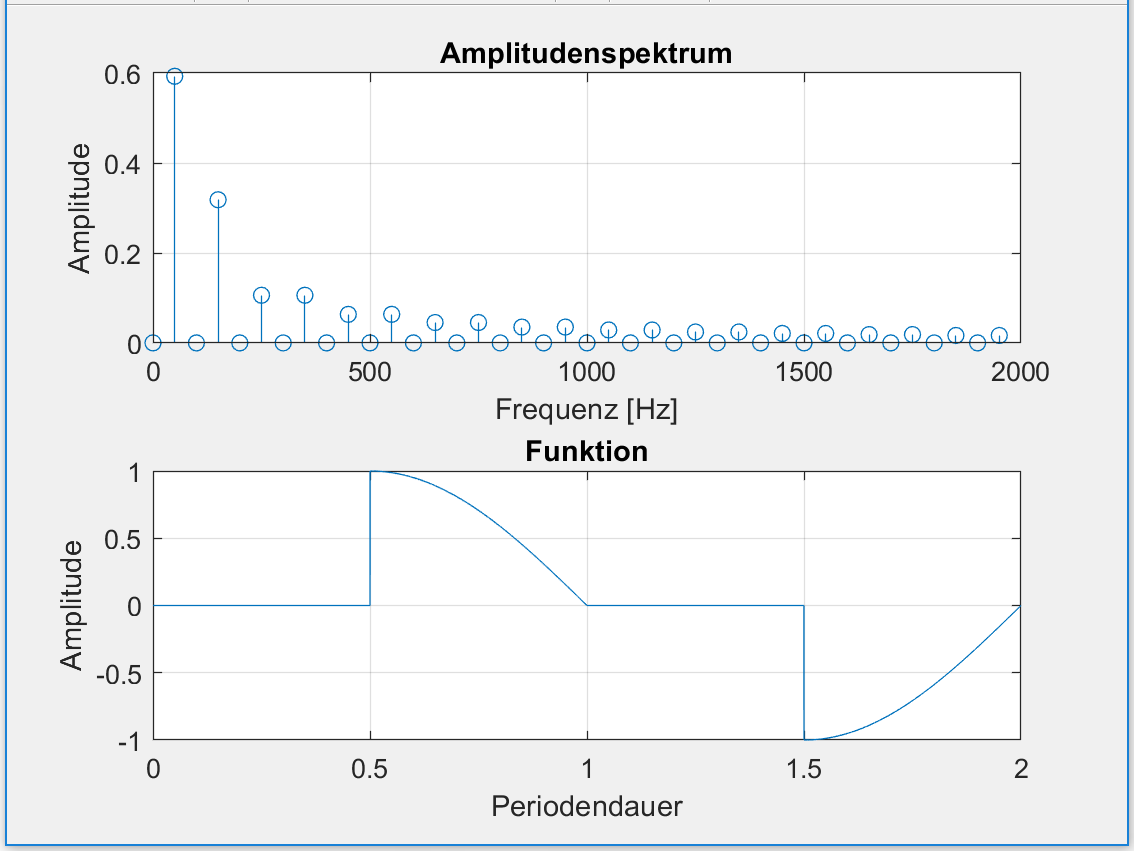
\includegraphics[width=0.47\linewidth]{FFT_mit_Matlab_90.png}\label{fig:FFT_mit_Matlab_90}}
	\caption{FFT der Matlabfunktion mit einem Winkel von (a) 60\textdegree \hspace{0.02cm} (b) 90\textdegree}
	\label{fig:FFT_mit_Matlab}
\end{figure}

\newpage

\subsubsection{Einphasige Schwingungspaketsteuerung mit Duty Cycle von 0.5 und 0.8}

Bei der zweiten Funktion, die zu überprüfen und simulieren ist, handelt es sich um eine Schwingungspaketsteuerung. Die komplette Paketdauer beträgt bei den abgebildeten Funktionen 20 Halbwellen, ersichtlich in Abbildung \ref{fig:Schwingungspaket Matlab}. Verschiedene Einschaltverfahren mit verschiedenen Duty Cycles, wie zum Beispiel 0.2, 0.4, 0.5, 0.6 oder 0.8, werden untersucht. In Abbildung \ref{fig:Schwingungspaket Matlab} erkennt man im linken Bild \ref{fig:Schwingungspacket 0.5} einen Duty Cycle von 0.5. Demzufolge sind immer 10 Halbwellen ausgeschaltet und die anderen 10 eingeschaltet.
Auf dem rechten Bild \ref{fig:Schwingungspacket 0.8} beträgt der Wert des Duty Cycle 0.8. Es sind also zuerst 4 Halbwellen ausgeschaltet und die restlichen 16 Halbwellen werden angesteuert. Die anderen Funktionen mit den dazugehörigen Duty Cycles sind im Anhang im Kapitel \ref{sec:Vergleich_der_Resultate} ersichtlich. Bei beiden Simulationsmethoden sind 5 komplette Schwingungspakete untersucht worden. 

\begin{figure}[ht!]
	\centering
	\subfloat[][]{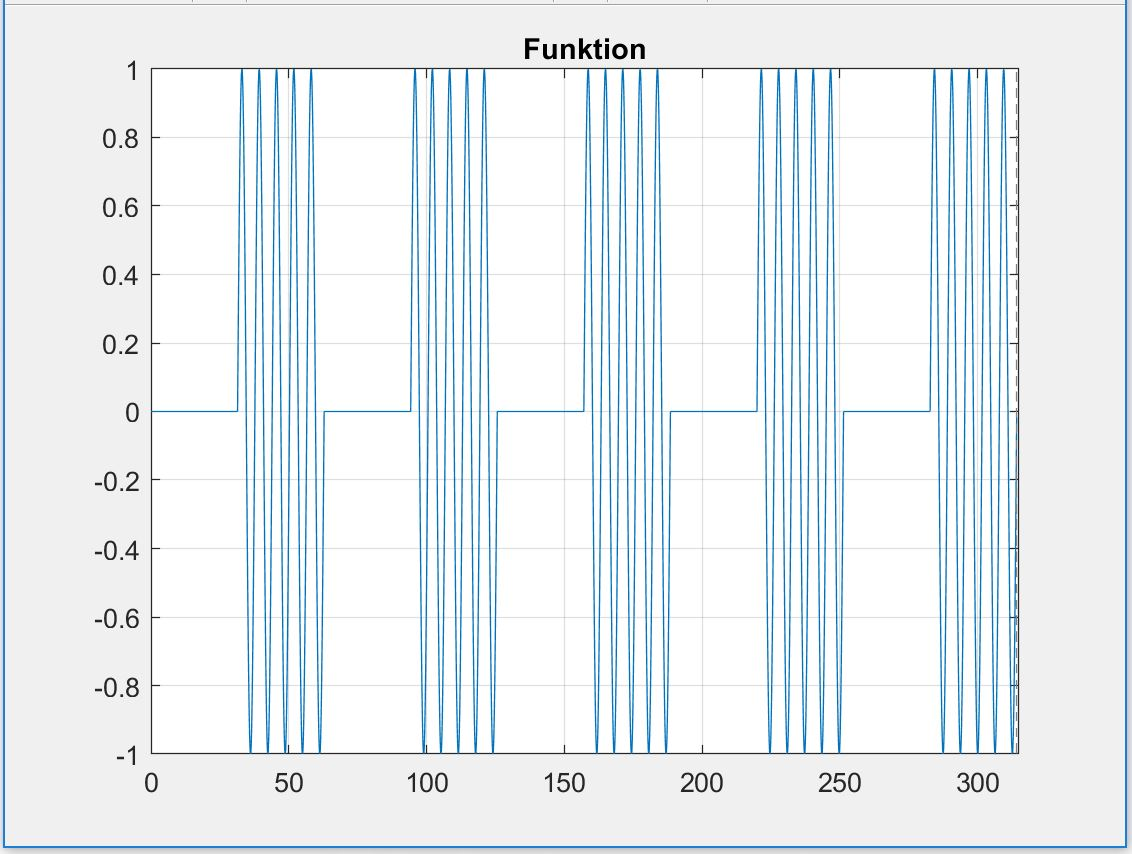
\includegraphics[width=0.43\linewidth]{Schwingungspaket_0_5.png}\label{fig:Schwingungspacket 0.5}}\qquad
	\subfloat[][]{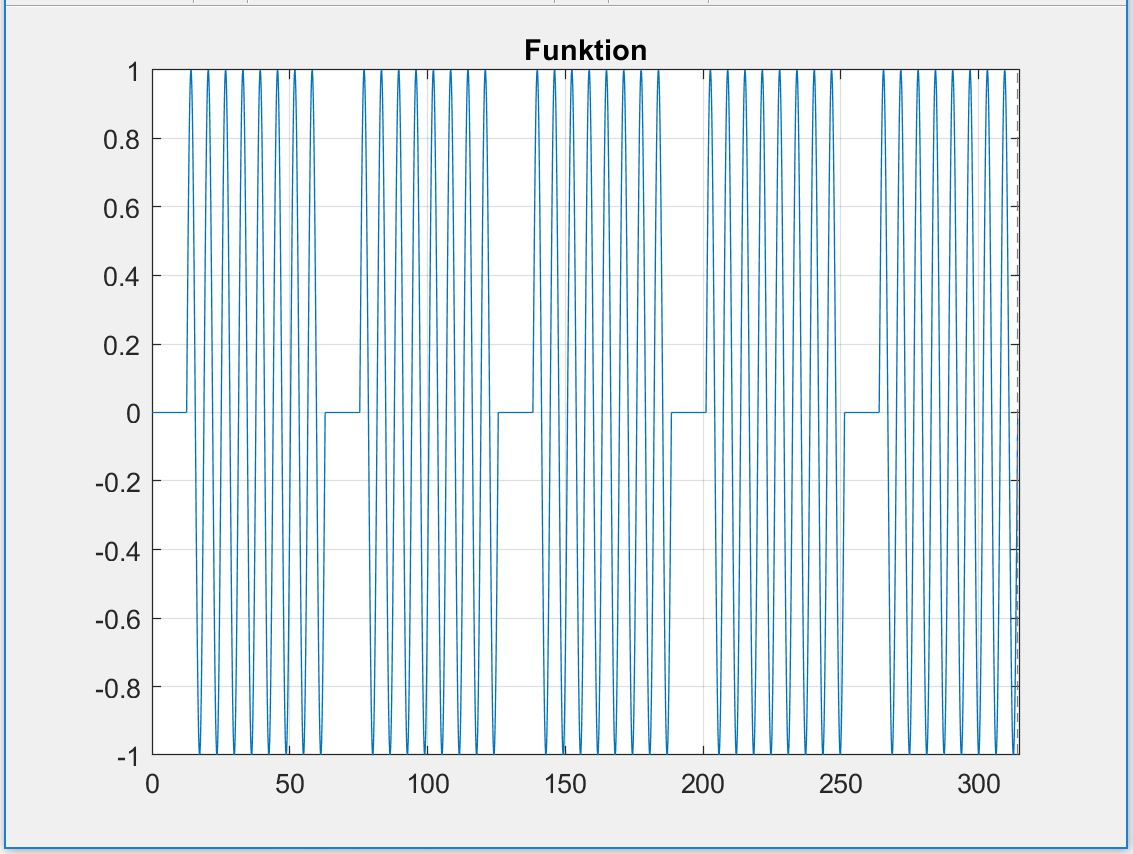
\includegraphics[width=0.43\linewidth]{Schwingungspaket_0_8.png}\label{fig:Schwingungspacket 0.8}}
	\caption{Schwingungspaket mit einem Duty Cycle von (a) 0.5 (b) 0.8}
	\label{fig:Schwingungspaket Matlab}
\end{figure} 

Um auch hier die Plecs-Simulation zu überprüfen, ist das Amplitudenspektrum absolut linear dargestellt. Bei der folgenden Abbildungen \ref{fig:Schwingungspaketspektrum Matlab} erkennt man diese Spektren. Interessant sind da vor allem die subharmonischen Schwingungen, welche sich unterhalb der Grundfrequenz von \SI{50}{Hz} befinden. Sie sind jeweils auf der linken Seite der Grafiken ersichtlich.   

\begin{figure}[ht!]
	\centering
	\subfloat[][]{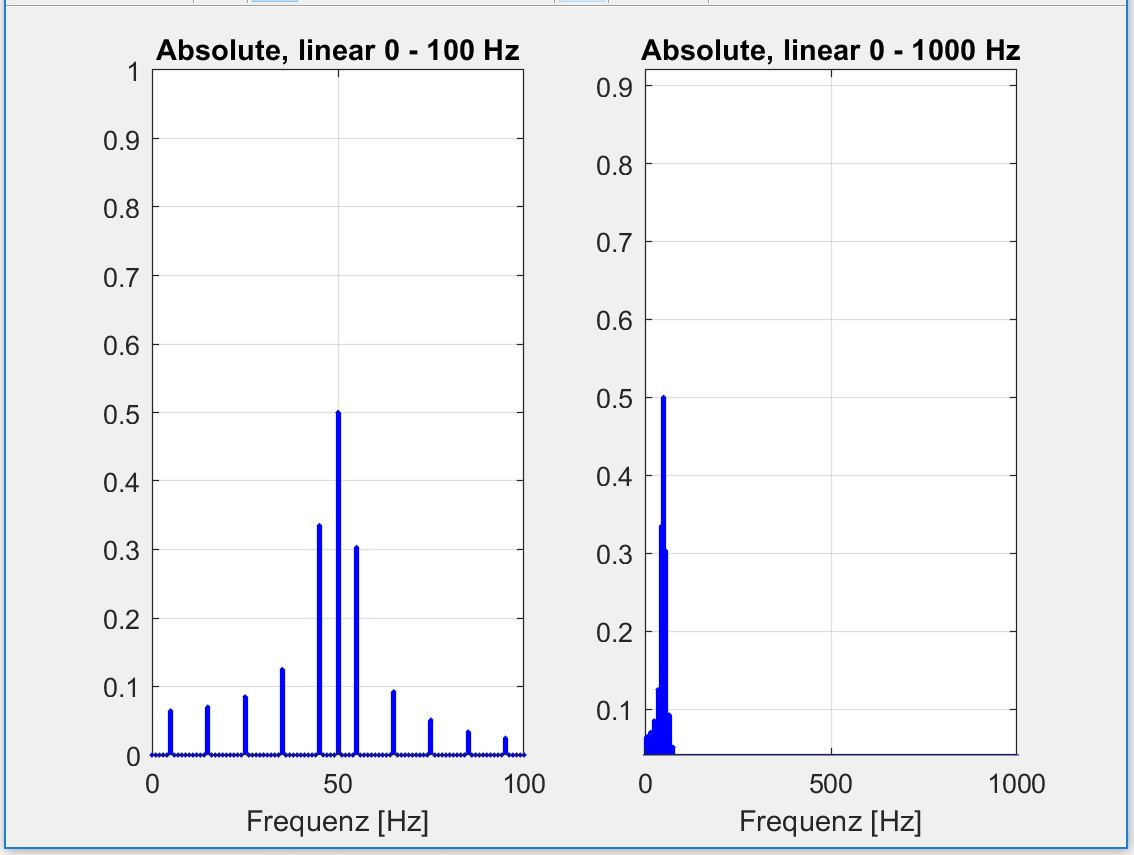
\includegraphics[width=0.47\linewidth]{Oberwellen_0_5.png}\label{fig:Schwingungspacketspektrum 0.5}}\qquad
	\subfloat[][]{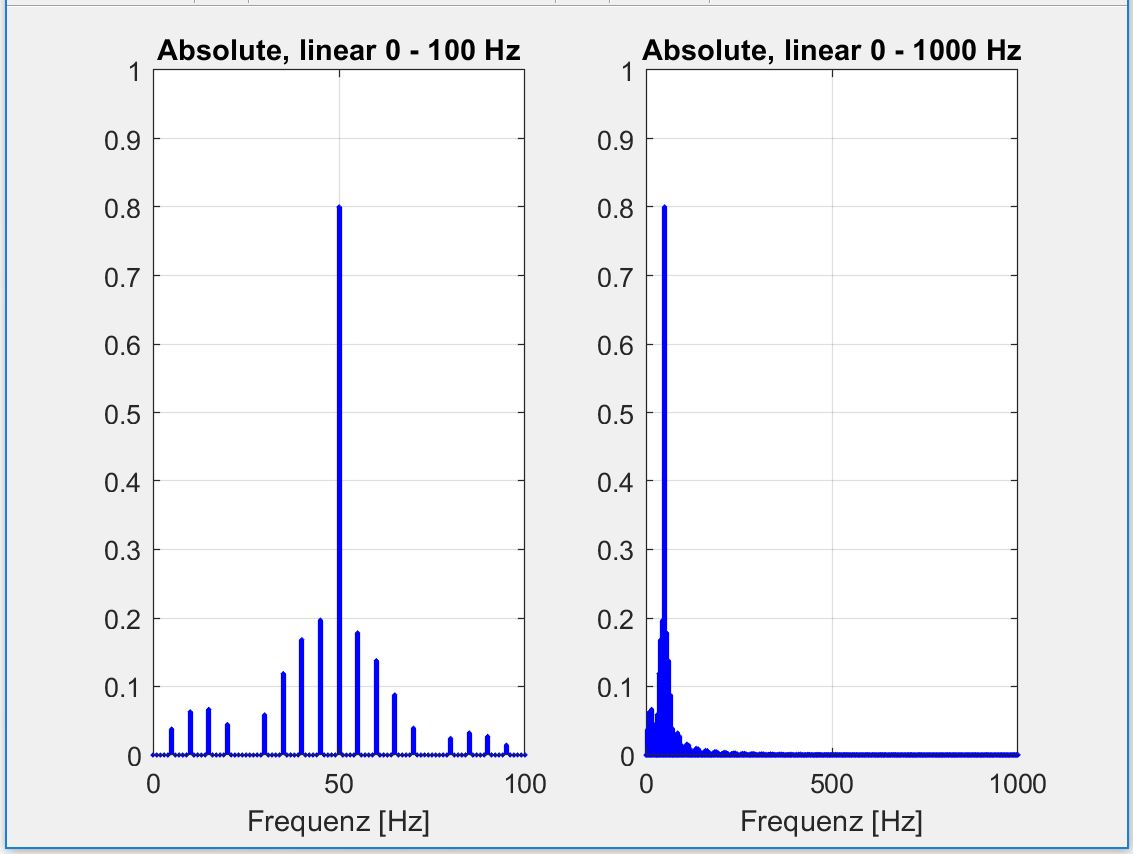
\includegraphics[width=0.47\linewidth]{Oberwellen_0_8.png}\label{fig:Schwingungspacketspektrum 0.8}}
	\caption{Lineares absolutes Spektrum mit einem Duty Cycle von (a) 0.5 (b) 0.8}
	\label{fig:Schwingungspaketspektrum Matlab}
\end{figure}

\newpage
Damit alle relevanten Oberschwingungen zu erkennen sind, ist das Spektrum bis auf \SI{1000}{Hz} erweitert worden. Dies ist auf der rechten Seite der jeweiligen Abbildung \ref{fig:Schwingungspaketspektrum Matlab} zu sehen. In Abbildung \ref{fig:Schwingungspacketspektrum 0.5} wurde das Amplitudenspektrum mit einem Duty Cycle von 0.5 dargestellt und in \ref{fig:Schwingungspacketspektrum 0.8} eines mit einem Duty Cycle von 0.8. Vergleicht man die zwei Diagramme, erkennt man, dass, je grösser der Duty Cycle ist, desto höher ist der Peak-Wert bei der Grundfrequenz von \SI{50}{Hz}. Dies erklärt sich daraus, dass bei einem grösseren Duty Cycle mehrere Sinusschwingungen vorkommen als bei einem niedrigen.\\


Die dritte Darstellungsfunktion ist der absolute Logarithmus, ersichtlich in Abbildung \ref{fig:absolut_logaritmic_matlab}. Für die Berechnung der Dämpfung [dB] verwendete man das Verhältnis der Bezugsspannung U\textsubscript{0} bei \SI{50}{Hz} mit der zu messenden Spannung U\textsubscript{n}. Auch hier sind die bereits bekannten Duty Cycle Werte von 0.5 in Abbildung  \ref{fig:absolut_logarithmic_0.5} und 0.8 in der Abbildung \ref{fig:absolut_logarithmic_0.8} verwendet worden, um den absoluten Logarithmus anzuzeigen. Diese Darstellungsform  wurde verwendet, damit man einen weiteren Vergleich mit den Plecs-Simulationen erhält.


\begin{figure}[ht!]
	\centering
	\subfloat[][]{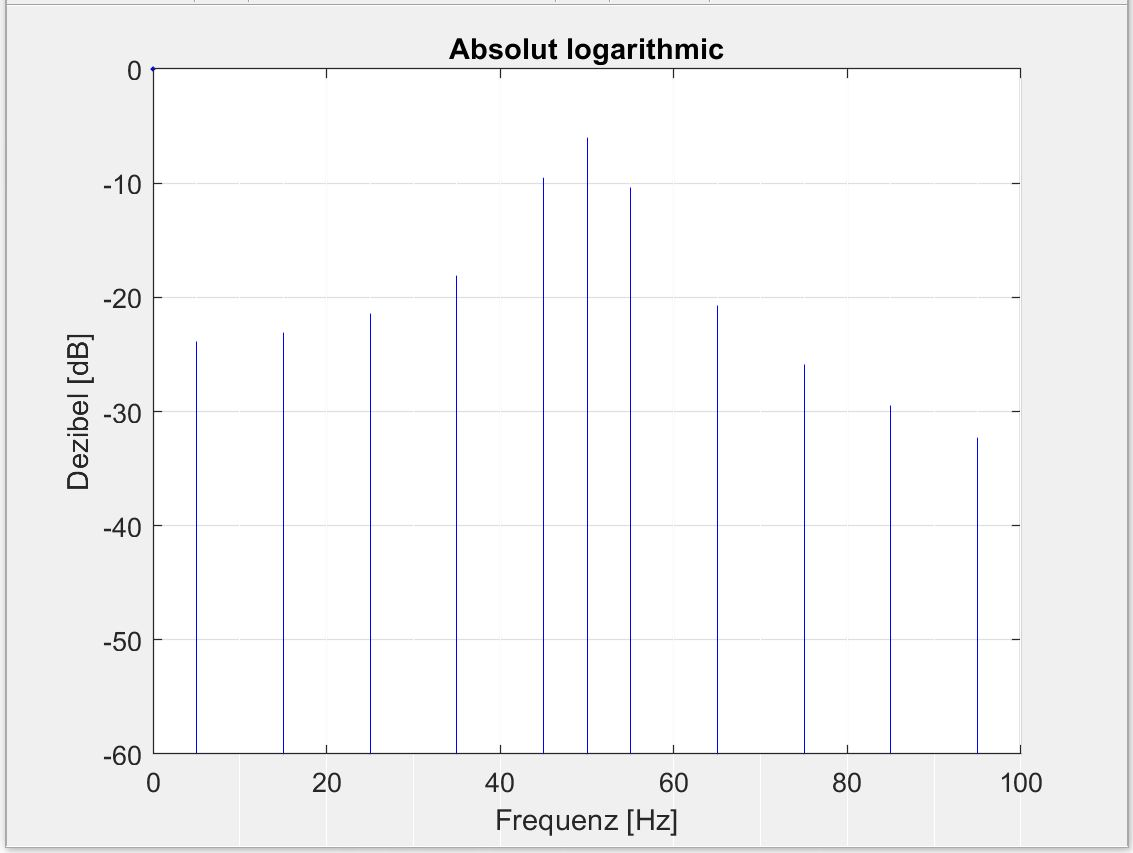
\includegraphics[width=0.45\linewidth]{absolut_logaritmic_0_5.png}\label{fig:absolut_logarithmic_0.5}}\qquad
	\subfloat[][]{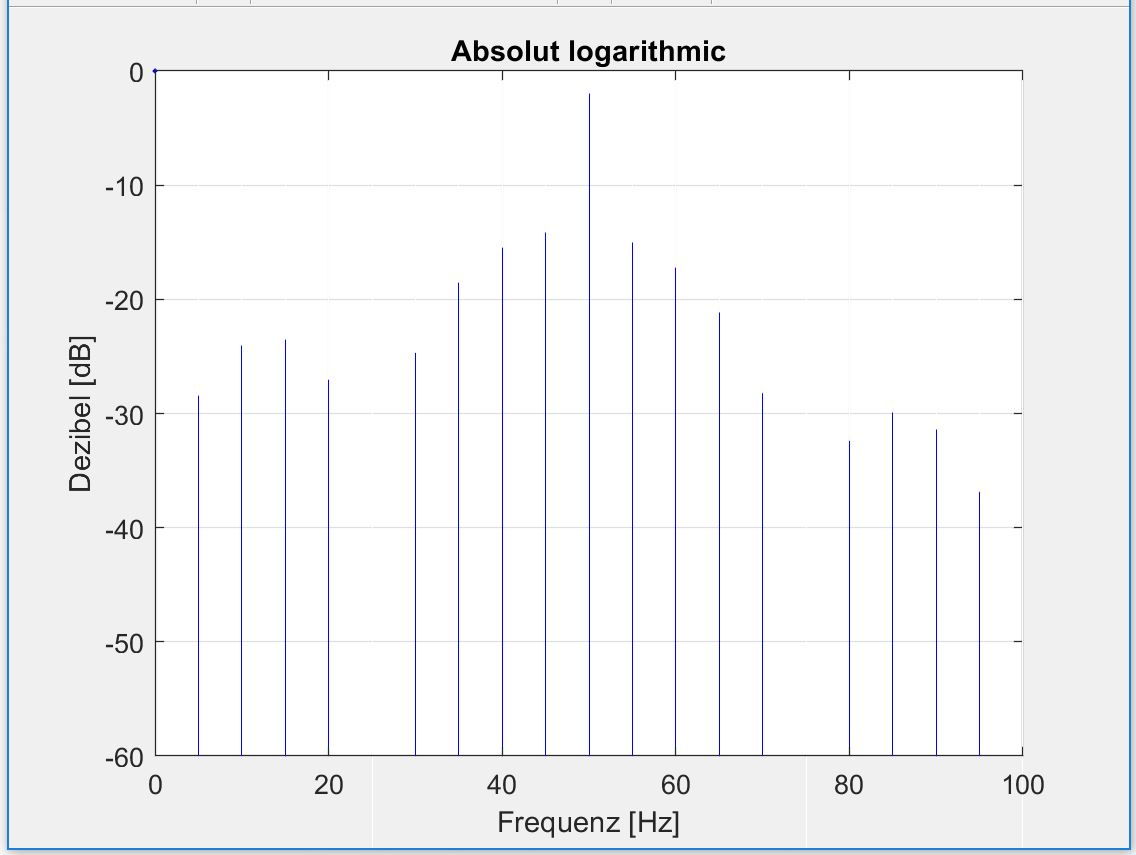
\includegraphics[width=0.45\linewidth]{absolut_logaritmic_0_8.png}\label{fig:absolut_logarithmic_0.8}}
	\caption{Lineares absolutes Spektrum mit einem Duty Cycle von (a) 0.5 (b) 0.8}
	\label{fig:absolut_logaritmic_matlab}
\end{figure}

\subsubsection{Sanftes- und hartes Hoch- und Runterfahren}\label{sec:sanftes_hoch_und_runterfahren}

In den Abbildungen \ref{fig:sanftes_Ansteuern} und \ref{fig:hartes_Ansteuern} simulierte man eine sanfte- und harte Ansteuerung der Leistung. Damit konnte das Verhalten der harmonischen- und zwischenharmonischen Oberschwingungen erkannt werden. In der Grafik \ref{fig:sanftes_Ansteuern} wählte man die Zeit des Hoch-, von \SI{200}{ms} bis \SI{1200}{ms}, und Runterfahrens, von \SI{1800}{ms} bis \SI{2800}{ms}, auf \SI{1000}{ms}. Diese Ansteuerungsart wird in diesem Beispiel als sanfte Ansteuerung bezeichnet. Die Zeit des Hoch- und Runterfahrens kann theoretisch beliebig gewählt werden. Im Bild \ref{fig:hartes_Ansteuern} wählte man die Zeit des Hoch- und Runterfahrens auf \SI{100}{ms}. Daher bestimmt man dieses Verfahren als harte Ansteuerung. 
\newpage
Visuell betrachtet ähnelt das harte Hoch- und Runterfahren viel mehr einem Rechteck als das sanfte Verfahren. Daher ist beim Amplitudenspektrum eine grössere Streuung der harmonischen- und zwischenharmonischen Oberschwingungen erkennbar. Ausserdem ist ersichtlich, dass bei der sanften Ansteuerung die Grundschwingung von \SI{50}{Hz} einen deutlich höheren Peak hat als der bei der harten Ansteuerung. Je sanfter nun die Last angesteuert wird, desto weniger verteilen sich die beiden Oberschwingungsarten in der Netzrückwirkung.


\begin{figure}[ht!]
	\centering
	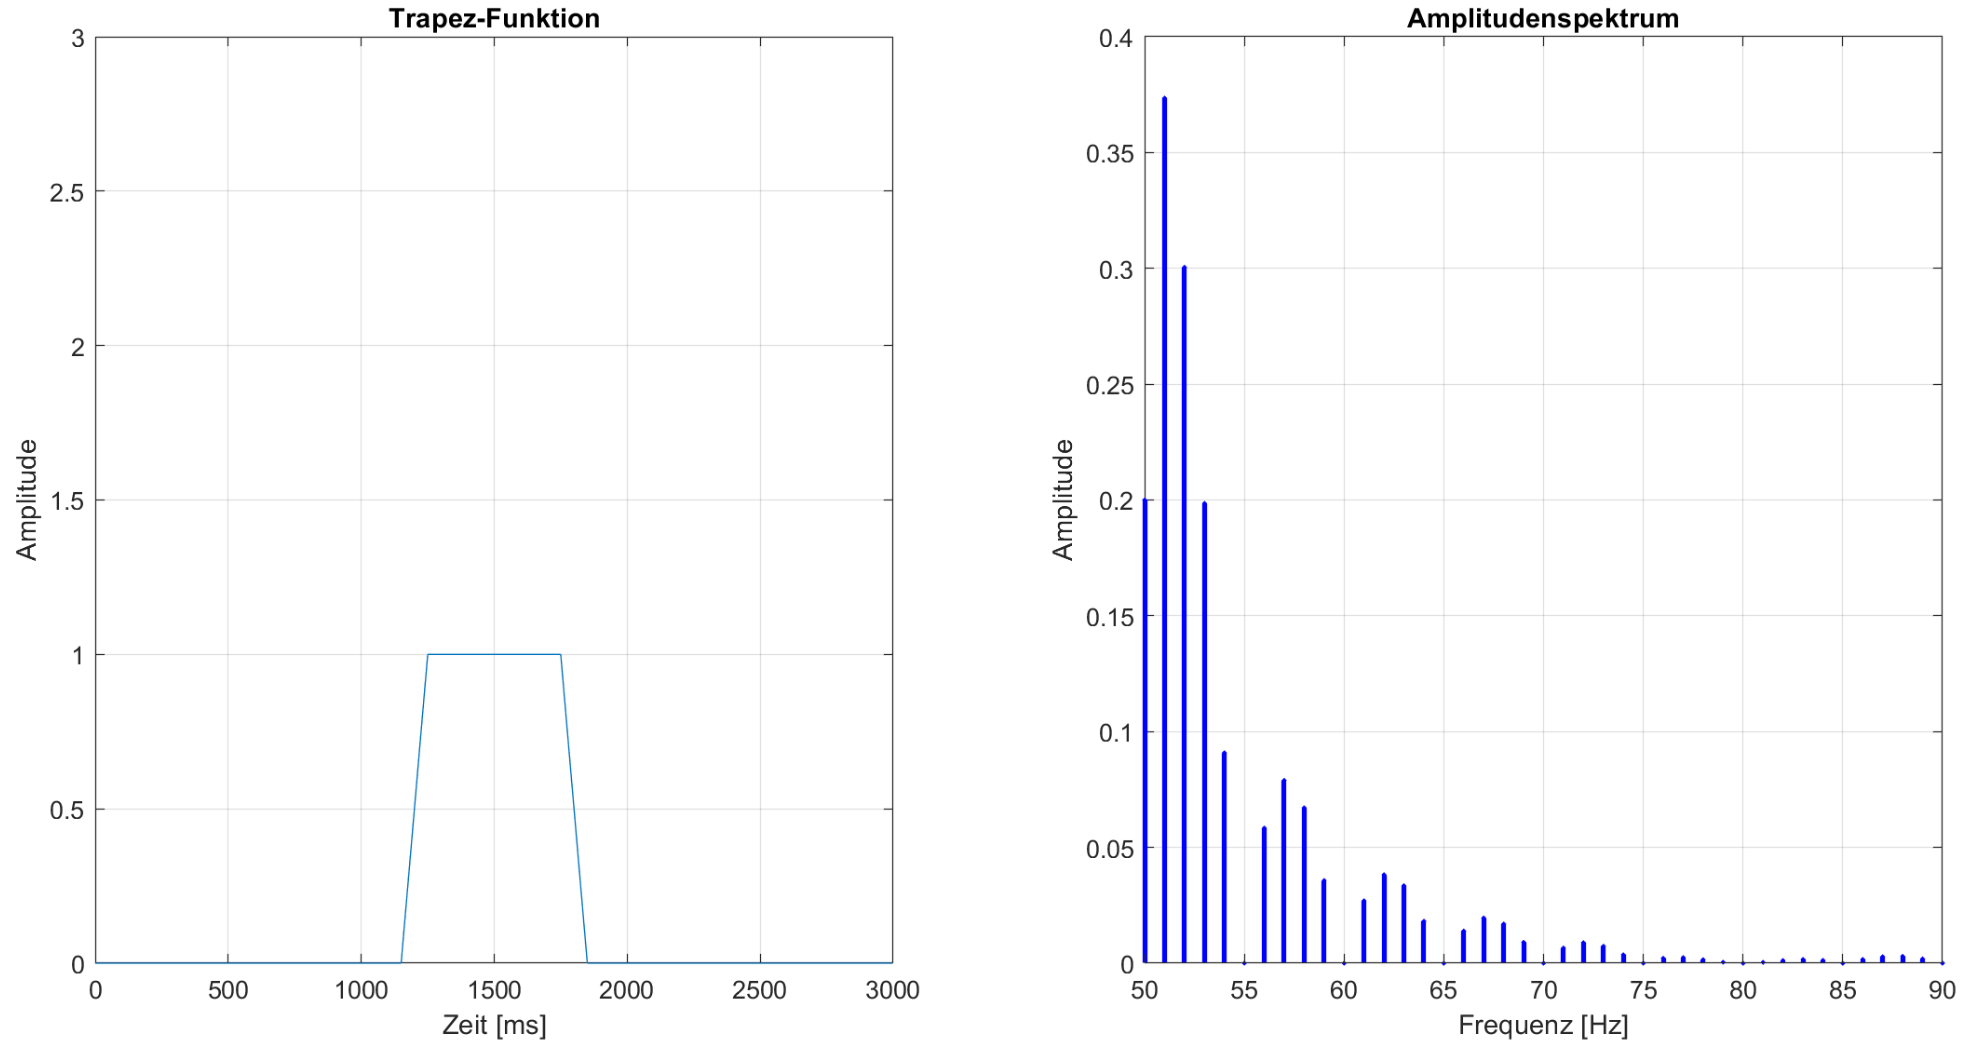
\includegraphics[scale=0.6]{sanftes_Ansteuern.png}	
	\caption{Sanftes Hoch- und Runterfahren der Leistung}
	\label{fig:sanftes_Ansteuern}
\end{figure}

\begin{figure}[ht!]
	\centering
	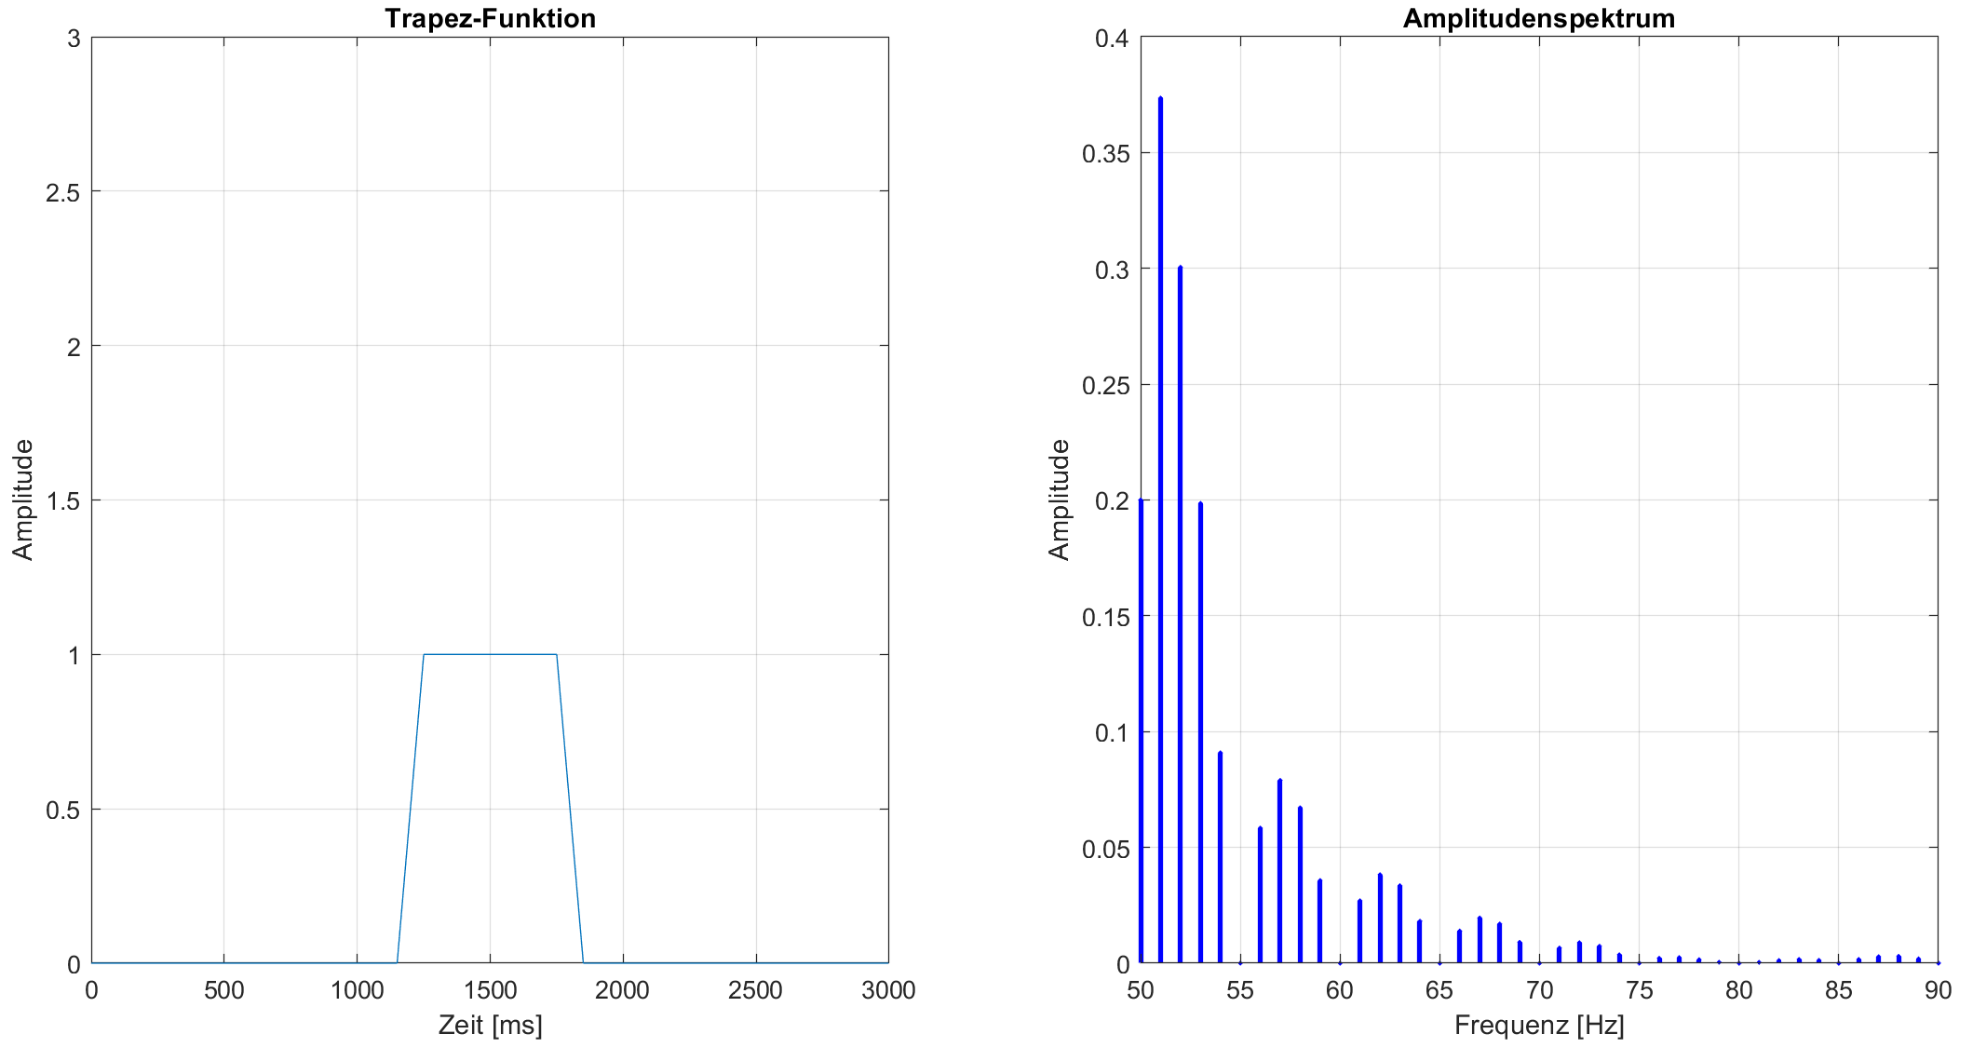
\includegraphics[scale=0.6]{hartes_Ansteuern.png}	
	\caption{Hartes Hoch- und Runterfahren der Leistung}
	\label{fig:hartes_Ansteuern}
\end{figure}




\newpage
\subsection{Simulation mit Plecs}

Mit dem Simulationsprogramm Plecs sind alle gewünschten Ansteuerungen simuliert worden. Die einphasigen Simulationen der Phasenanschnitt- und der Schwingungspaketsteuerung konnten mit den Matlab-Funktionen verglichen und ausgewertet werden. Basierend auf den verifizierten Werten ist das Verfahren für die dreiphasige Phasenanschnitt- und die Schwingungspaketsteuerung abgeleitet worden. Um von beiden Verfahren die Vorteile zu nutzen, siehe Kapitel \ref{sec:Phasenanschnittsteuerung} und \ref{sec:Schwingungspaketsteuerung}, sind die beiden Ansteuerungsarten zu einem ein- und dreiphasigen System kombiniert worden. Die Resultate sind nachfolgend erläutert.  

\subsubsection{Einphasige Phasenanschnittsteuerung mit 60\textdegree \hspace{0.02cm} und 90\textdegree}

Zuerst wird die Phasenanschnittsteuerung mit Plecs simuliert. Wie in Matlab können die verschiedenen Zündwinkel beliebig eingestellt werden. Um die Resultate vergleichen und verifizieren zu können, sind dieselben Winkel wie beim Matlab, siehe Abbildung \ref{fig:eingangssignal_mit_Matlab} gewählt. In der Abbildung \ref{fig:plecs_eingangssignal_60} erkennt man ein Sinussignal mit einem Phasenanschnitt von 60\textdegree \hspace{0.02cm}, und einen mit 90\textdegree, in der Abbildung \ref{fig:plecs_eingangssignal_90}. Die anderen Winkel mit den dazugehörigen Amplitudenspektren sind im Anhang im Kapitel \ref{sec:Vergleich_der_Resultate} ersichtlich.
Um die Spektren mit den Matlab-Simulationen vergleichen zu können, ist die Amplitude des Sinussignales auch auf \SI{1}{Volt} gestellt worden.  

\begin{figure}[ht!]
	\centering
	\subfloat[][]{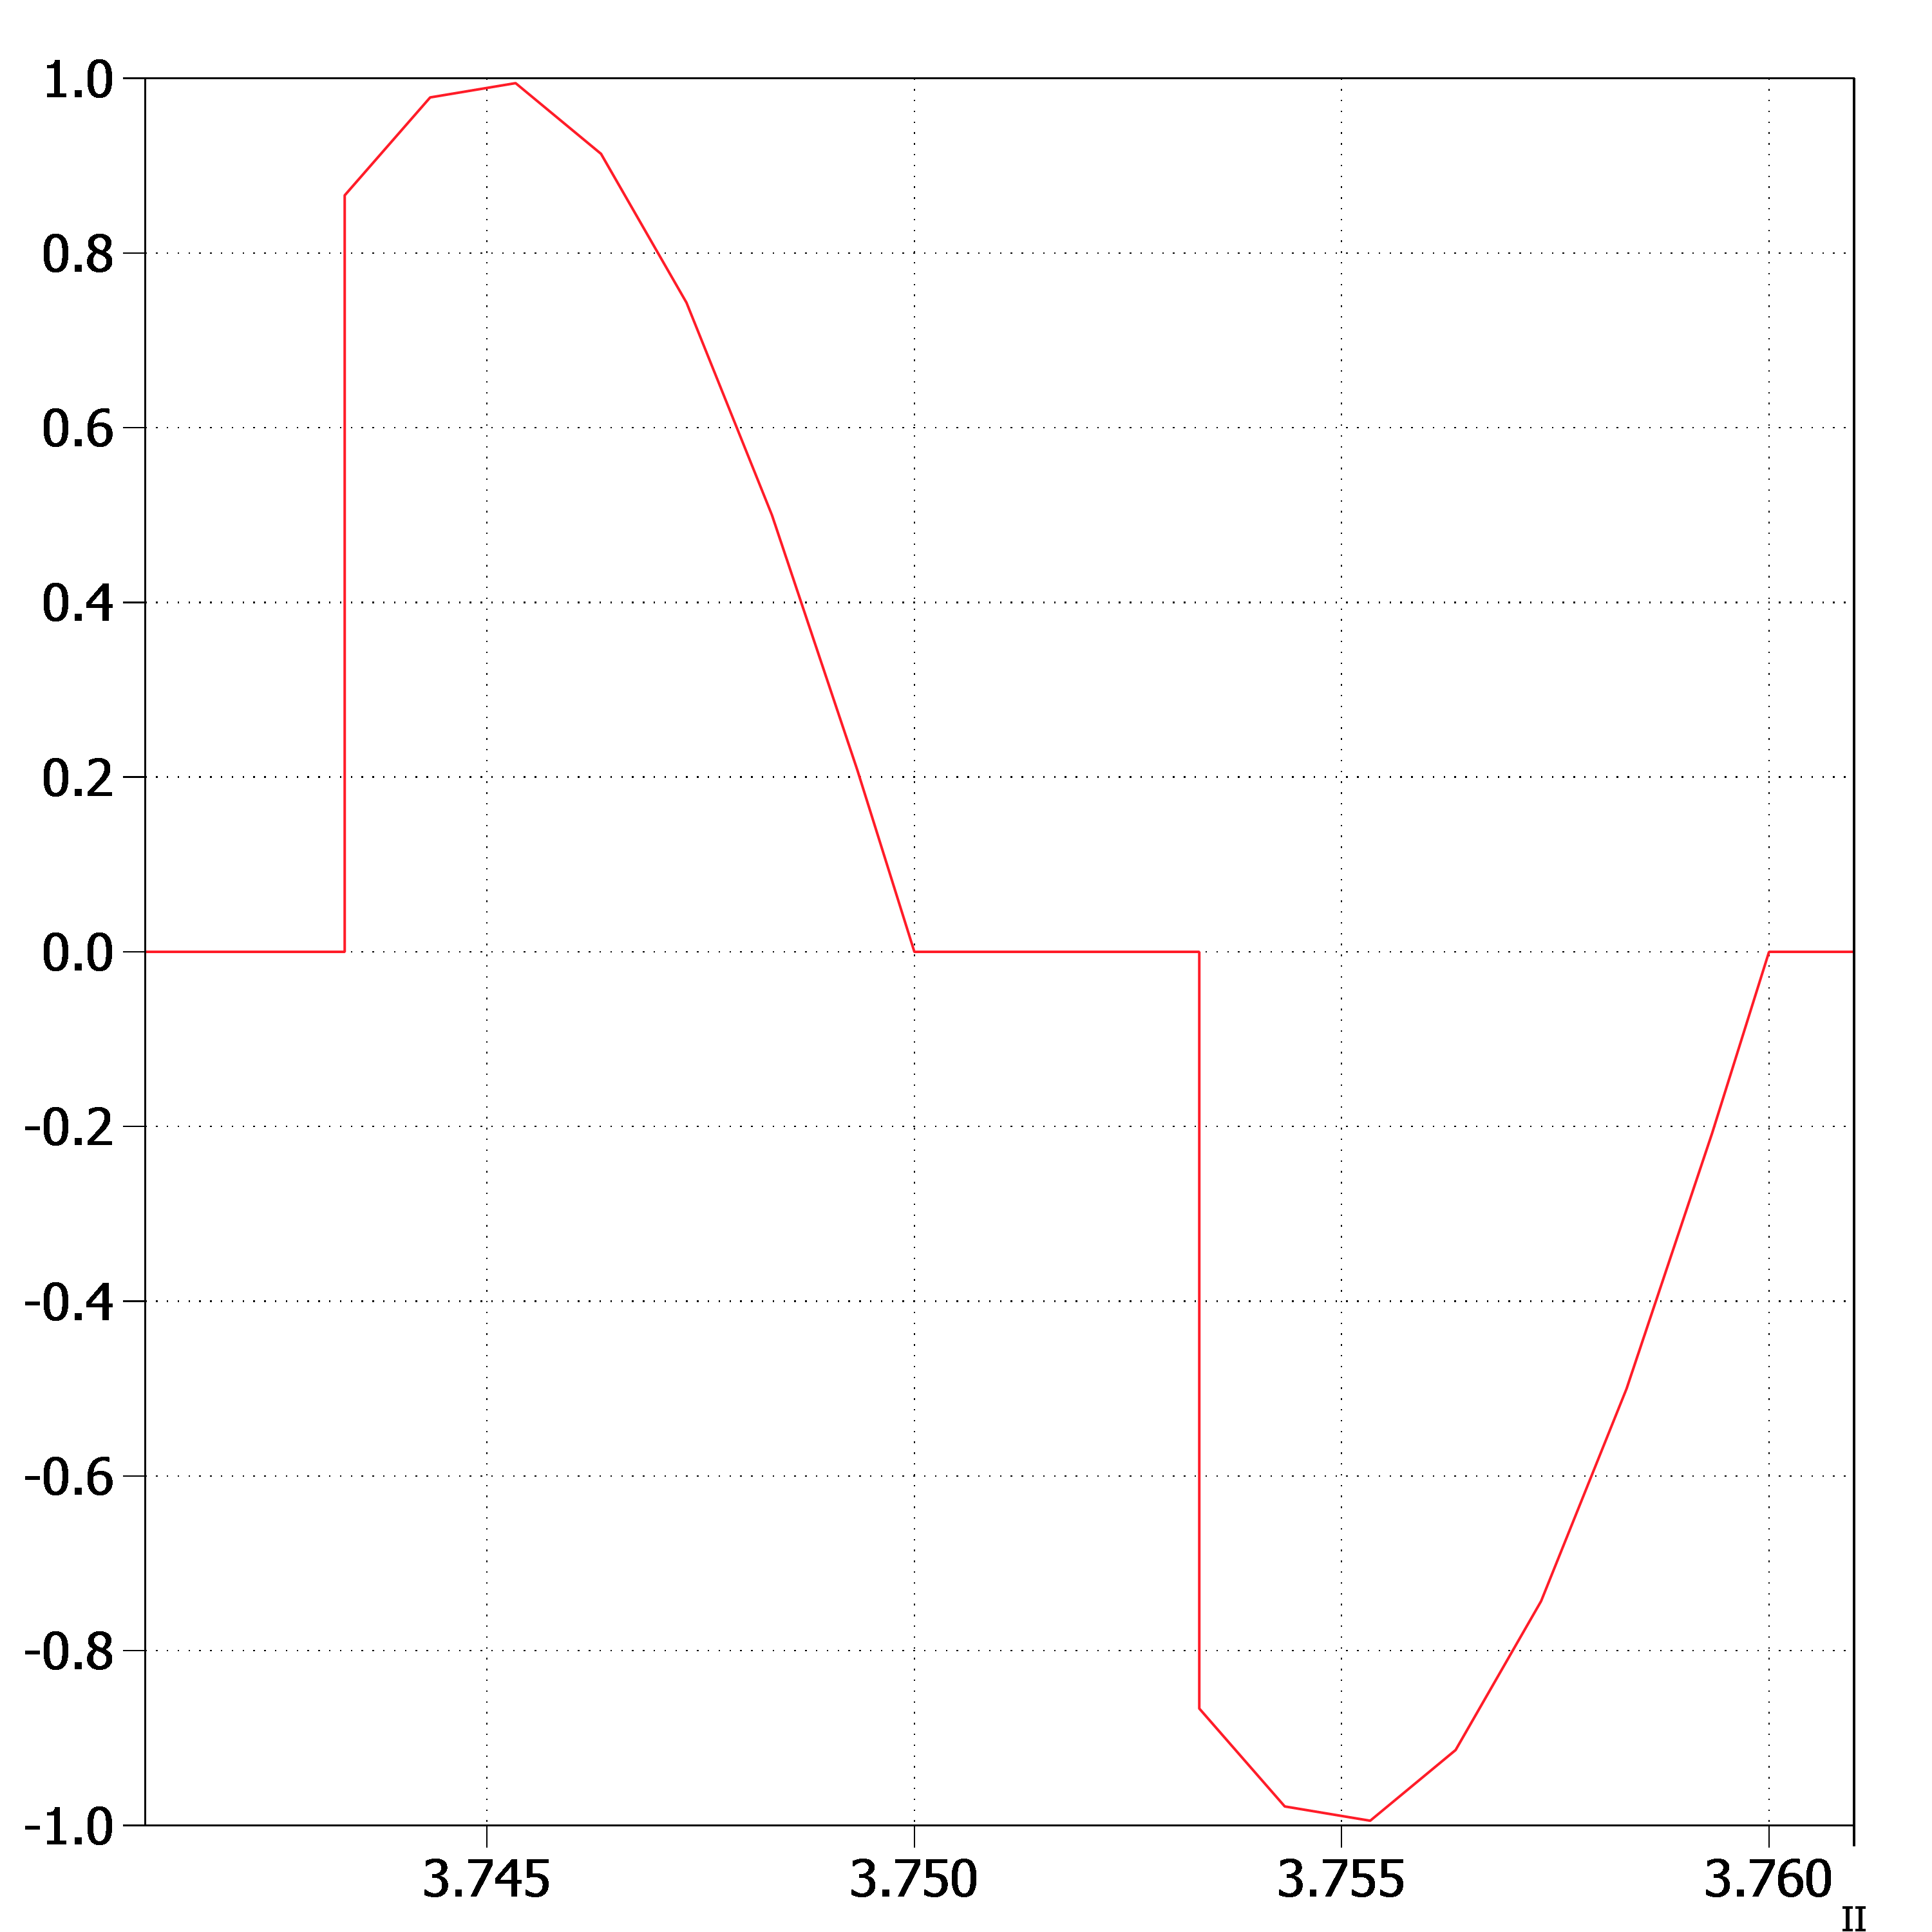
\includegraphics[width=0.43\linewidth]{plecs_phasenanschnitt_pi_3_funktion.png}\label{fig:plecs_eingangssignal_60}}\qquad
	\subfloat[][]{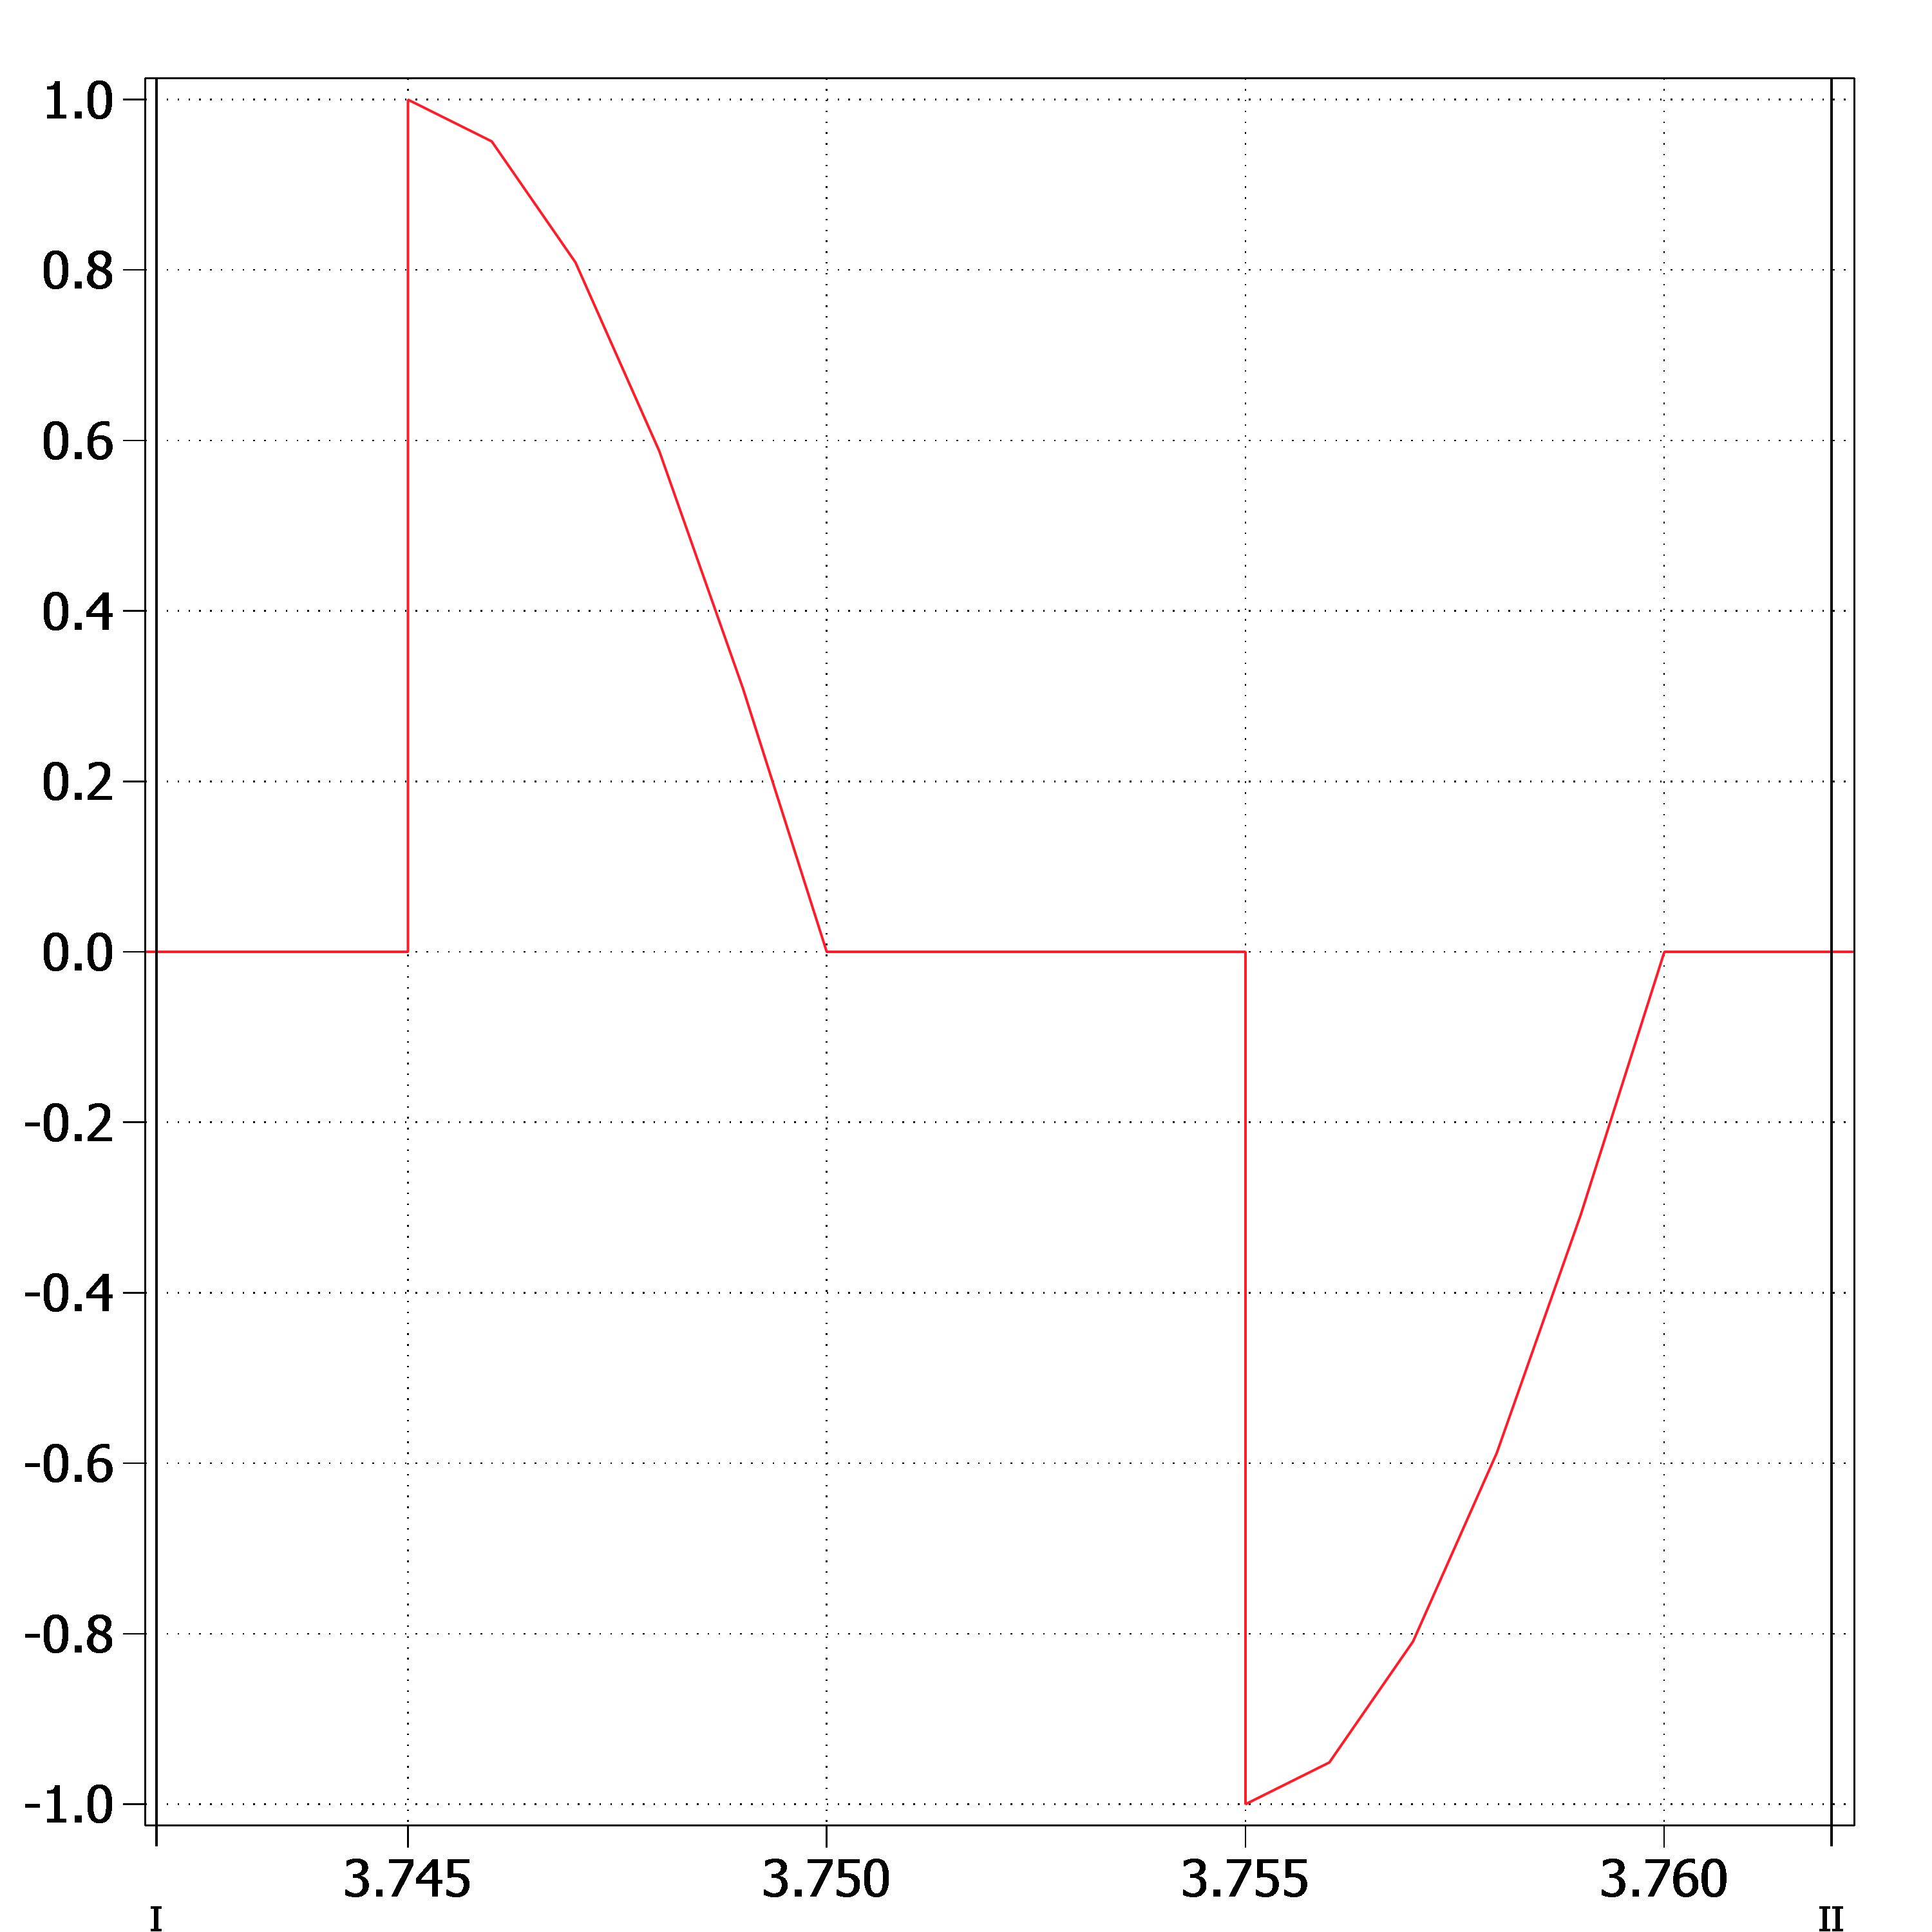
\includegraphics[width=0.43\linewidth]{plecs_phasenanschnitt_pi_2_funktion.png}\label{fig:plecs_eingangssignal_90}}
	\caption{Eingangssignal mit Phasenanschnitt (a) 60\textdegree (b) 90\textdegree}
	\label{fig:Eingangssignal simuliert mit Plecs}
\end{figure}

\newpage

Die beiden Diagramme \ref{fig:plecs_Amplitudenspektrum} zeigen das Amplitudenspektrum der Phasenanschnittsteuerung mit den zwei bereits verwendeten Winkeln. Die Grafik musste nicht wie bei der Matlab-Funktion analytisch berechnet werden, sondern konnte mithilfe des Plecs Scope direkt analysiert werden. Plecs macht auch eine Fourier-Analyse, um das Spektrum darzustellen. Vergleicht man die Amplitudenspektren der beiden Simulationen miteinander, sind die vertikalen Verläufe, nach erster Einschätzung, sehr ähnlich. Der genau Vergleich der Werte wird im Kapitel \ref{sec:Vergleich_Plecs_Matlab} analysiert.  
     
\begin{figure}[ht!]
	\centering
	\subfloat[][]{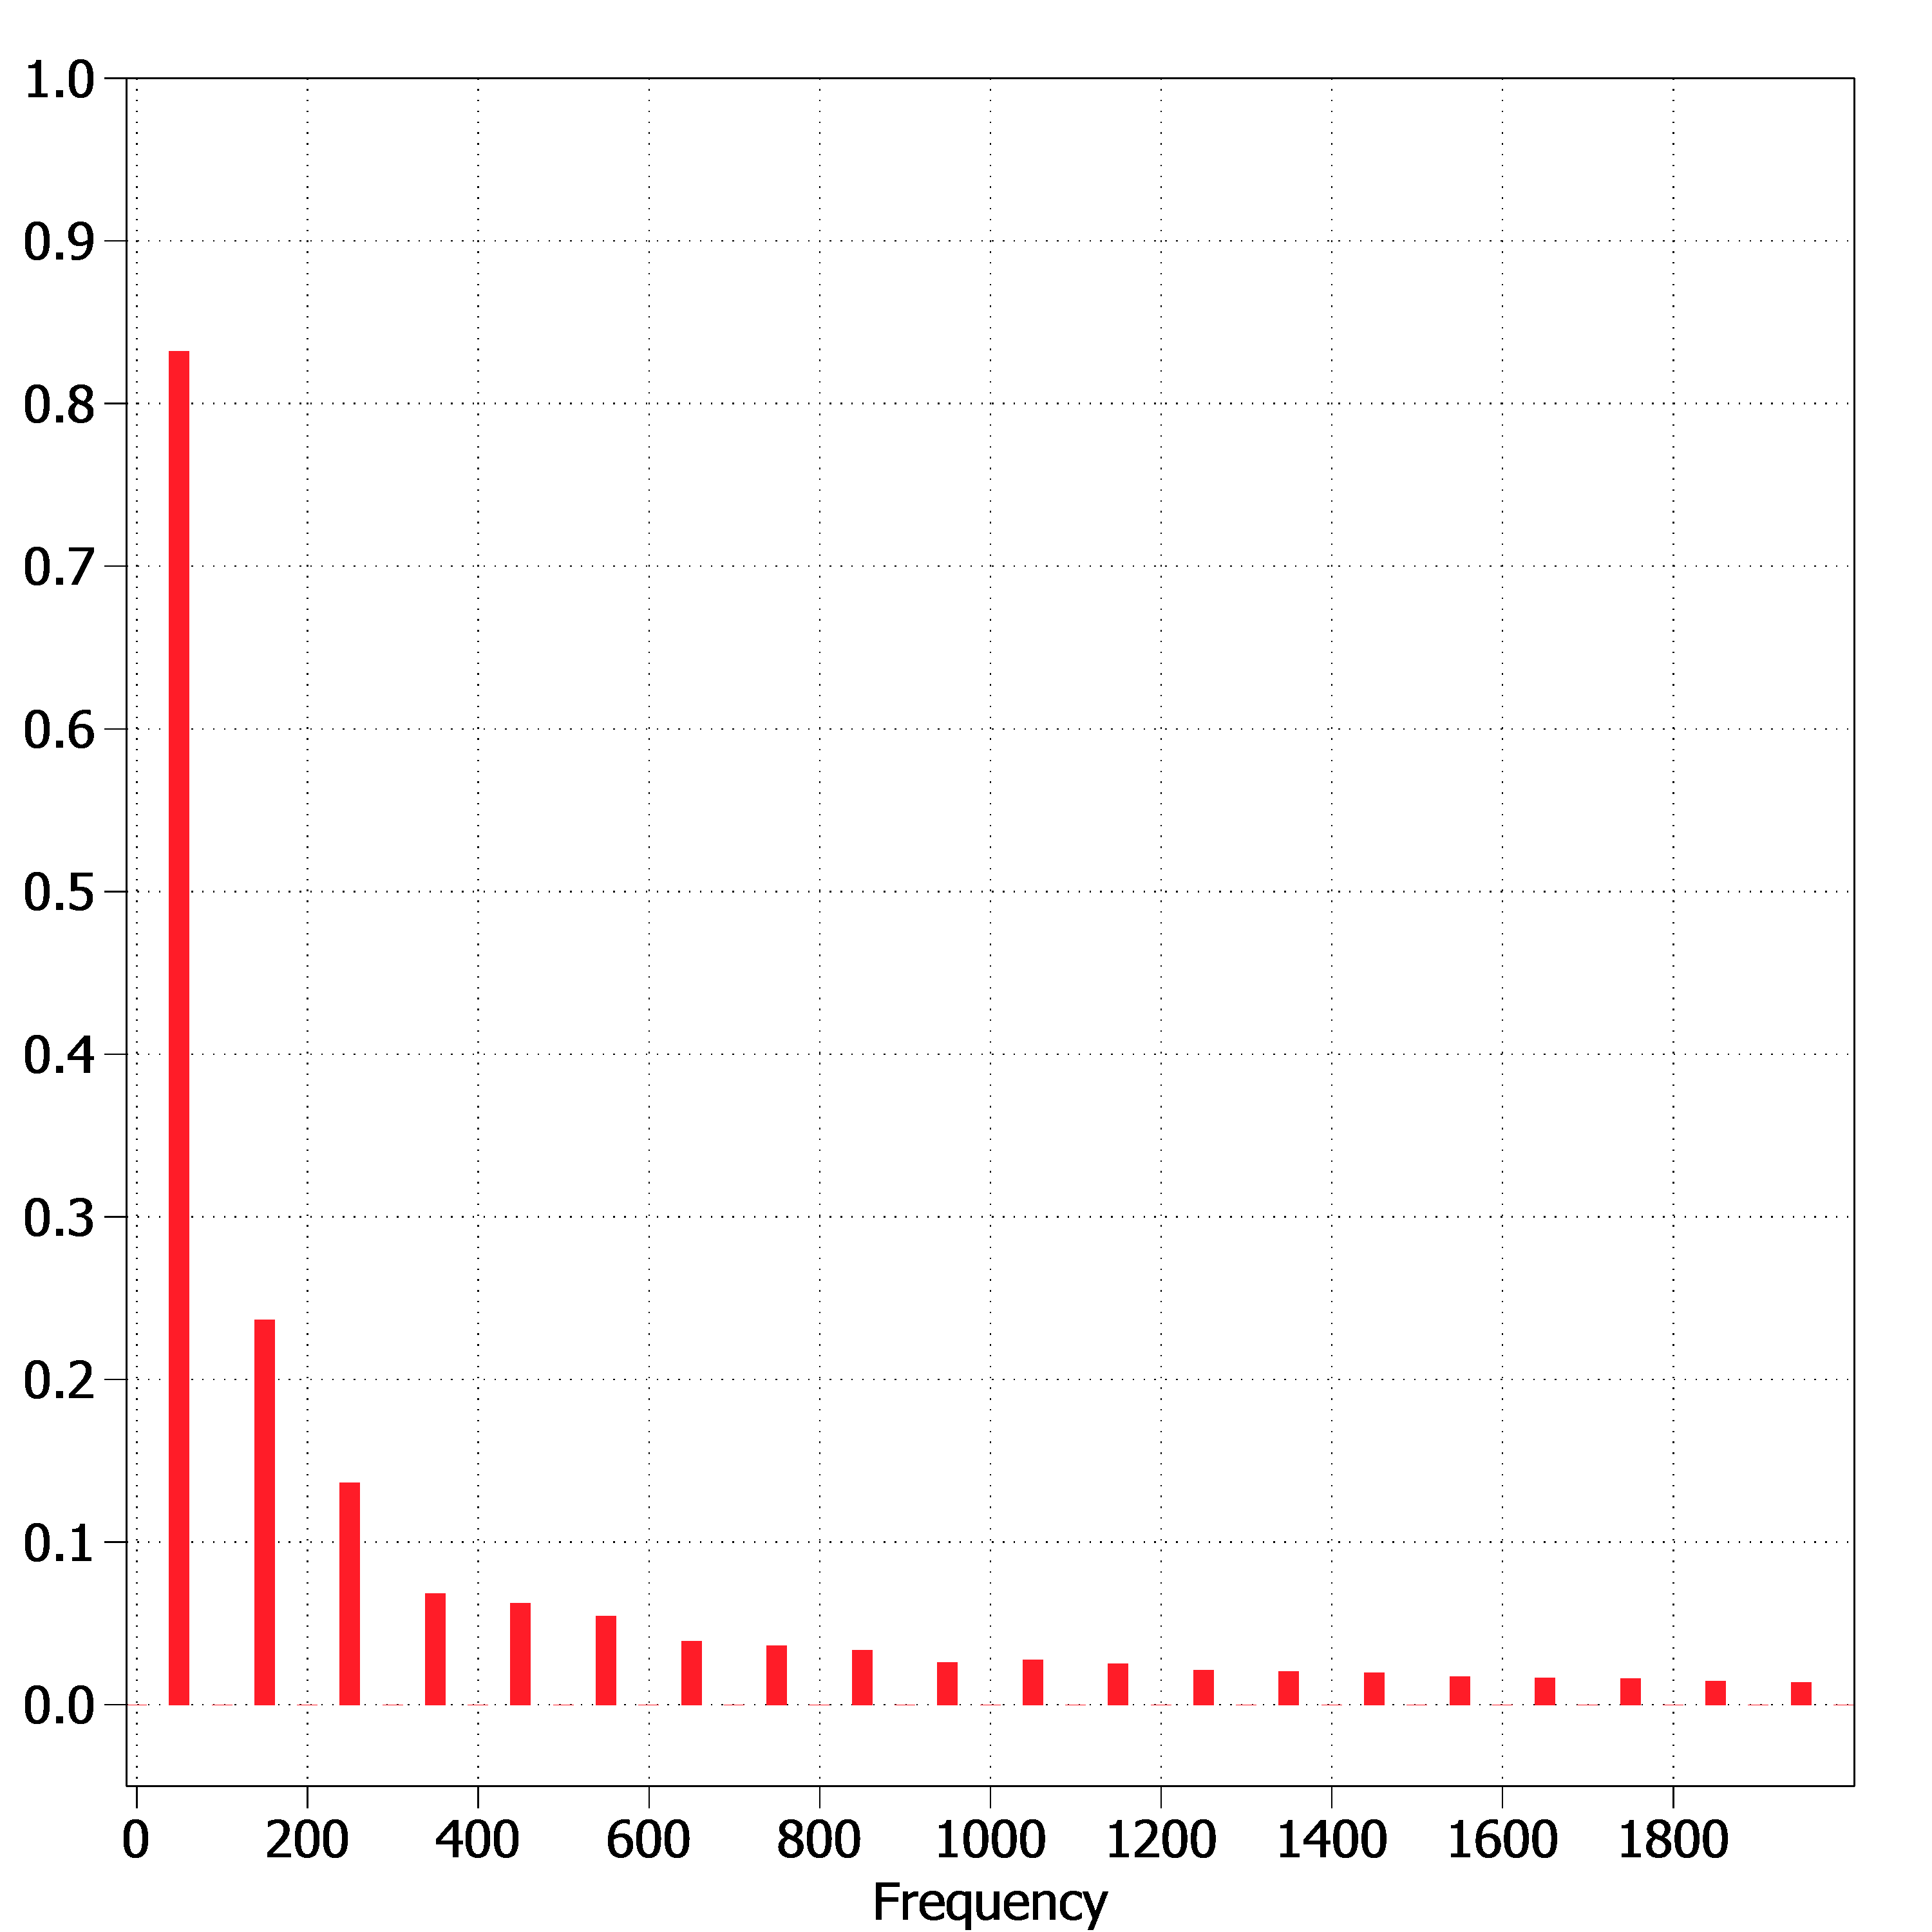
\includegraphics[width=0.43\linewidth]{plecs_phasenanschnitt_pi_3.png}\label{fig:plecs_Amplitudenspektrum_60}}\qquad
	\subfloat[][]{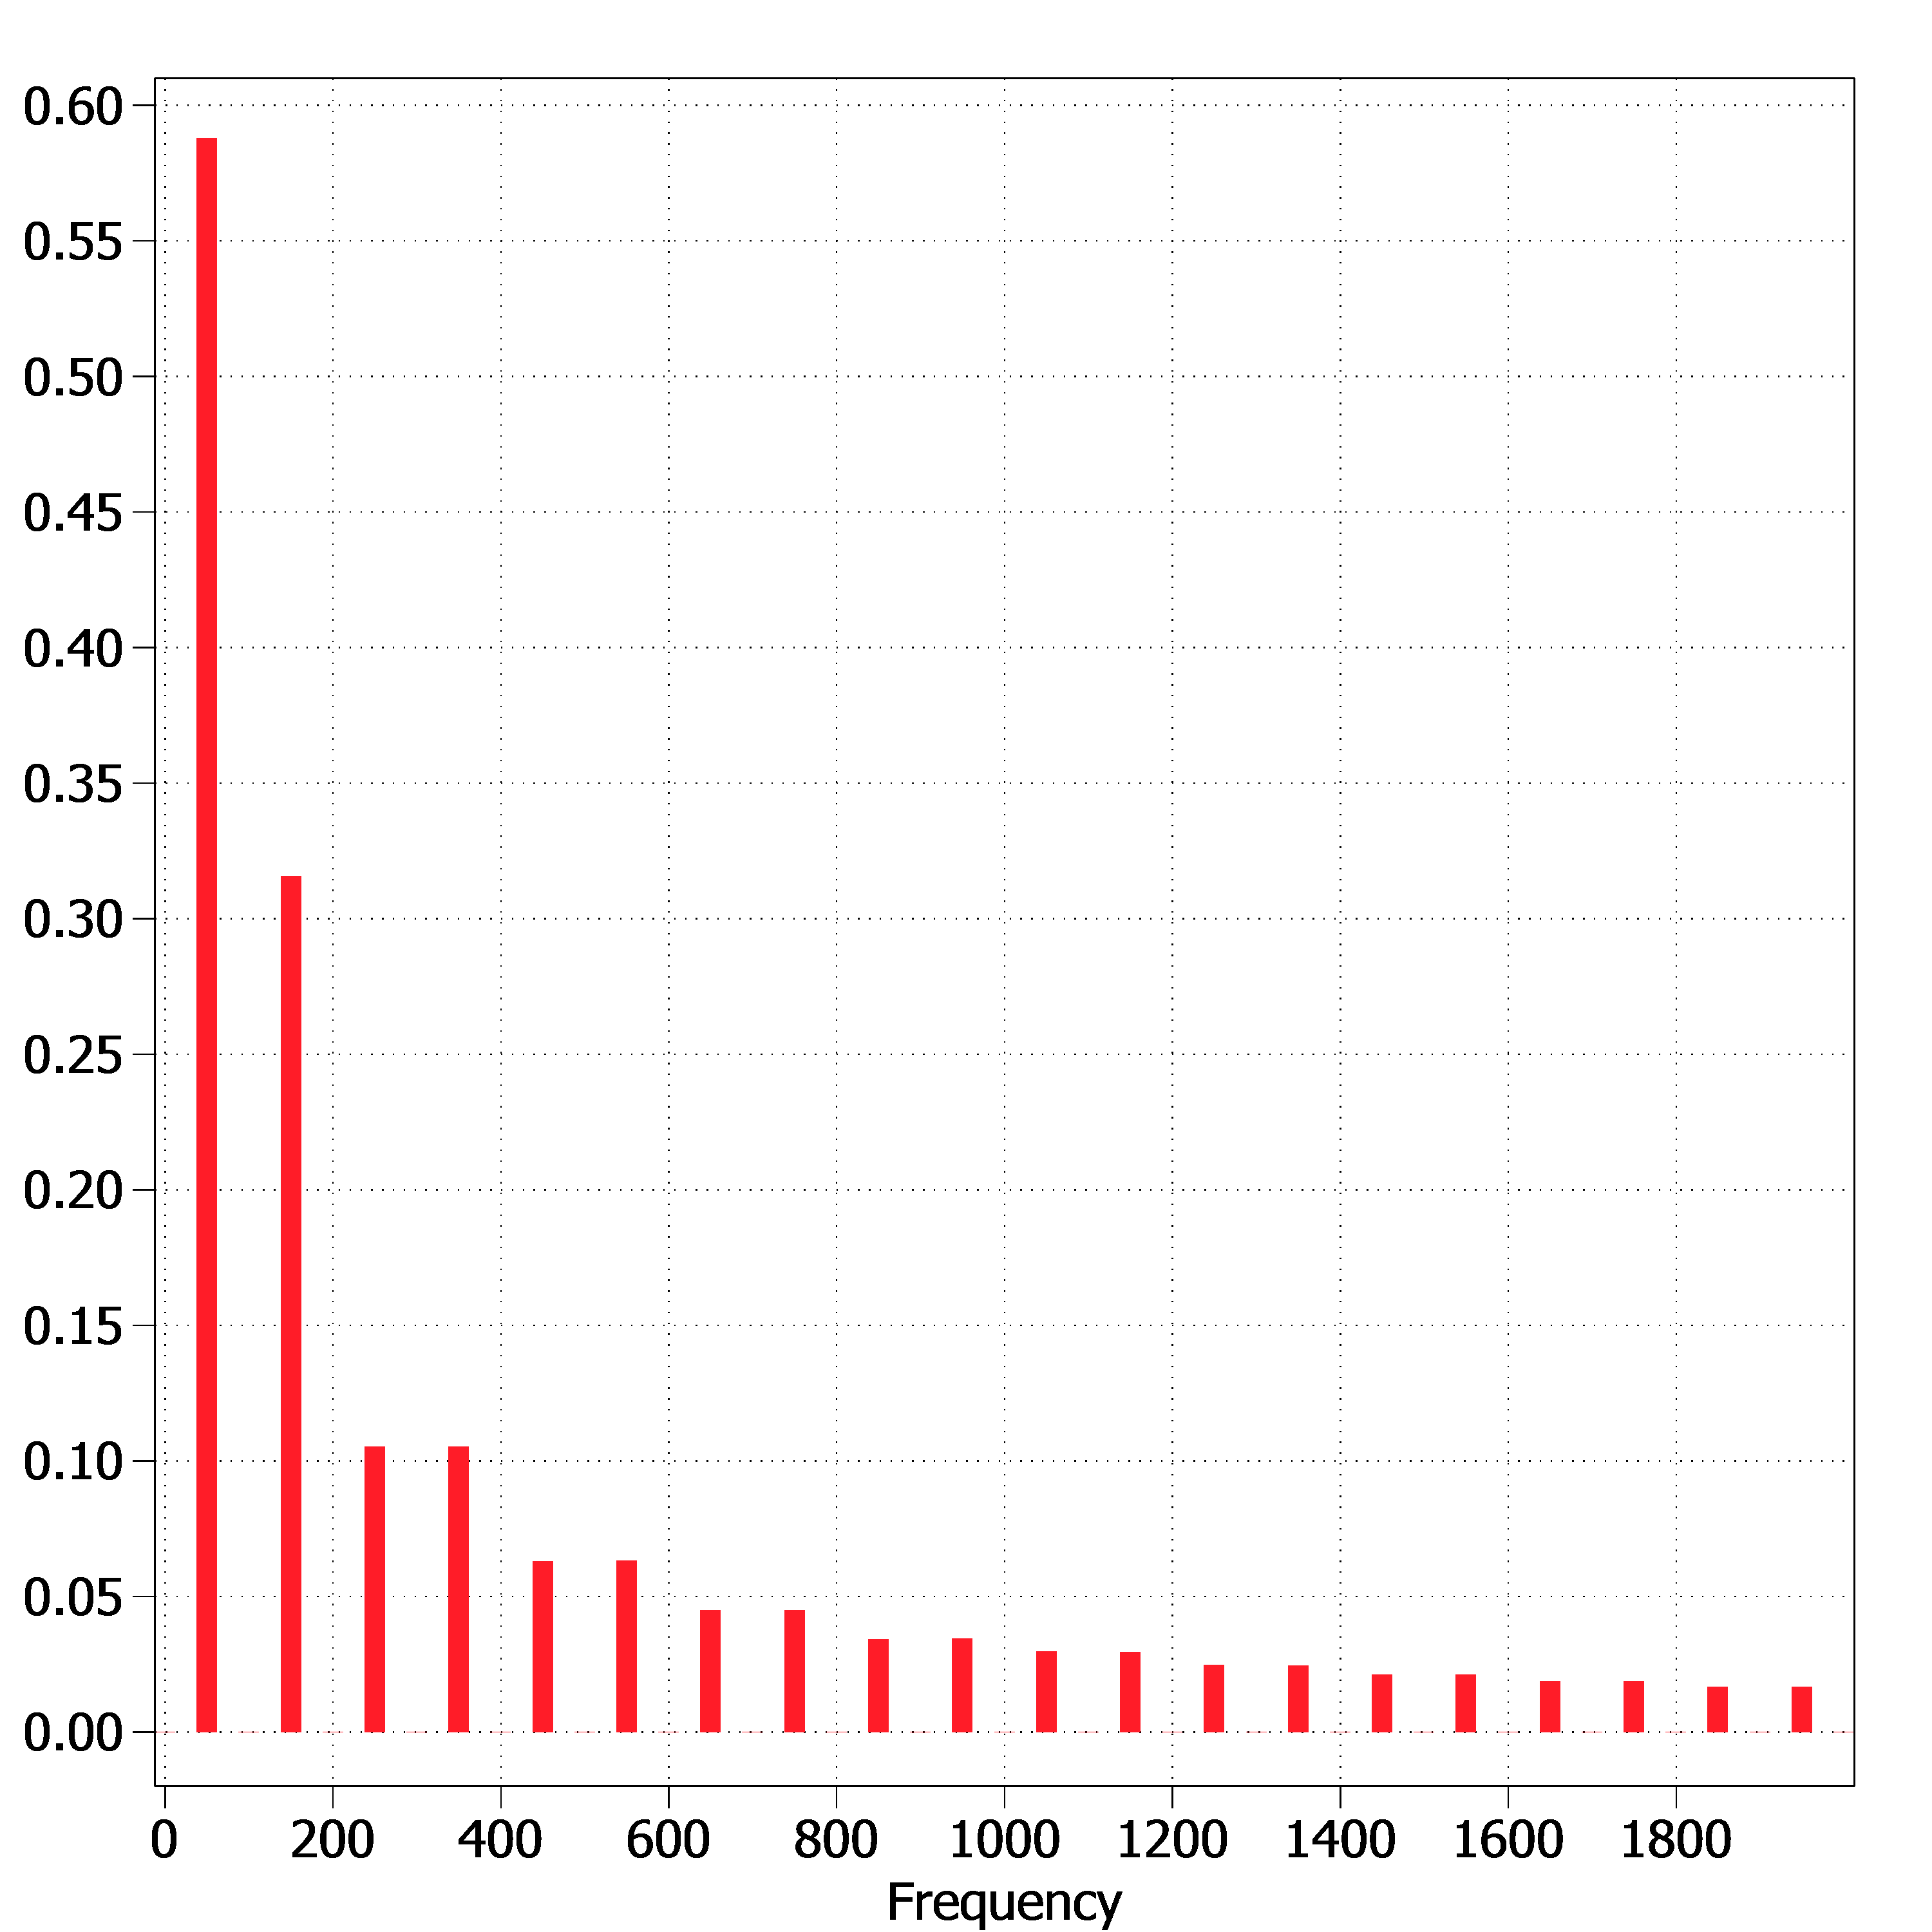
\includegraphics[width=0.43\linewidth]{plecs_phasenanschnitt_pi_2.png}\label{fig:plecs_Amplitudenspektrum_90}}
	\caption{Amplitudenspektrum Phasenanschnitt (a) 60\textdegree (b) 90\textdegree}
	\label{fig:plecs_Amplitudenspektrum}
\end{figure}


\subsubsection{Einphasige Schwingungspaketsteuerung mit Duty Cycle von 0.5 und 0.8}

Als Nächstes wird eine Simulation für die Schwingungspaketsteuerung aufgebaut, ersichtlich in den Abbildungen \ref{fig:plecs_Schwingungspakete}. Auch hier ist je ein Duty Cycle von 0.5, auf der Abbildung \ref{fig:plecs_Schwingungspaket_0_5}, beziehungsweise 0.8 auf der Abbildung \ref{fig:plecs_Schwingungspaket_0_8}, verwendet worden. So sind die Resultate mit den Resultaten mit der Matlab-Funktion vergleichbar. Andere Duty Cycle sind im Anhang im Kapitel \ref{sec:Vergleich_der_Resultate} ersichtlich. 
\begin{figure}[ht!]
	\centering
	\subfloat[][]{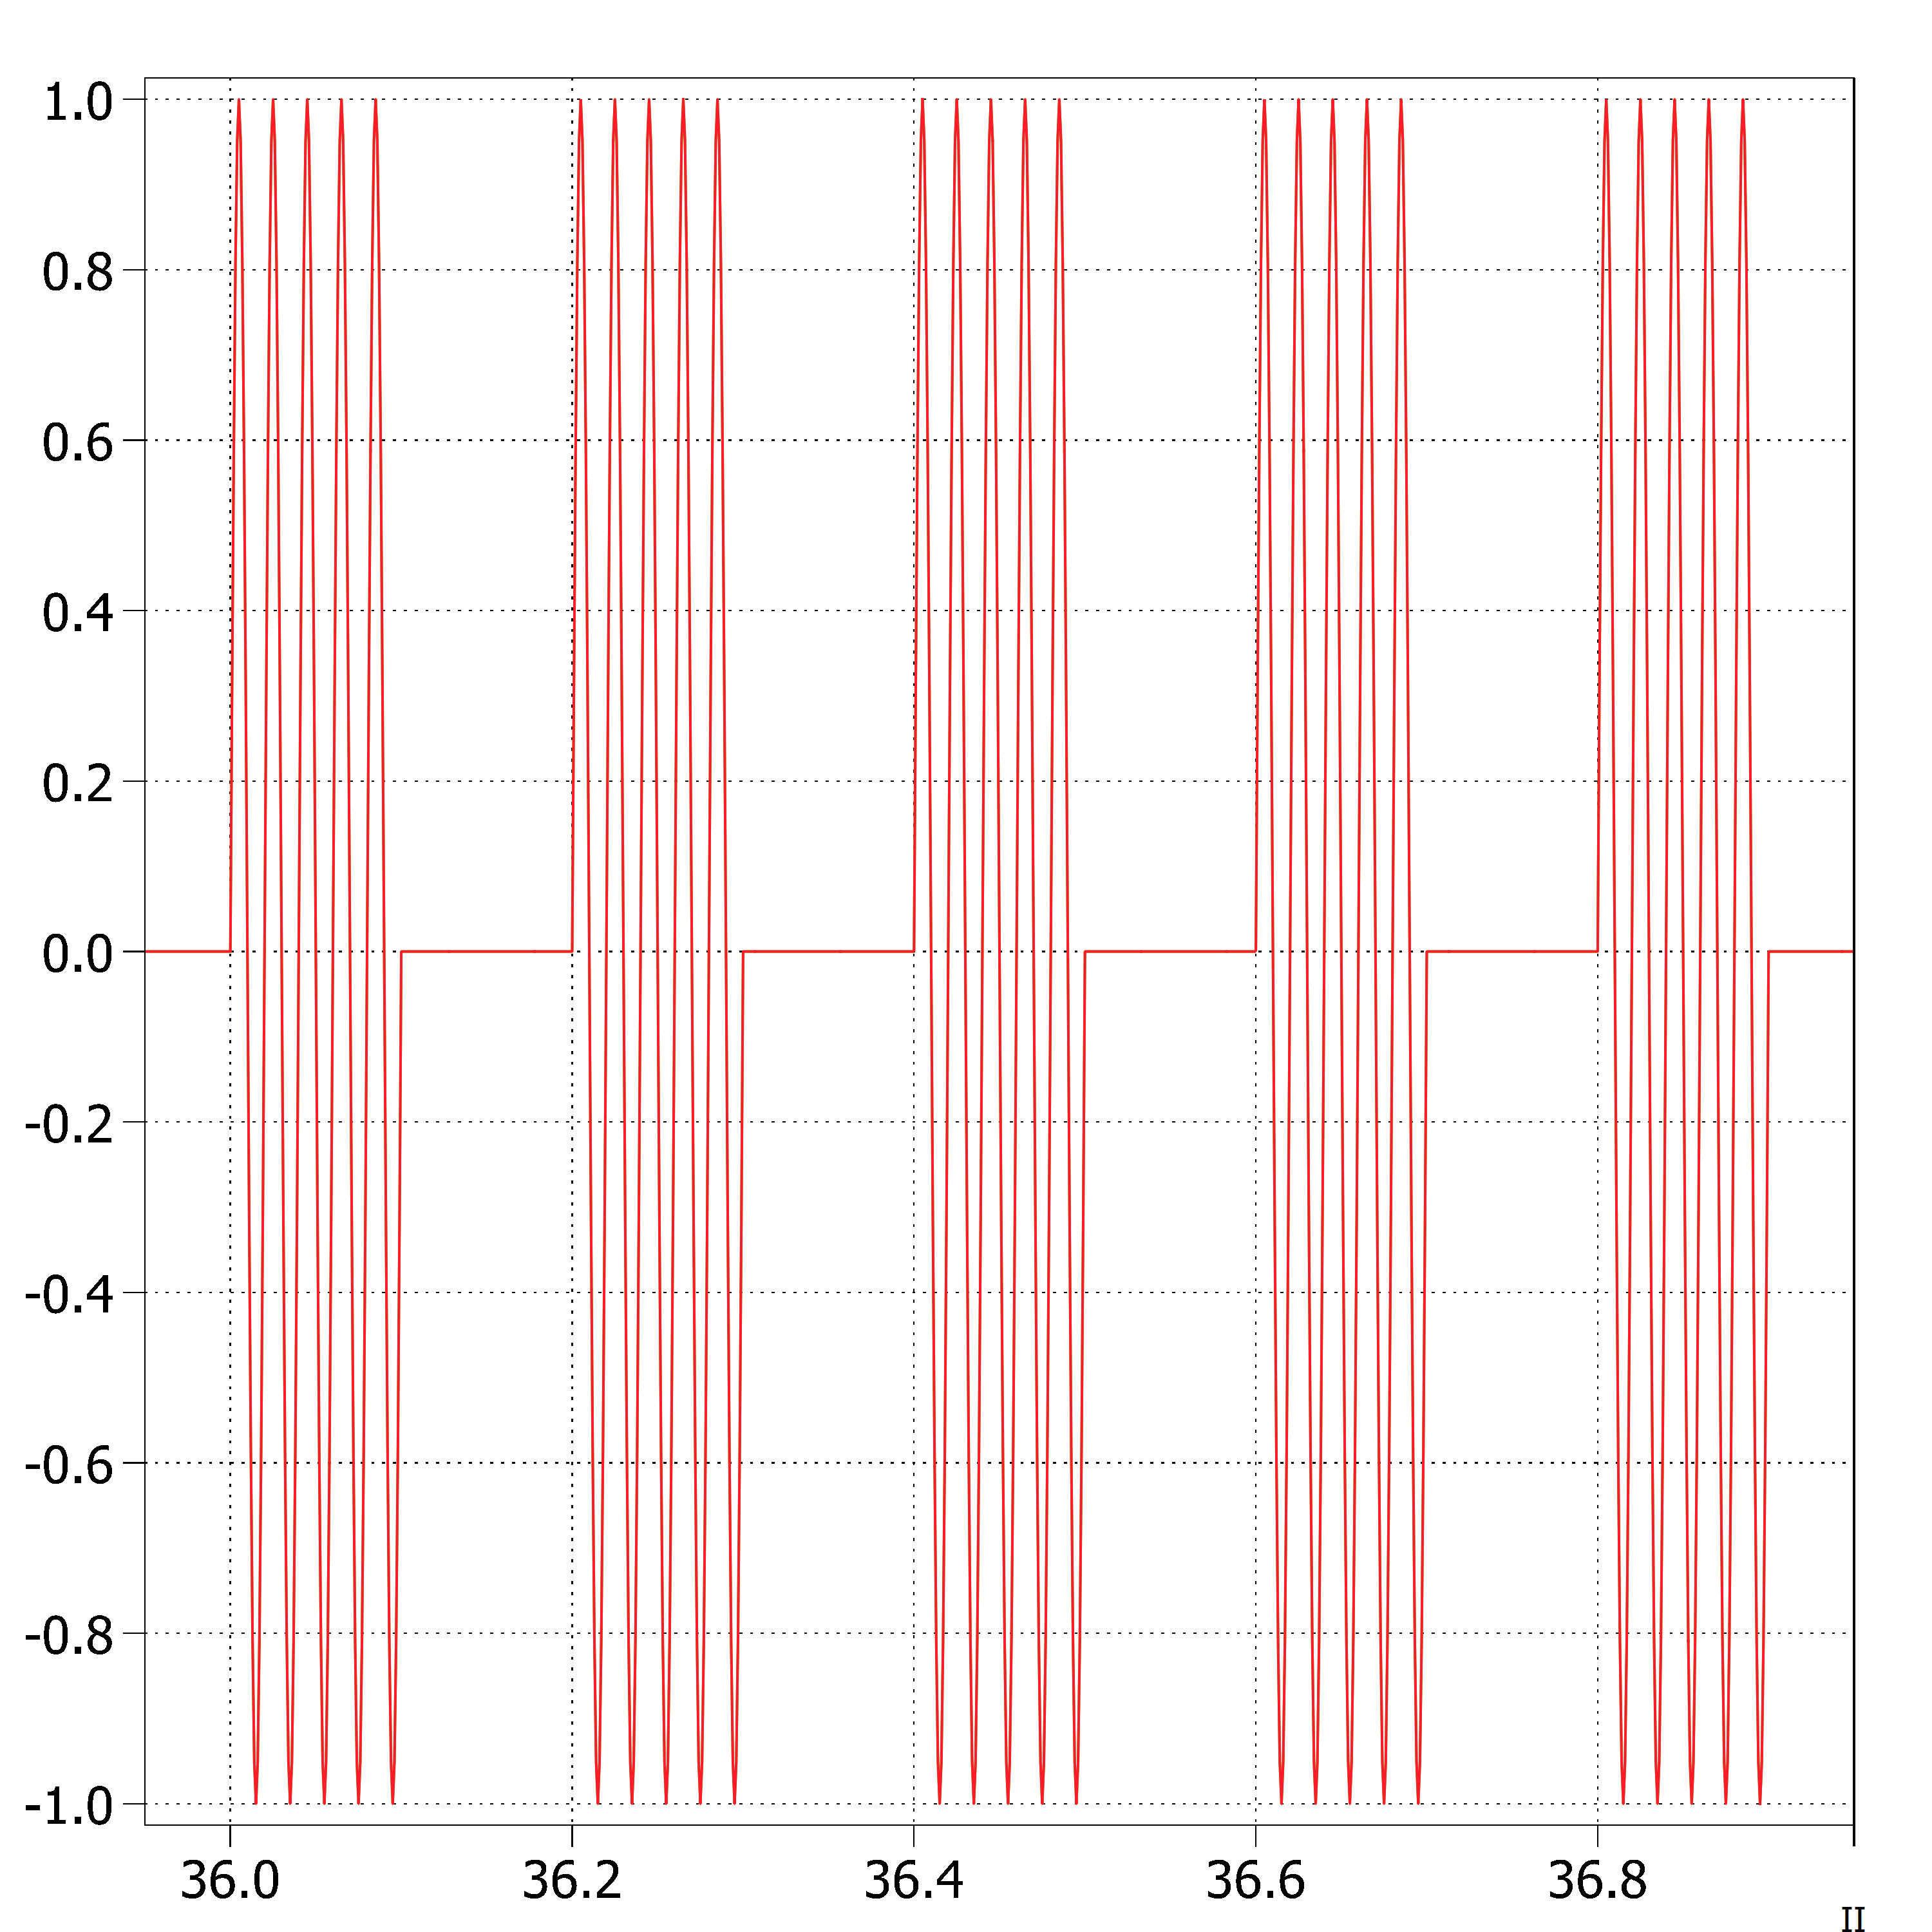
\includegraphics[width=0.45\linewidth]{plecs_schwingungspacket_0_5_schwingungen.PNG}\label{fig:plecs_Schwingungspaket_0_5}}\qquad
	\subfloat[][]{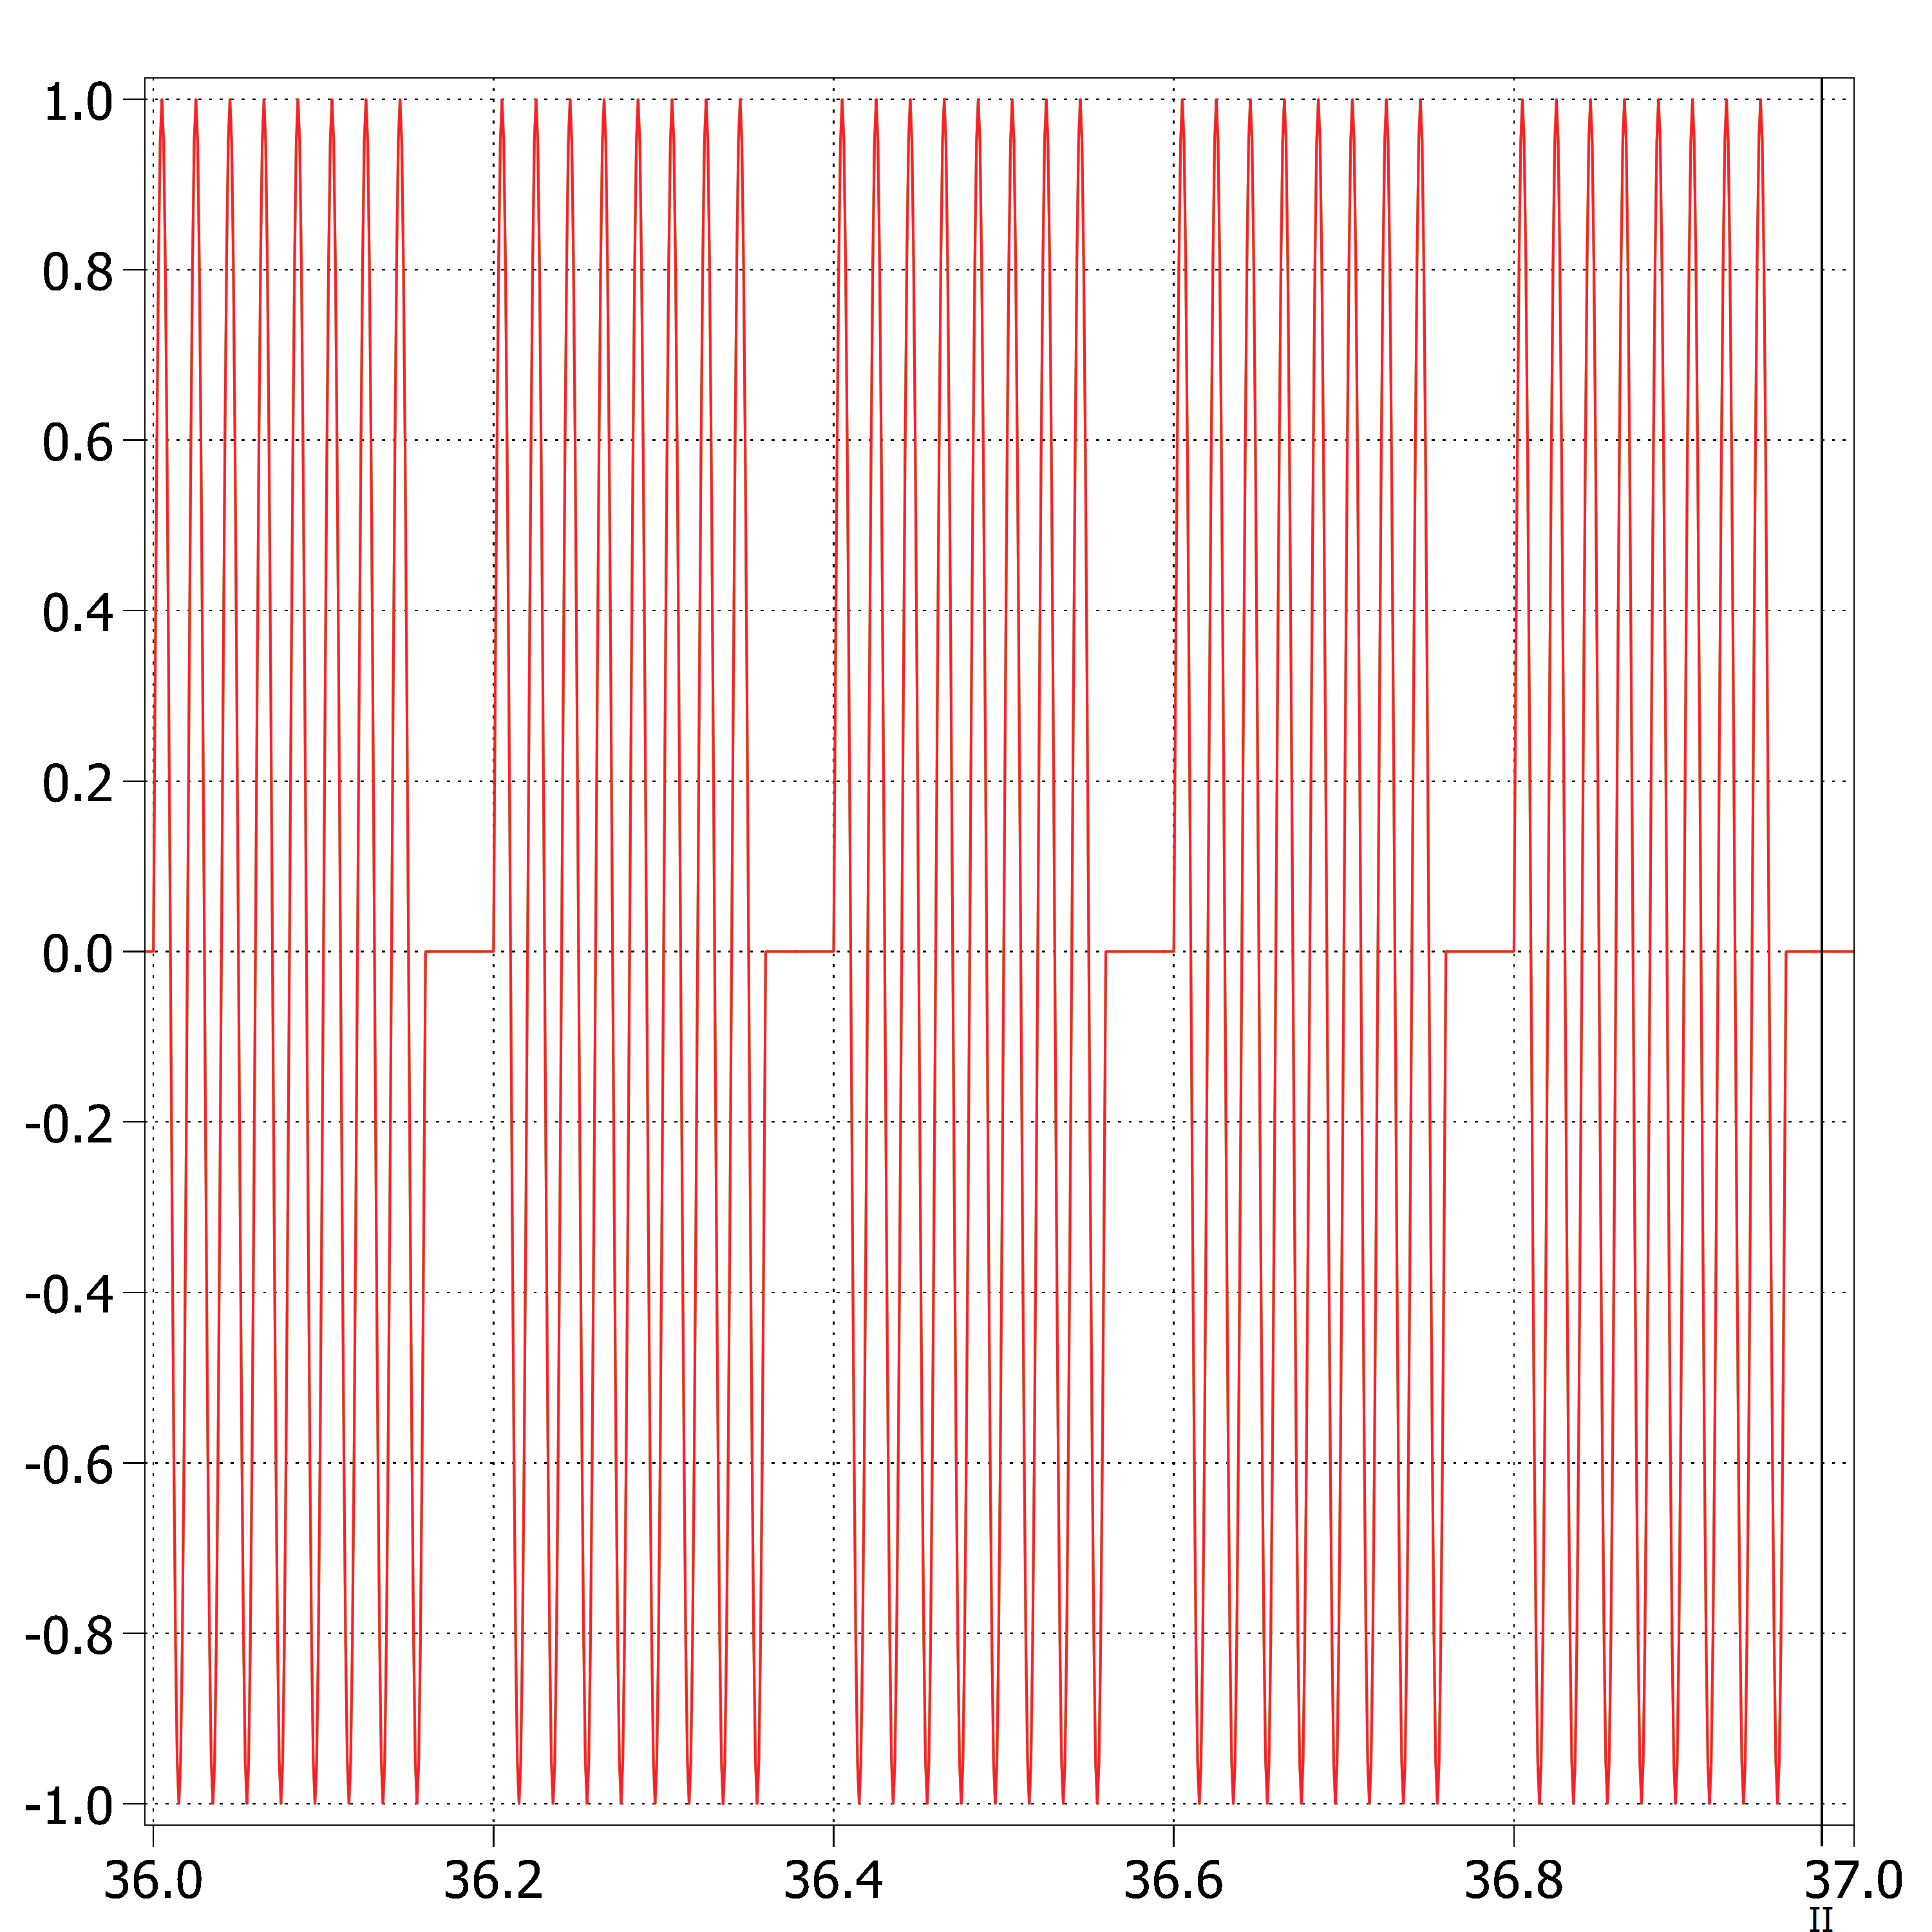
\includegraphics[width=0.45\linewidth]{plecs_schwingungspacket_0_8_schwingungen.PNG}\label{fig:plecs_Schwingungspaket_0_8}}
	\caption{Schwingungspaket mit einem Duty Cycle (a) 0.5 (b) 0.8}
	\label{fig:plecs_Schwingungspakete}
\end{figure}

\newpage
In der Abbildung \ref{fig:plecs_Schwingungspakete_Amplitudenspektrum_ 0_5_100_1000} ist das Amplitudenspektrum des Schwingungspaketes mit einem Duty Cycle von 0.5 dargestellt. Auf der linken Seite der Abbildung \ref{fig:plecs_Schwingungspaket_0_5_100} erkennt man das bekannte Spektrum von 0 - 100 Hz mit den subharmonischen Werten unterhalb von 50 Hz und den zwischenharmonischen Schwingungen von 50 - 100 Hz. In Abbildung  \ref{fig:plecs_Schwingungspaket_0_5_1000} erweiterte man das Spektrum bis zu 1000 Hz. Auch hier ist eine optische Ähnlichkeit zur  Matlab-Funktion ersichtlich.
  
\begin{figure}[ht!]
	\centering
	\subfloat[][]{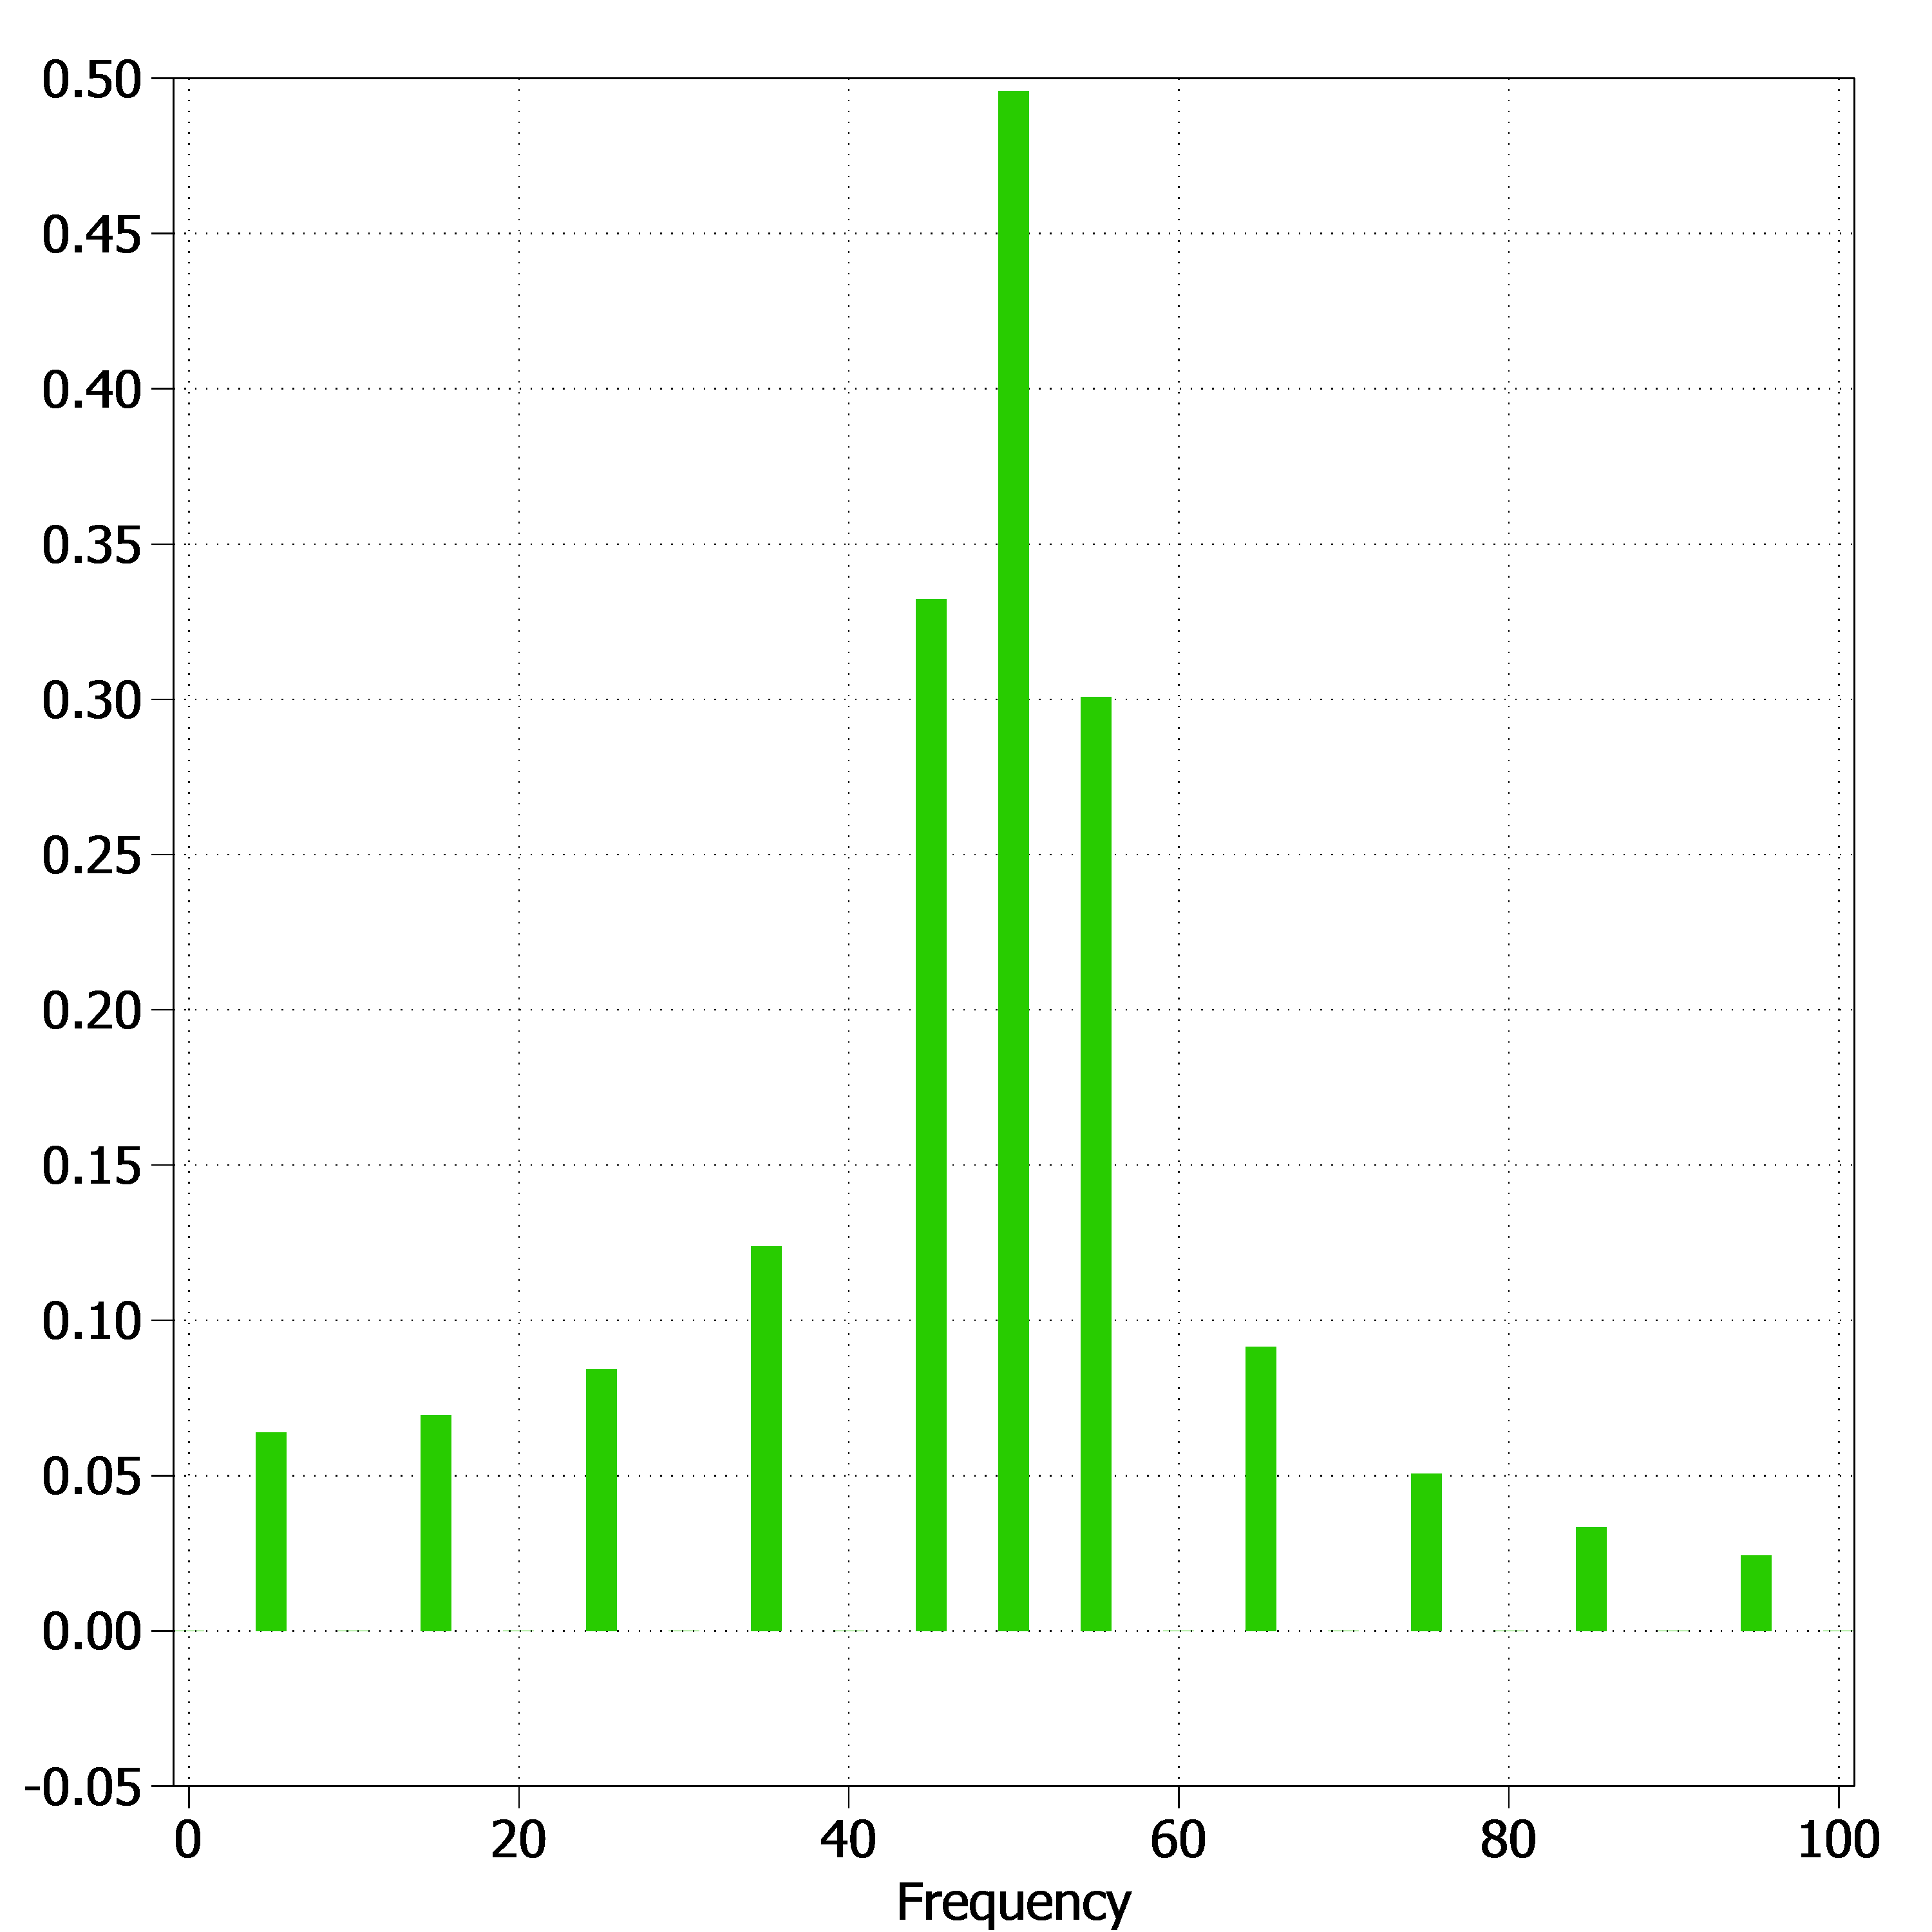
\includegraphics[width=0.45\linewidth]{plecs_schwingungspacket_0_5_100.PNG}\label{fig:plecs_Schwingungspaket_0_5_100}}\qquad
	\subfloat[][]{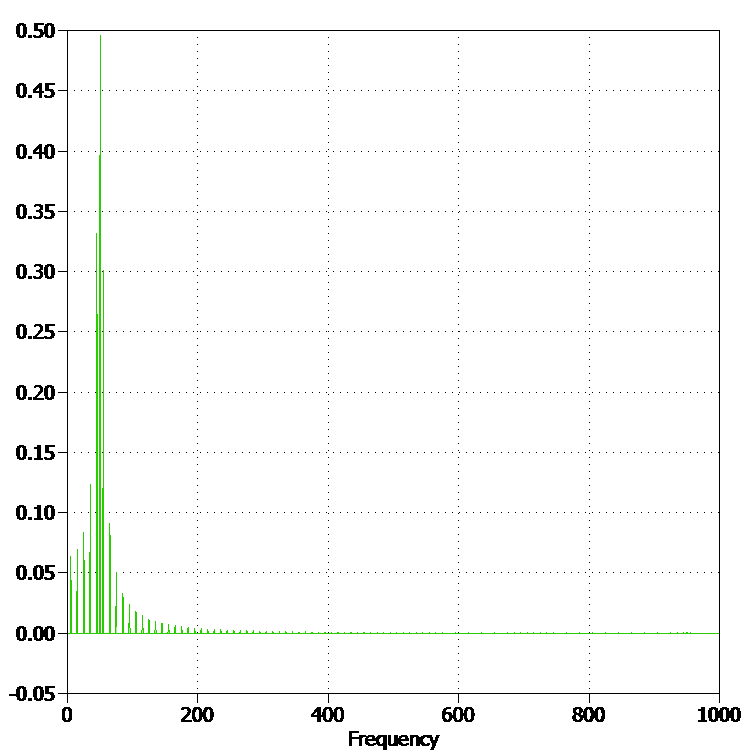
\includegraphics[width=0.45\linewidth]{plecs_schwingungspacket_0_5_1000.PNG}\label{fig:plecs_Schwingungspaket_0_5_1000}}
	\caption{Amplitudenspektrum mit einem Duty Cycle 0.5 von (a) 0 - 100 Hz (b) 0 - 1000 Hz}
	\label{fig:plecs_Schwingungspakete_Amplitudenspektrum_ 0_5_100_1000}
\end{figure}

\newpage
Vollständigkeitshalber ist das Gleiche noch mit einem Duty Cycle von 0.8 realisiert. Auch hier ist das Spektrum, in der linken Abbildung \ref{fig:plecs_Schwingungspaket_0_8_100} mit einer Frequenz von 0 - \SI{100}{Hz} und in der rechten Abbildung \ref{fig:plecs_Schwingungspaket_0_8_1000} bis \SI{1000}{Hz}, dargestellt. 


\begin{figure}[ht!]
	\centering
	\subfloat[][]{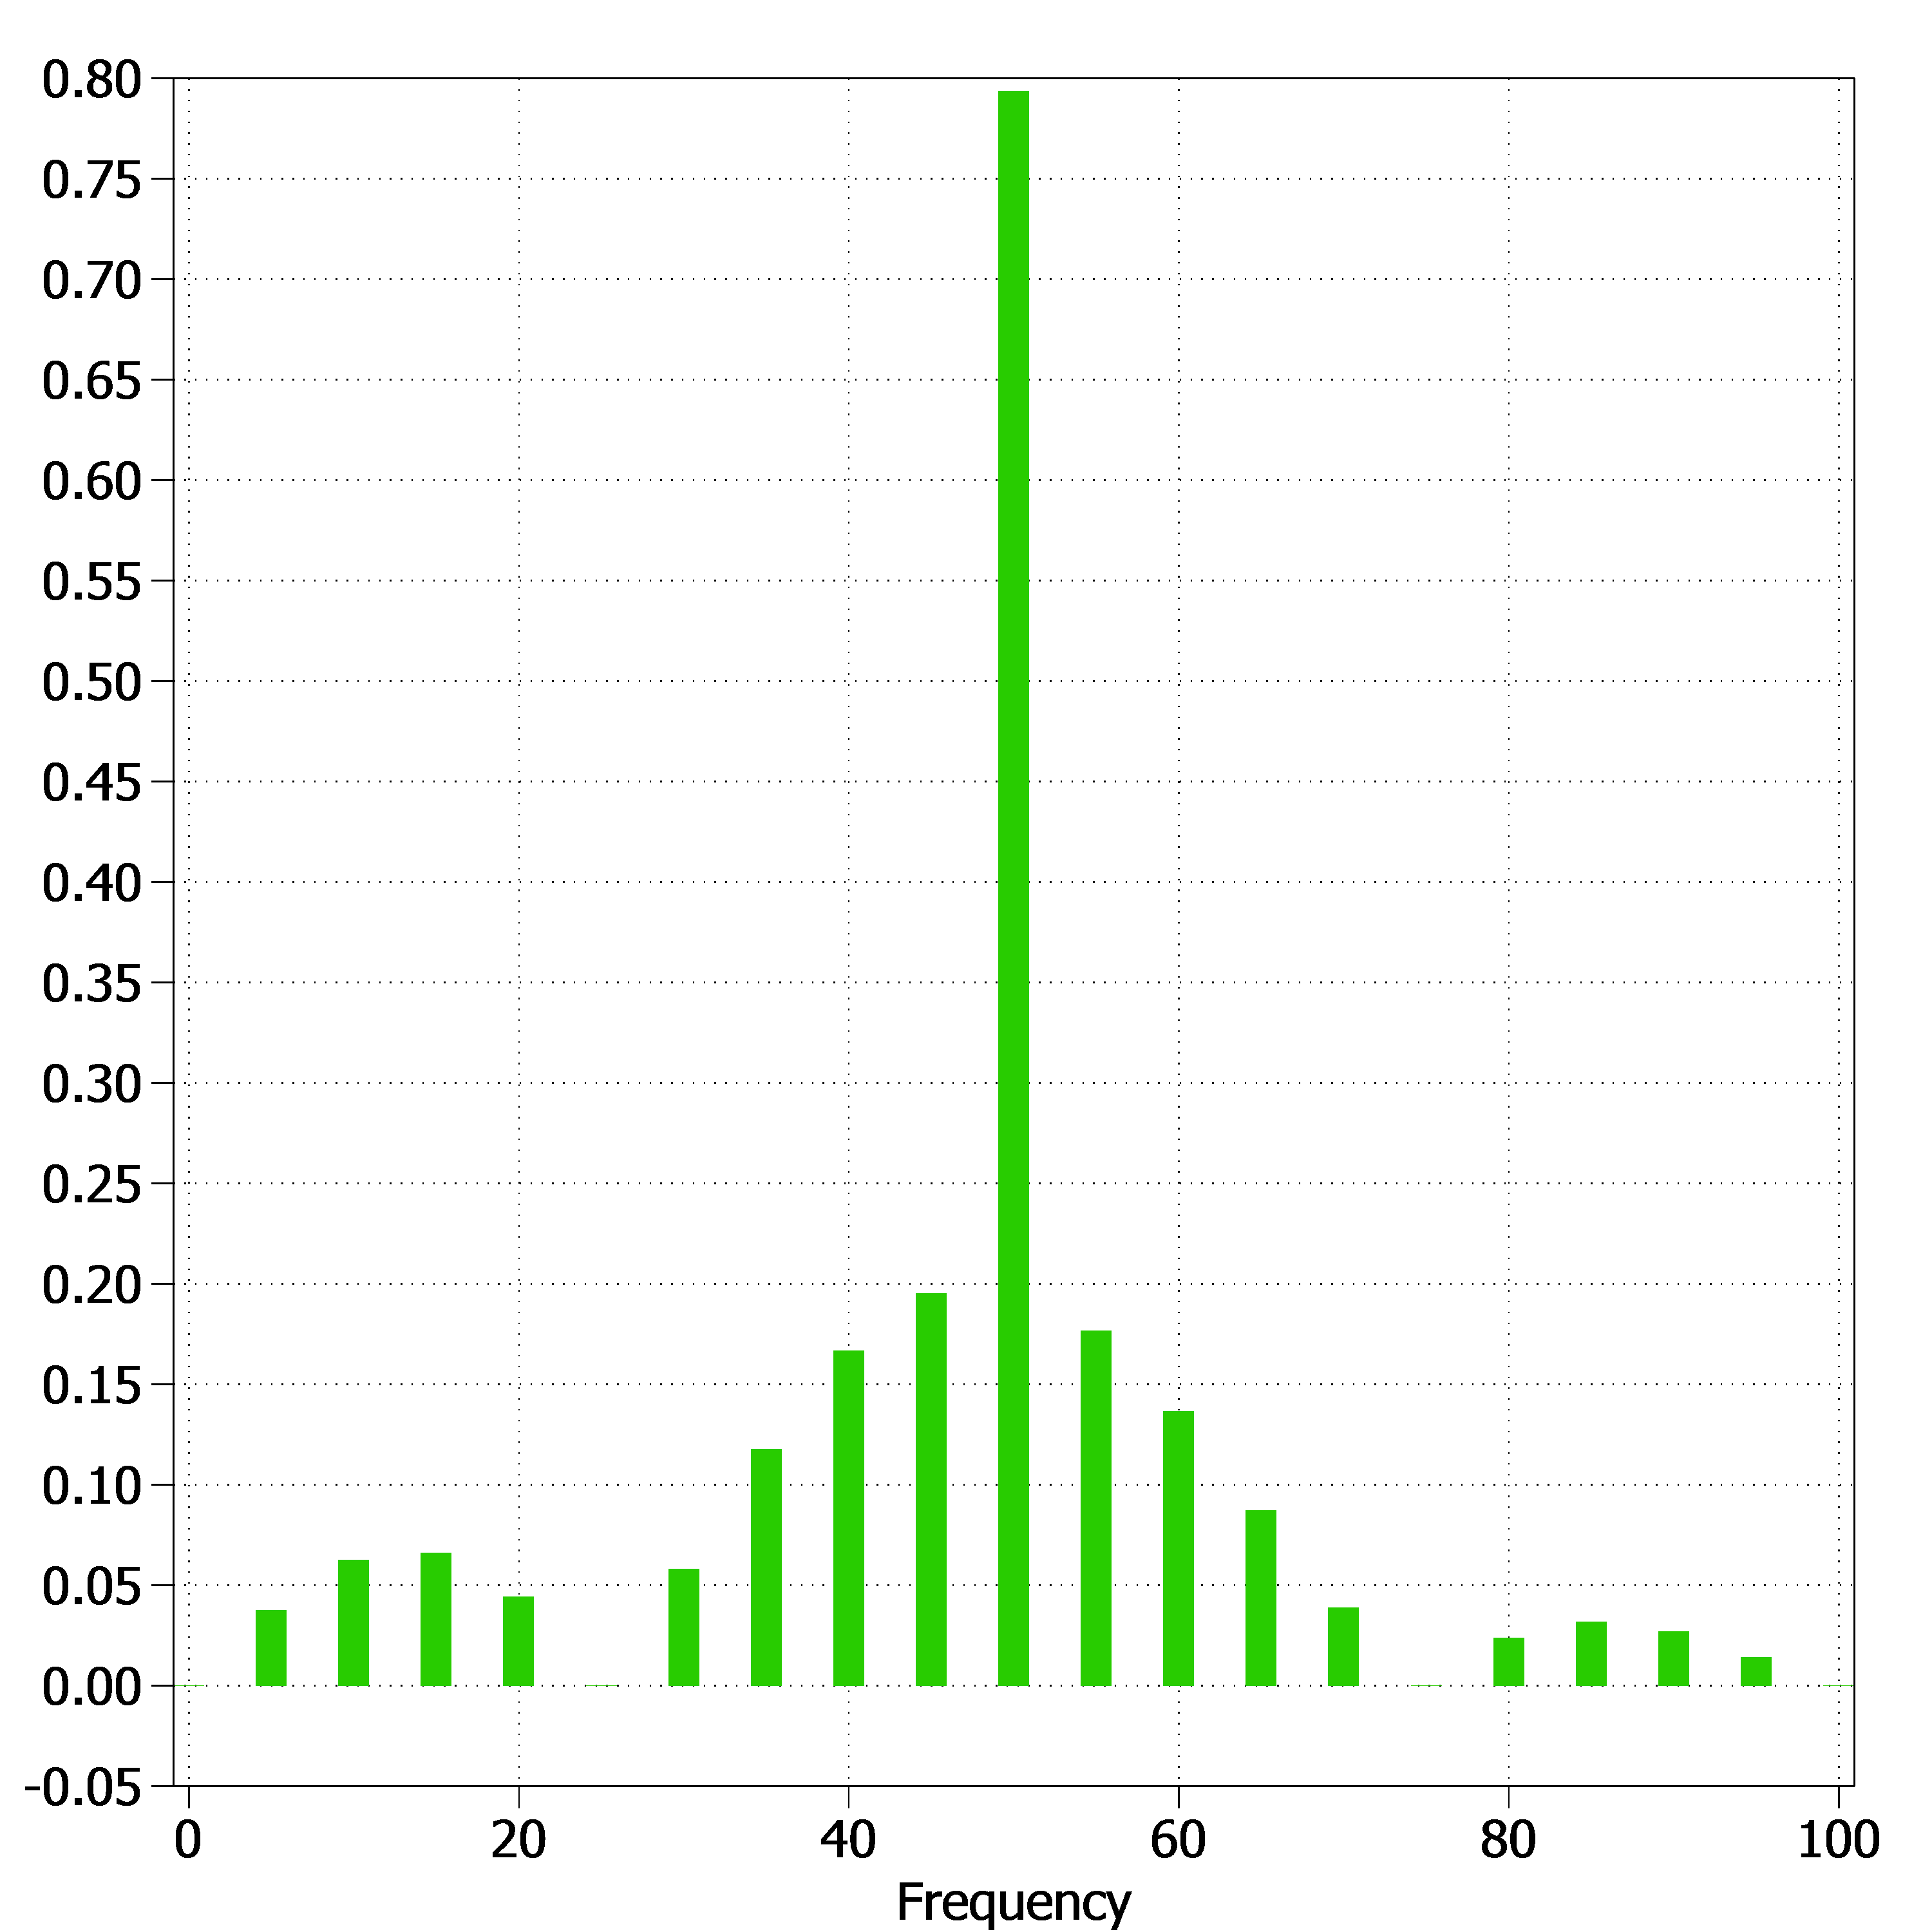
\includegraphics[width=0.45\linewidth]{plecs_schwingungspacket_0_8.PNG}\label{fig:plecs_Schwingungspaket_0_8_100}}\qquad
	\subfloat[][]{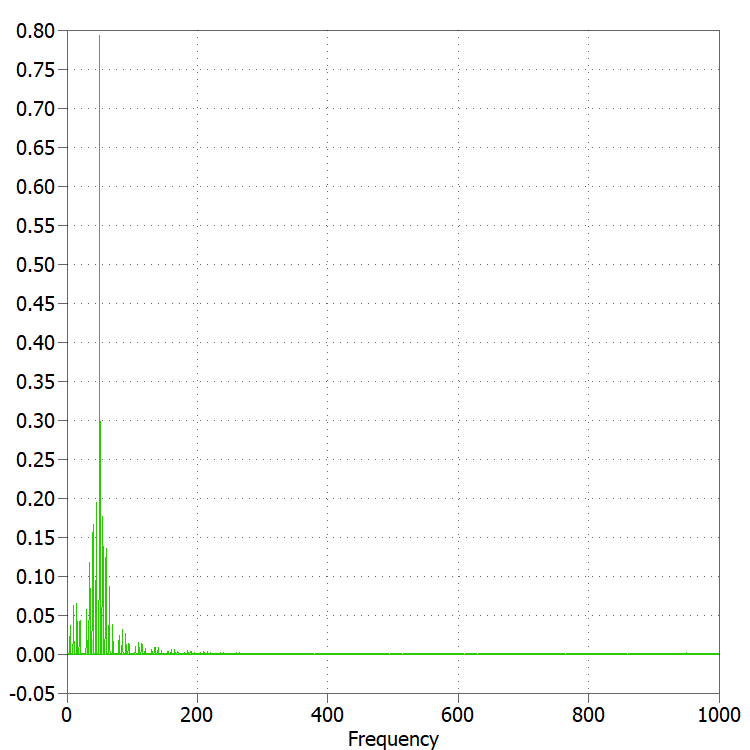
\includegraphics[width=0.45\linewidth]{plecs_schwingungspacket_0_8_1000.PNG}\label{fig:plecs_Schwingungspaket_0_8_1000}}
	\caption{Amplitudenspektrum mit einem Duty Cycle 0.8 von (a) 0 - \SI{100}{Hz} (b) 0 - \SI{1000}{Hz}}
	\label{fig:plecs_Schwingungspakete_Amplitudenspektrum_ 0_8_100_1000}
\end{figure}

Zum Schluss ist das lineare absolute Spektrum der beiden Duty Cycles, 0.5 in der Abbildung \ref{fig:plecs_Schwingungspaket_0_5_absolut_log} und 0.8 in der Abbildung \ref{fig:plecs_Schwingungspaket_0_8_absolut_log}, veranschaulicht. Damit man die Grafiken mit der Matlab-Simulation vergleichen kann, wird das Spektrum bis zu einer Frequenz von \SI{100}{Hz} angezeigt. Auch hier erkennt man eine optische Ähnlichkeit zur Matlab-Simulation. 


\begin{figure}[ht!]
	\centering
	\subfloat[][]{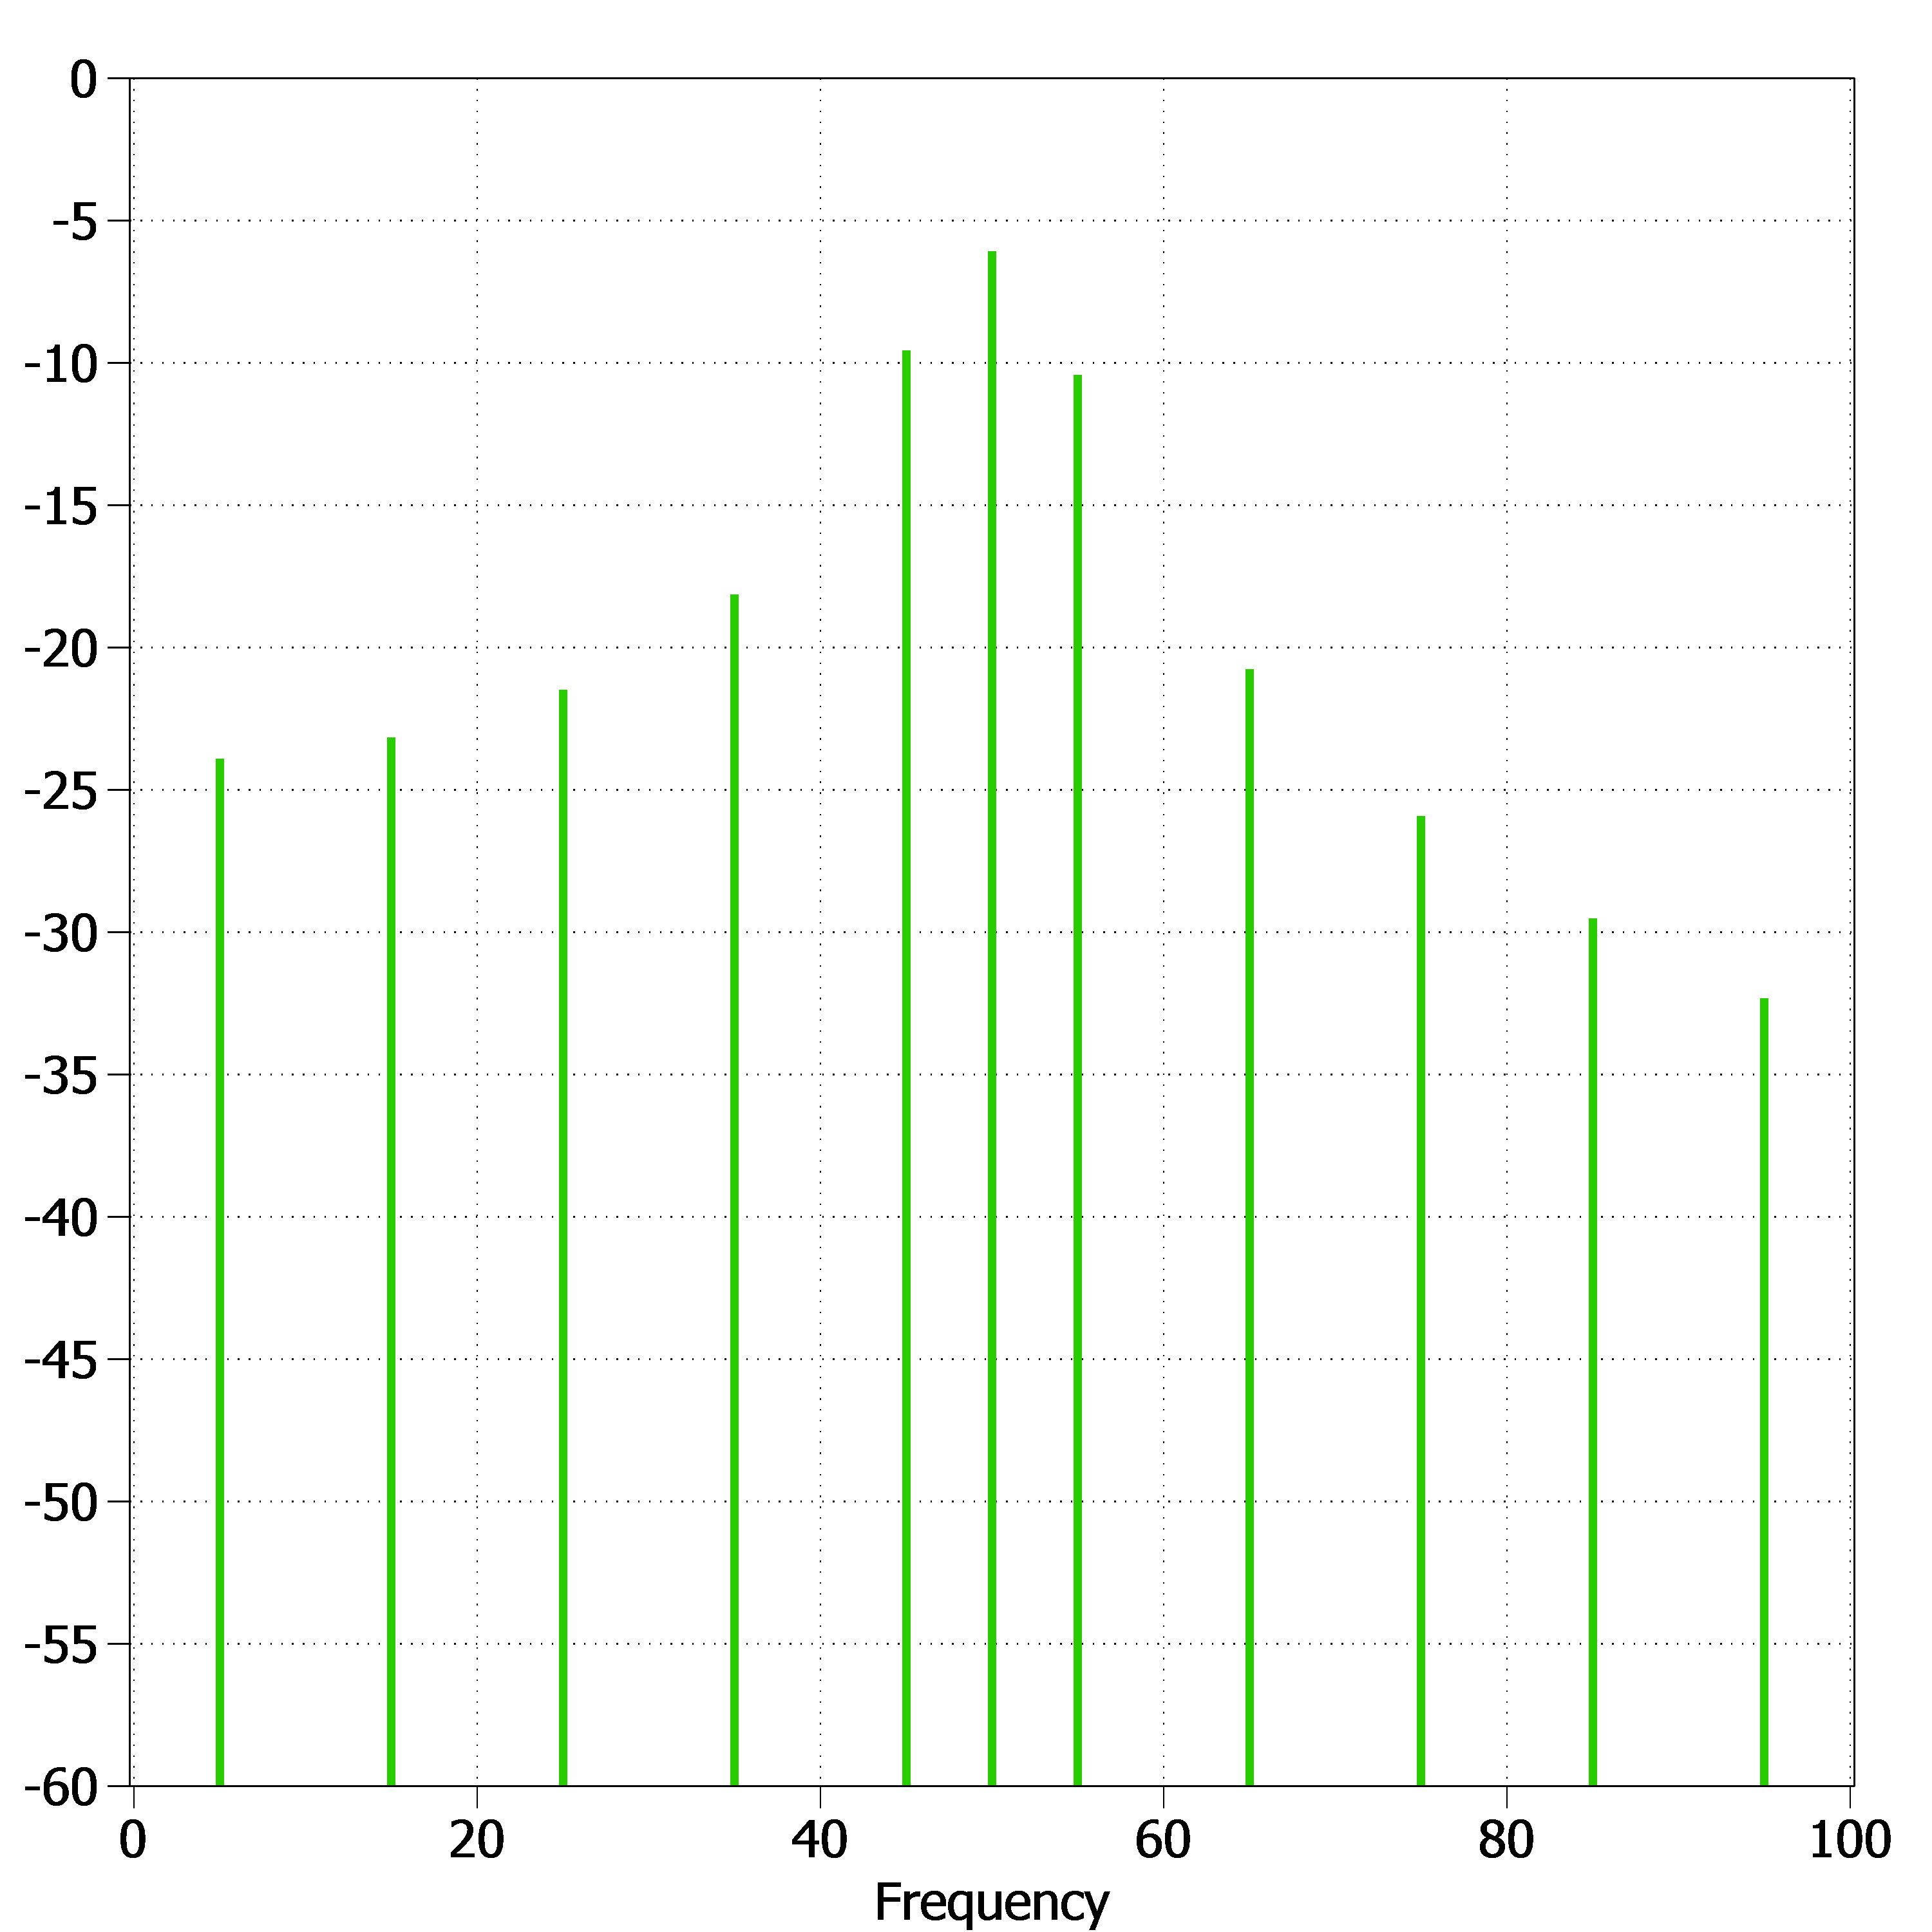
\includegraphics[width=0.45\linewidth]{plecs_schwingungspacket_0_5_absolut_log.PNG}\label{fig:plecs_Schwingungspaket_0_5_absolut_log}}\qquad
	\subfloat[][]{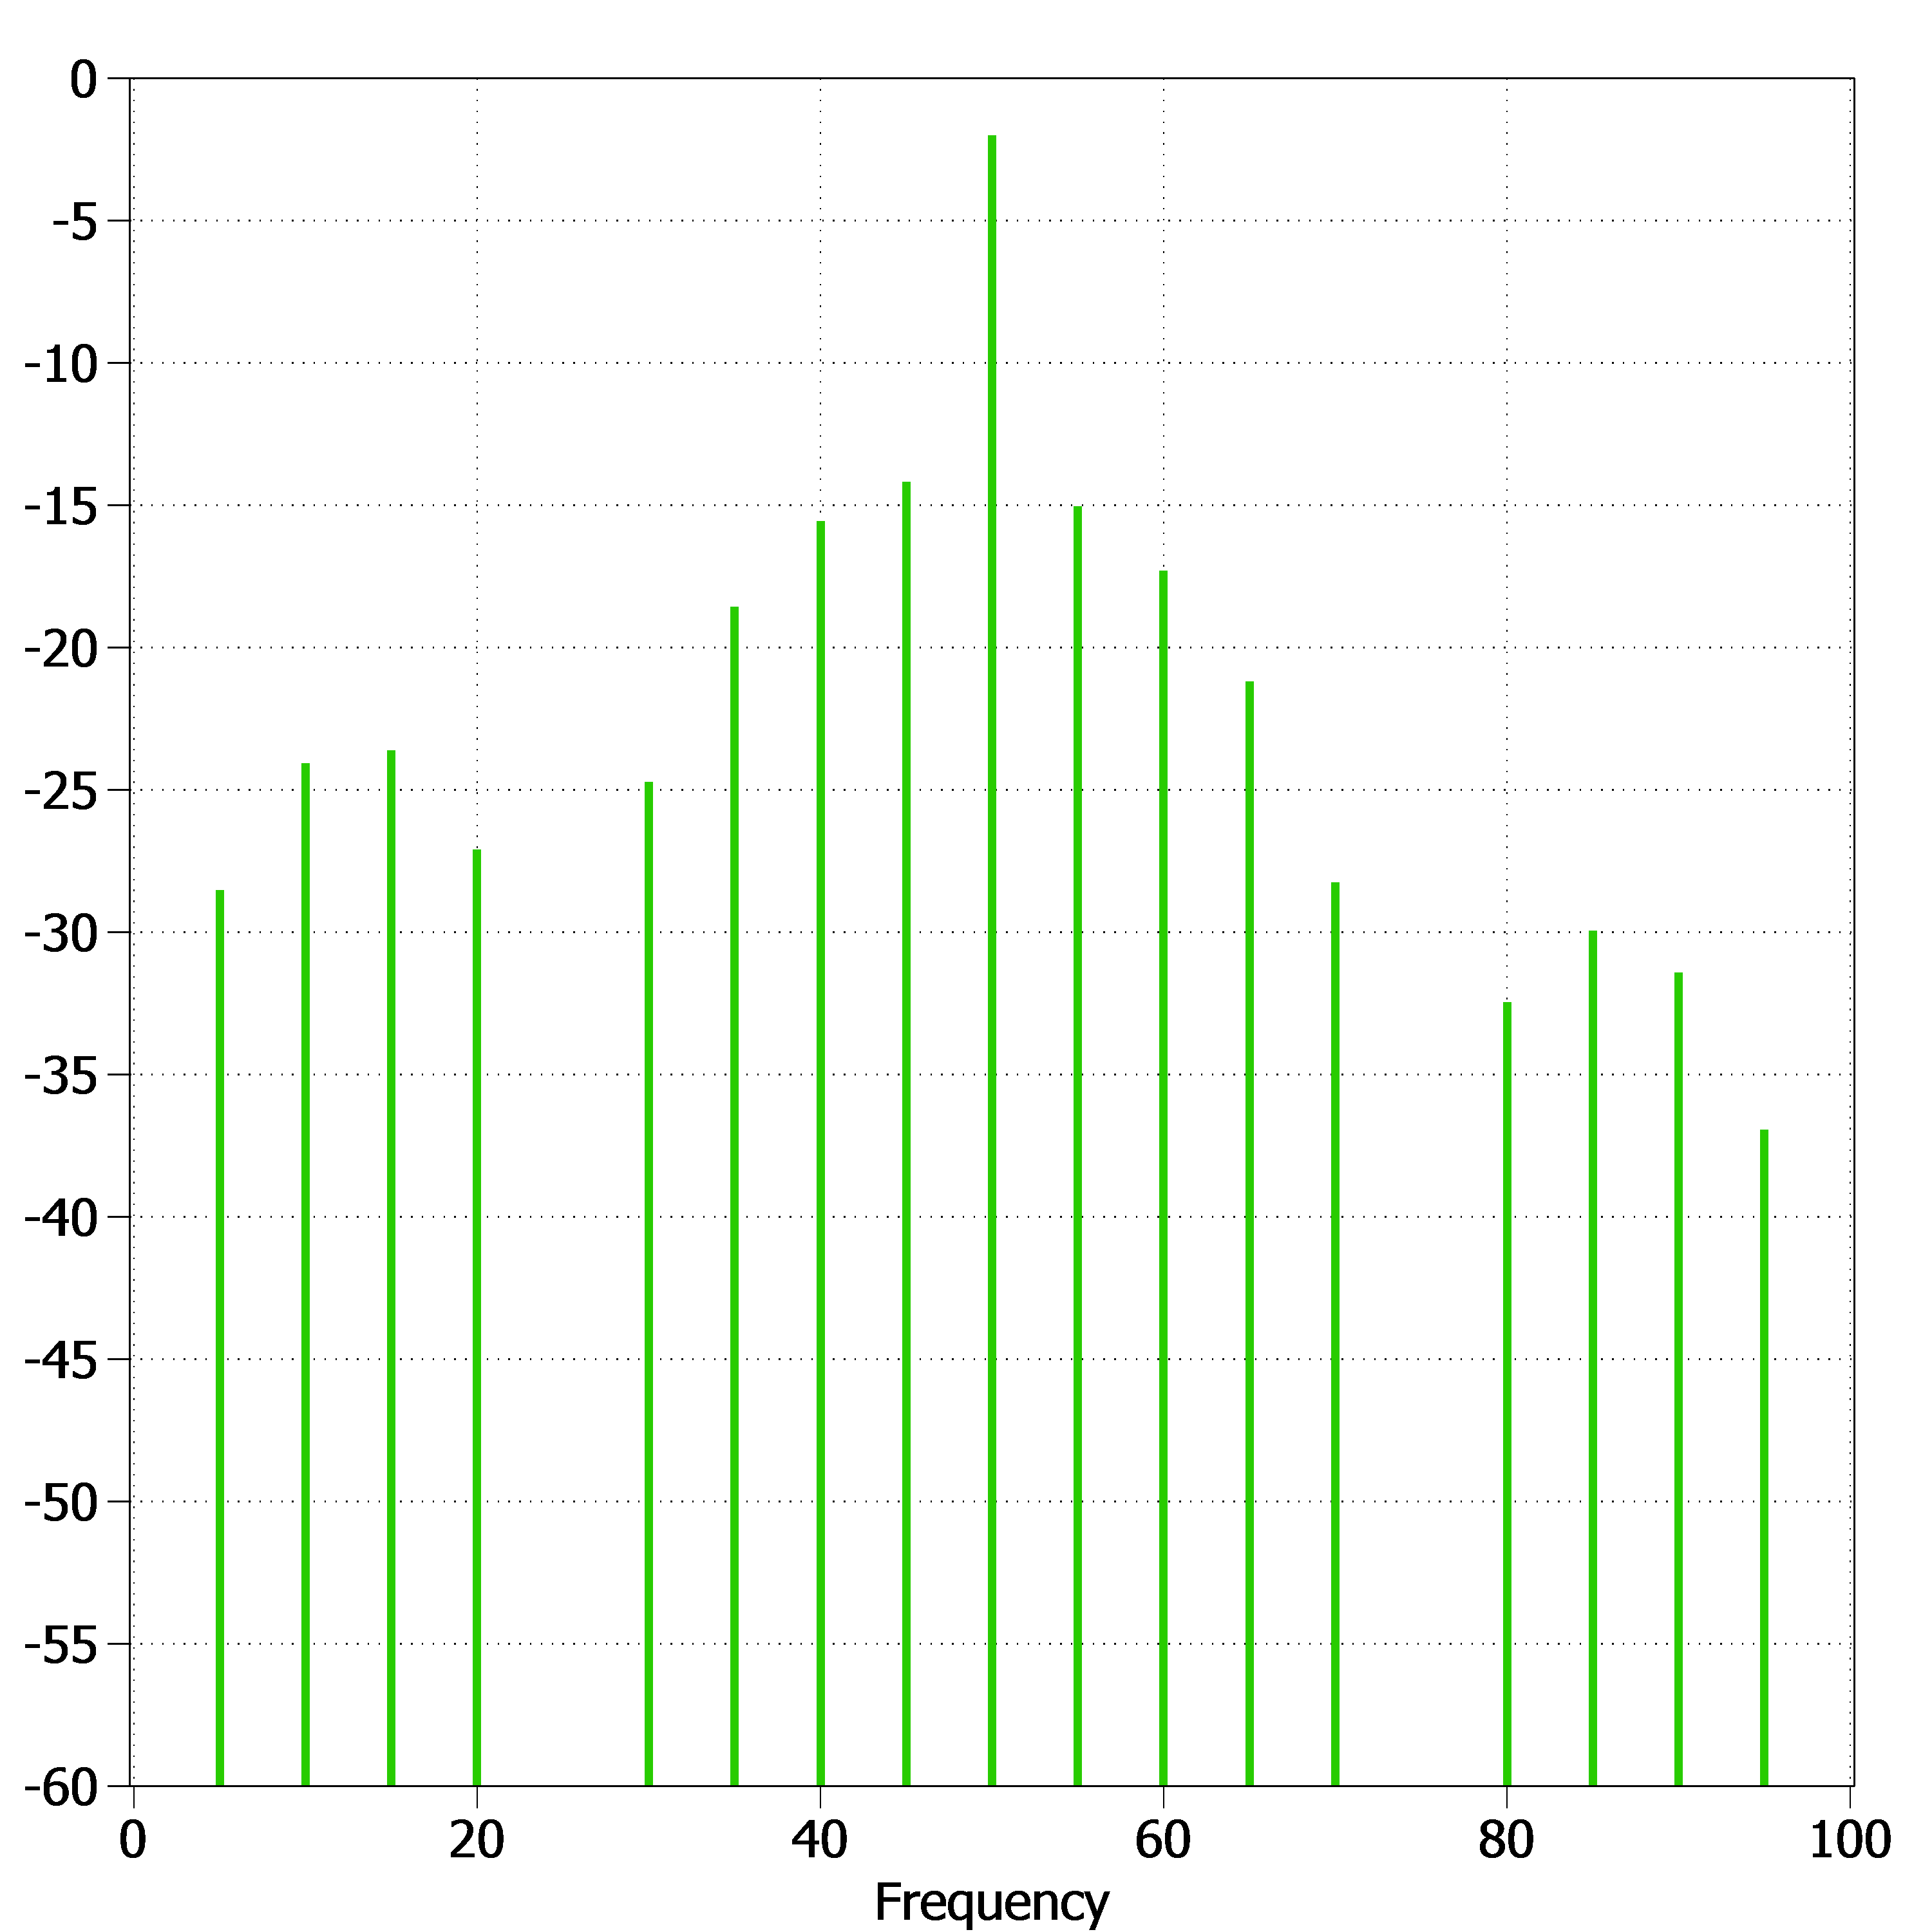
\includegraphics[width=0.45\linewidth]{plecs_schwingungspacket_0_8_absolut_log.PNG}\label{fig:plecs_Schwingungspaket_0_8_absolut_log}}
	\caption{Lineares absolutes Spektrum mit einem Duty Cycle von (a) 0.5 (b) 0.8}
	\label{fig:plecs_Schwingungspakete_absolut log}
\end{figure}

\newpage
\subsubsection{Vergleich der einphasigen Resultate mit Plecs und Matlab} \label{sec:Vergleich_Plecs_Matlab}
Optisch betrachtet, sehen die Resultate der beiden einphasigen Simulationen sehr ähnlich aus. Um jedoch eine konkrete Bestätigung der Analyse zu erhalten, wurden alle Werte der einphasigen Simulationen nummerisch und visuell miteinander verglichen. Man erkannte, dass die meisten gegenübergestellten Werte eine Abweichung von unter 1\% haben. Dies Abweichung entsteht, da man die Auflösung der Plecs-Simulation bewusst niedriger eingestellt hat, um die Berechnungszeit der Funktion zu verkürzen. Diese Abweichung konnte daher der Auflösung zugeschrieben werden. Die Resultaten sind gleichwohl für den Vergleich mit den Matlabwerten brauchbar. In der Abbildung \ref{fig:Amplitudenspektrum mit Phasenwinkel 90grad} ist der Vergleich des Amplitudenspektrums mit einem Phasenanschnittswinkel von 90\textdegree\hspace{0.02cm} ersichtlich. Die anderen Aufnahmen sind optisch und nummerisch im Anhang im Kapitel \ref{sec:Vergleich_der_Resultate} dargestellt.


\begin{figure}[ht!]
	\centering
	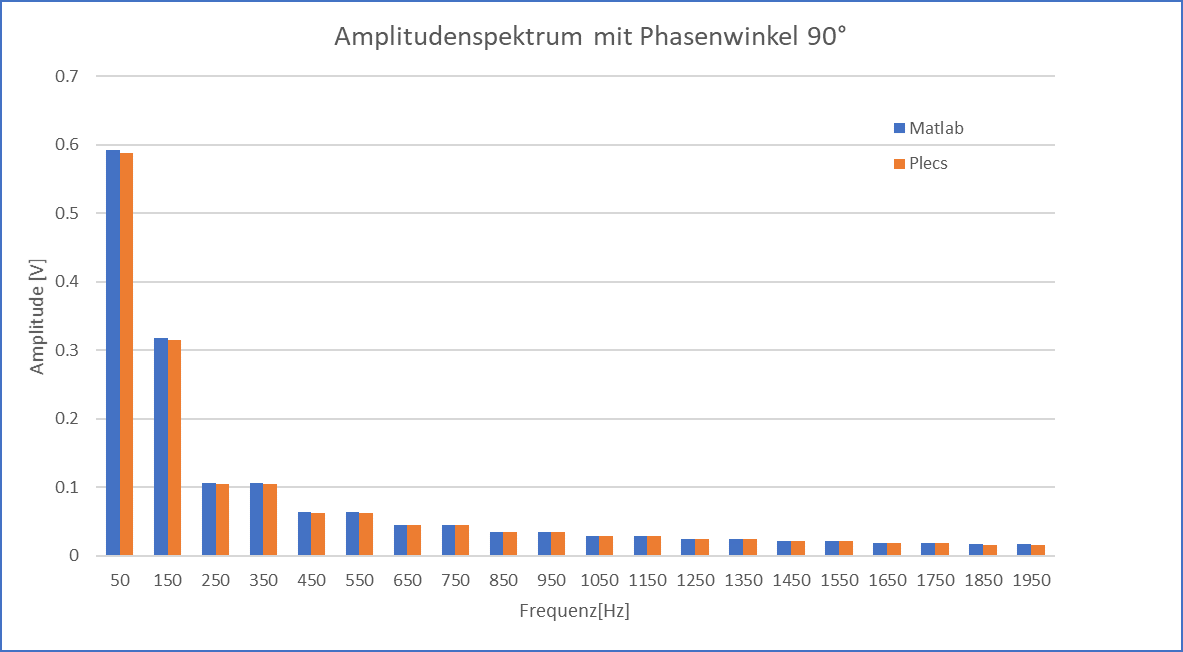
\includegraphics[scale=0.55]{Vergleich_Amplitudenspektrum_mit_Phasenwinkel_90.png}	
	\caption{Vergleich des Amplitudenspektrums mit Phasenwinkel 90\textdegree}
	\label{fig:Amplitudenspektrum mit Phasenwinkel 90grad}
\end{figure}


\subsubsection{Dreiphasige Phasenanschnittsteuerung mit 60\textdegree\hspace{0.02cm} und 90\textdegree}


Folgende Abbildungen \ref{fig:dreiphasige_Phasenanschnittsteuerung_mit_60} und \ref{fig:dreiphasige_Phasenanschnittsteuerung_mit_90} beinhalten die Simulation der dreiphasigen Phasenanschnittsteuerung, mit den bekannten Winkeln von 60\textdegree\hspace{0.02cm} und 90\textdegree\hspace{0.02cm}.
In den Abbildungen \ref{fig:3_phasiges_Phasenanschnitt_60_Signal} und \ref{fig:3_phasiges_Phasenanschnitt_90_Signal} ist im  unteren Bereich das Eingangssignal mit der verketteten Nennspannung von \SI{230}{V} dargestellt. Die oberen Spannungsverläufe zeigen die Spannungen, welche über den Widerständen abfallen, nachdem der jeweilige Triac, mit dem eingestellten Winkel, gezündet hat. Die Werte der Widerstände stellte man auf \SI{150}{\Omega} ein, da der Culatti im Messaufbau den gleichen Wert hat. 
\newpage
\begin{figure}[ht!]
	\centering
	\subfloat[][]{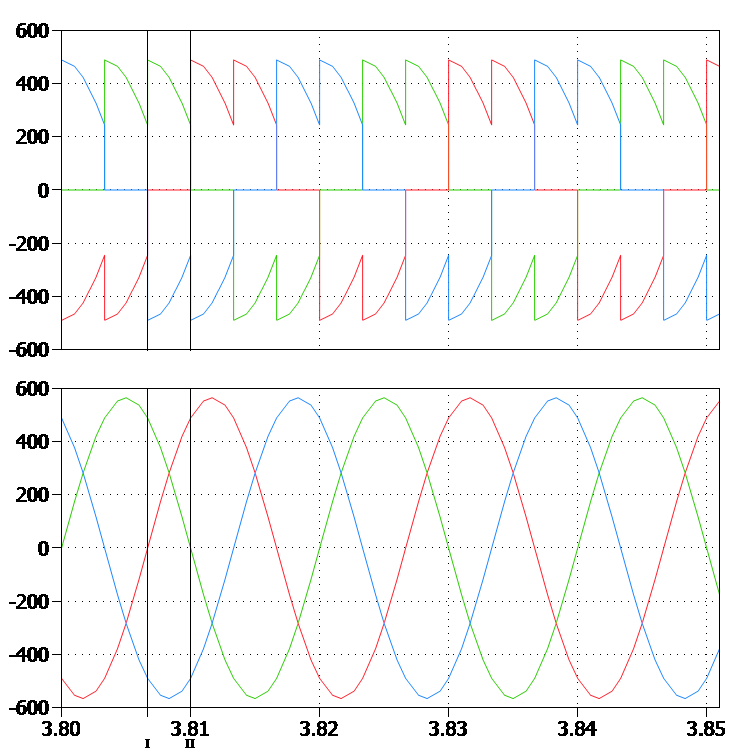
\includegraphics[width=0.45\linewidth]{3_phasiges_Phasenanschnit_60_Signal.png}\label{fig:3_phasiges_Phasenanschnitt_60_Signal}}\qquad
	\subfloat[][]{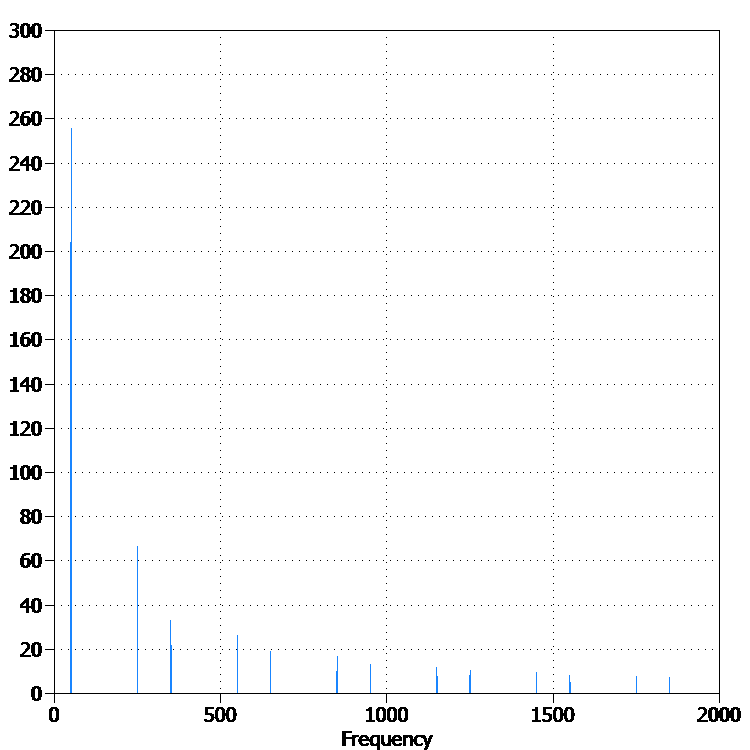
\includegraphics[width=0.45\linewidth]{3_phasiges_Phasenanschnit_60_FFT.png}\label{fig:3_phasiges_Phasenanschnitt_60_FTT}}
	\caption{Dreiphasige Phasenanschnittsteuerung mit 60\textdegree (a) Signal (b) FFT}
	\label{fig:dreiphasige_Phasenanschnittsteuerung_mit_60}
\end{figure}


\begin{figure}[ht!]
	\centering
	\subfloat[][]{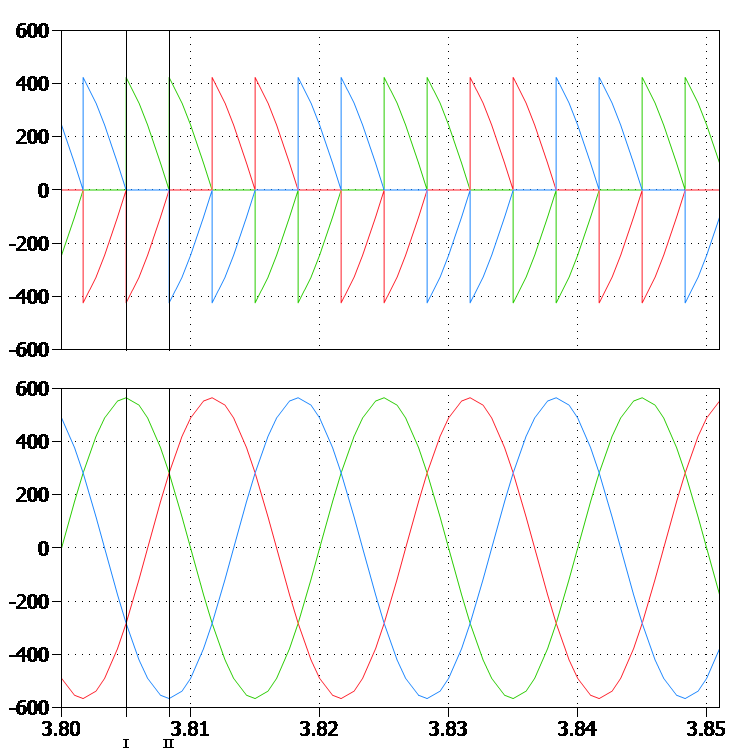
\includegraphics[width=0.45\linewidth]{3_phasiges_Phasenanschnit_90_Signal.png}\label{fig:3_phasiges_Phasenanschnitt_90_Signal}}\qquad
	\subfloat[][]{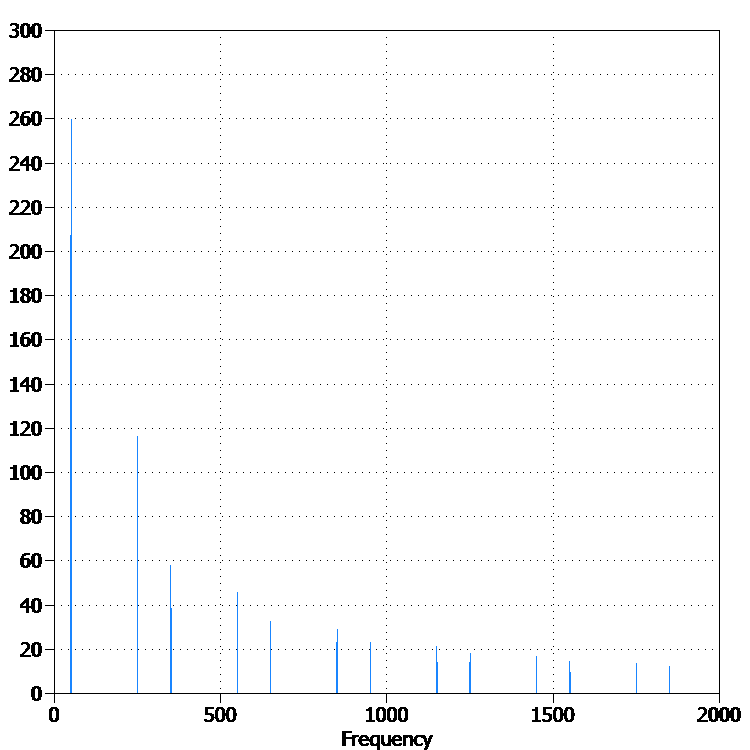
\includegraphics[width=0.45\linewidth]{3_phasiges_Phasenanschnit_90_FFT.png}\label{fig:3_phasiges_Phasenanschnitt_90_FTT}}
	\caption{Dreiphasige Phasenanschnittsteuerung mit 90\textdegree (a) Signal (b) FFT}
	\label{fig:dreiphasige_Phasenanschnittsteuerung_mit_90}
\end{figure}
Anhand von Cursor \RomanNumeralCaps{1} erkennt man, dass zuerst eine positive Halbwelle der Eingangsspannung, des ersten Phase (grün), anliegt. Der positive Thyristor des ersten Triacs zündet bei 90\textdegree, beziehungsweise bei 60\textdegree\hspace{0.02cm}. Da der Sternpunkt bei dieser Schaltung nicht mit dem Neutralleiter verbunden ist, tritt eine negative Spannung über dem Thyristor des zweiten Triac auf (rot). Beim Cursor \RomanNumeralCaps{2} hat es eine negative Eingangsspannung der zweiten Phase (blau). Somit zündet der negative Thyristor des dritten Triacs, und die entgegengesetzte positive Spannung entsteht über dem ersten Thyristor (grün) des ersten Triacs. Diese Abfolge wird beliebig weitergeführt. Da es sich um eine ohmsche Last handelt, verhält sich das Stromsignal phasengleich wie die Spannungskurve. Auf der Abbildung \ref{fig:3_phasiges_Phasenanschnitt_60_FTT} und \ref{fig:3_phasiges_Phasenanschnitt_90_FTT} erkennt man die beiden  FFTs der jeweiligen Phasenanschnittsteuerungen. Es ist ersichtlich, dass auch bei dreiphasigen Phasenanschnittsteuerungen nur harmonische Oberschwingungen vorkommen und keine Sub- oder Zwischenharmonische. 

\newpage

\subsubsection{Dreiphasige Schwingungspaketsteuerung mit Duty Cycles von 0.5 und 0.8}\label{sec:Schwingungspaketsteuerung_Simulation}
Nachfolgend sind die dreiphasigen Schwingungspaketsteuerungen mit den Duty Cycle von 0.5 in Abbildung \ref{fig:3_phasiges_Schwingungspaket_Signal_0_5} und 0.8 in Abbildung \ref{fig:3_phasiges_Schwingungspaket_Signal_0_8} dargestellt. Die drei Eingangsspannungen und die Widerstände richtete man gleich, wie bei der dreiphasigen Phasenanschnittsteuerung, ein. Daher sind auch die Strom- und Spannungsverläufe wieder phasengleich. Bei den grünen, roten und blauen Signale handelt es sich um die Spannungspakete über den einzelnen Widerständen.\\
In den Bildern \ref{fig:3_phasiges_Schwingungspaket_FTT_0_5} und \ref{fig:3_phasiges_Schwingungspaket_FTT_0_8} sind die FFTs der Schwingungspaketsteuerung ersichtlich. Man erkennt vor allem, dass es vor und nach 50 Hz (hoher Peak) viele sub- und zwischenharmonische Oberschwingungen hat. Eine gewisse Ähnlichkeit mit den einphasigen Paketsteuerungen ist ersichtlich.
 

\begin{figure}[ht!]
	\centering
	\subfloat[][]{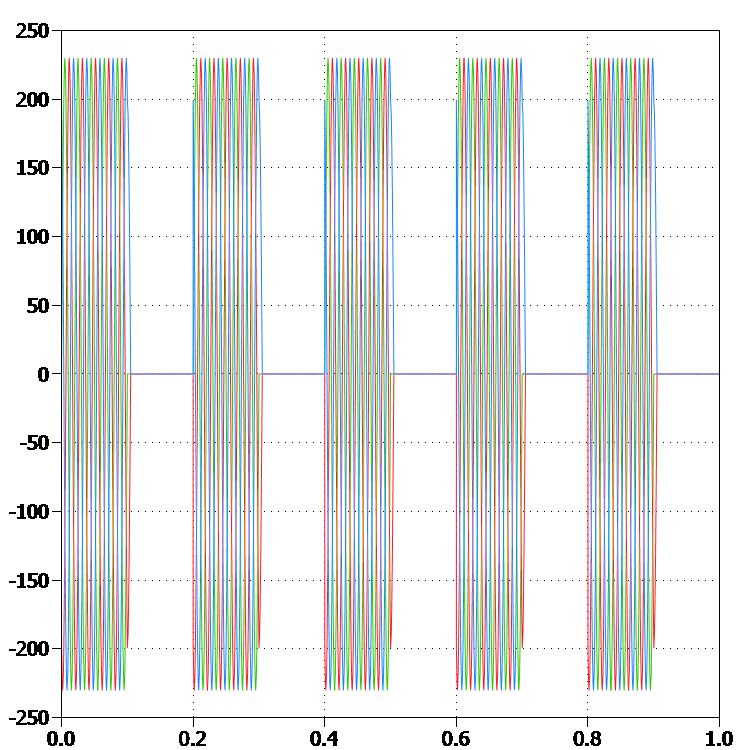
\includegraphics[width=0.45\linewidth]{3_phasiges_Schwingungspaket_Signal_0_5.png}\label{fig:3_phasiges_Schwingungspaket_Signal_0_5}}\qquad
	\subfloat[][]{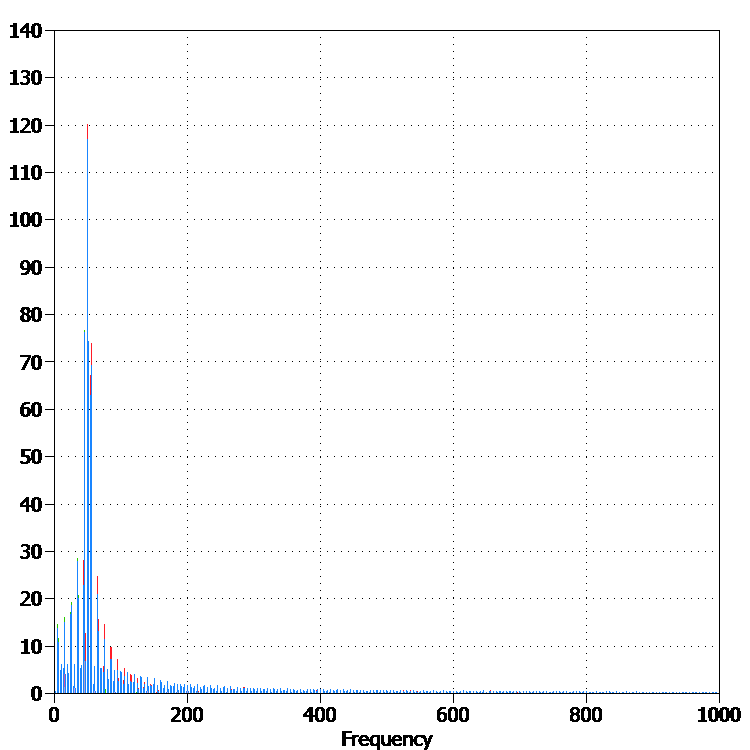
\includegraphics[width=0.45\linewidth]{3_phasiges_Schwingungspaket_FTT_0_5.png}\label{fig:3_phasiges_Schwingungspaket_FTT_0_5}}
	\caption{Dreiphasige Schwingungspaketsteuerung mit Duty Cycle 0.5 (a) Signal (b) FFT}
	\label{fig:3_phasiges_Schwingungspaket_0_5}
\end{figure}



\begin{figure}[ht!]
	\centering
	\subfloat[][]{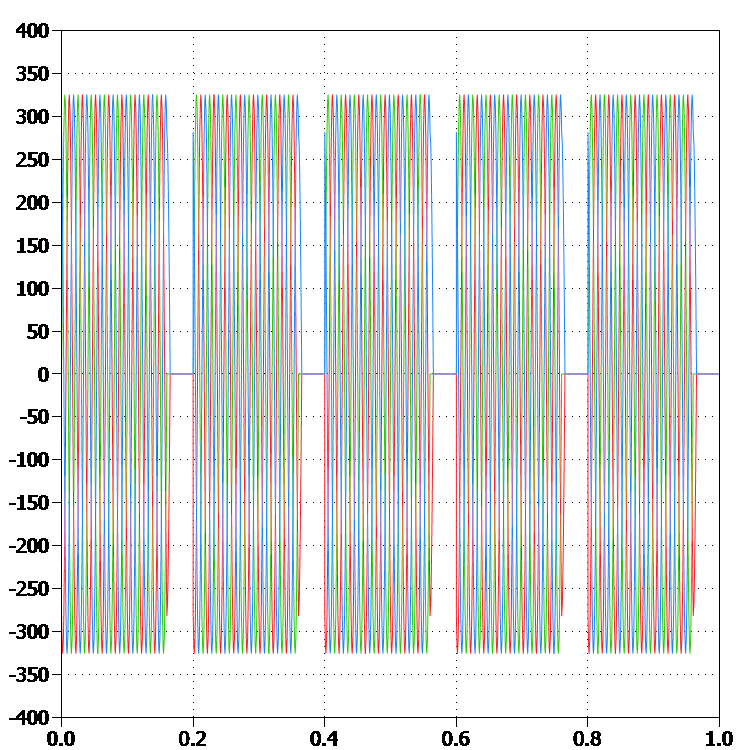
\includegraphics[width=0.45\linewidth]{3_phasiges_Schwingungspaket_Signal_0_8.png}\label{fig:3_phasiges_Schwingungspaket_Signal_0_8}}\qquad
	\subfloat[][]{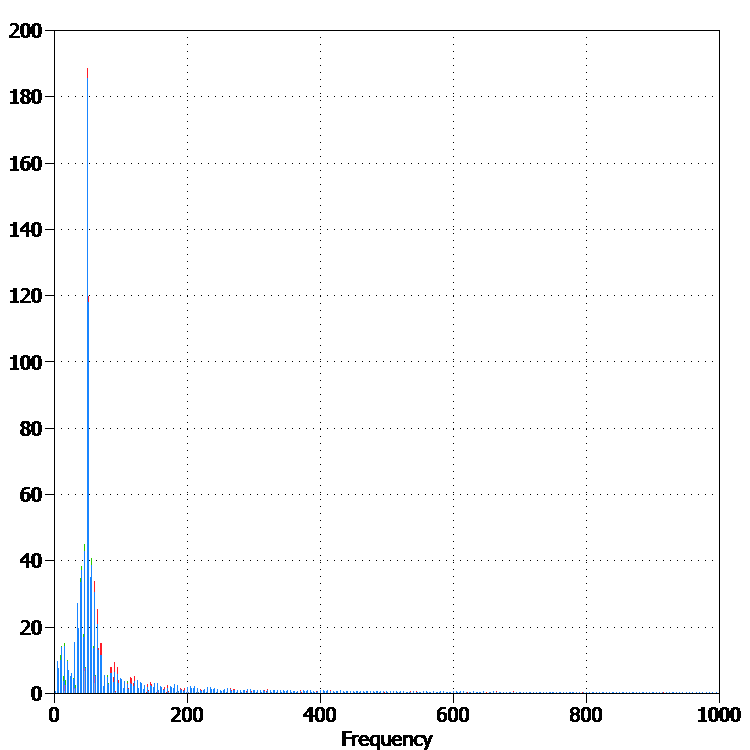
\includegraphics[width=0.45\linewidth]{3_phasiges_Schwingungspaket_FTT_0_8.png}\label{fig:3_phasiges_Schwingungspaket_FTT_0_8}}
	\caption{Dreiphasige Schwingungspaketsteuerung mit Duty Cycle 0.8 (a) Signal (b) FFT}
	\label{fig:3_phasiges_Schwingungspaket_0_8}
\end{figure}

\newpage
\subsubsection{Einphasige Kombination des Auf- und Absteuerns}

Nach den Simulationen der beiden Steuerungsverfahren im ein- und dreiphasigen System wird die Kombination der beiden Verfahren entwickelt. In der Abbildung \ref{fig:1_phasig_sanftanlaser_Eingangssignal_Ausschnitt} erkennt man ein sanftes Ansteigen der Spannung bis auf die volle Leistung und nach einiger Zeit wieder ein sanftes Herunterfahren der Spannung, bis sie null beträgt. In Abbildung \ref{fig:1_phasig_sanftanlaser_Eingangssignal_duty_cycle_0.5} ist der Duty Cycle auf 0.5 eingestellt. Die einzelnen Pakete verhalten sich nun so wie das sanfte Hoch- und Runterfahren der Spannung, erkennbar in Abbildung \ref{fig:1_phasig_sanftanlaser_Eingangssignal_Ausschnitt}. Vergleicht man das FFT in Abbildung \ref{fig:1_phasig_sanftanlaser_FFT} mit dem FFT des Schwingungspaketes mit hartem Zu- und Wegschalten \ref{fig:plecs_Schwingungspaket_0_5_1000} ist eine Verringerung der subharmonischen Schwingungen ersichtlich. Das sanfte Hinauf- und Hinunterfahren hat aber zufolge, dass die Oberwellen bei den Harmonischen zunehmen. 

\begin{figure}[ht!]
	\centering
	\subfloat[][]{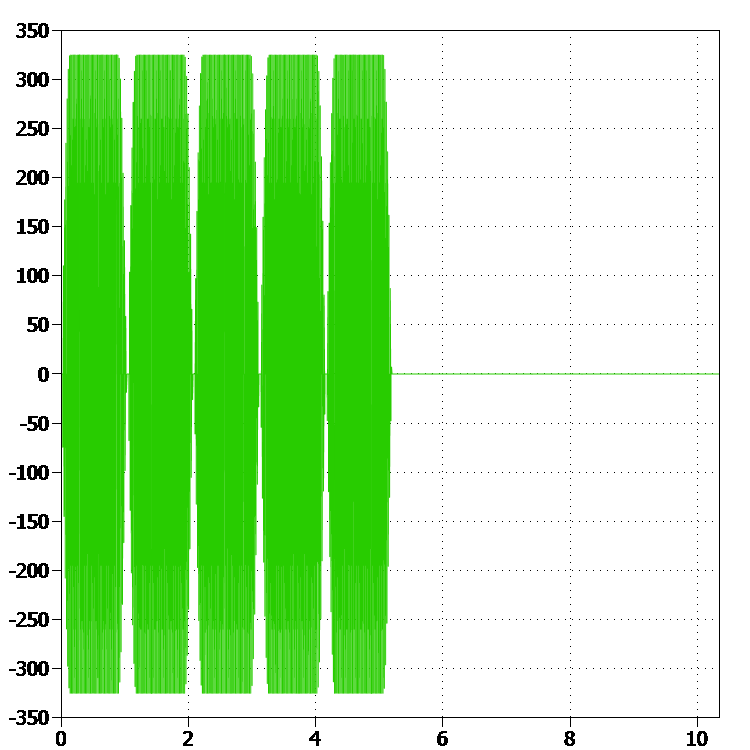
\includegraphics[width=0.43\linewidth]{1_phasig_sanftanlaser_Eingangssignal_duty_cycle_0_5.png}\label{fig:1_phasig_sanftanlaser_Eingangssignal_duty_cycle_0.5}}\qquad
	\subfloat[][]{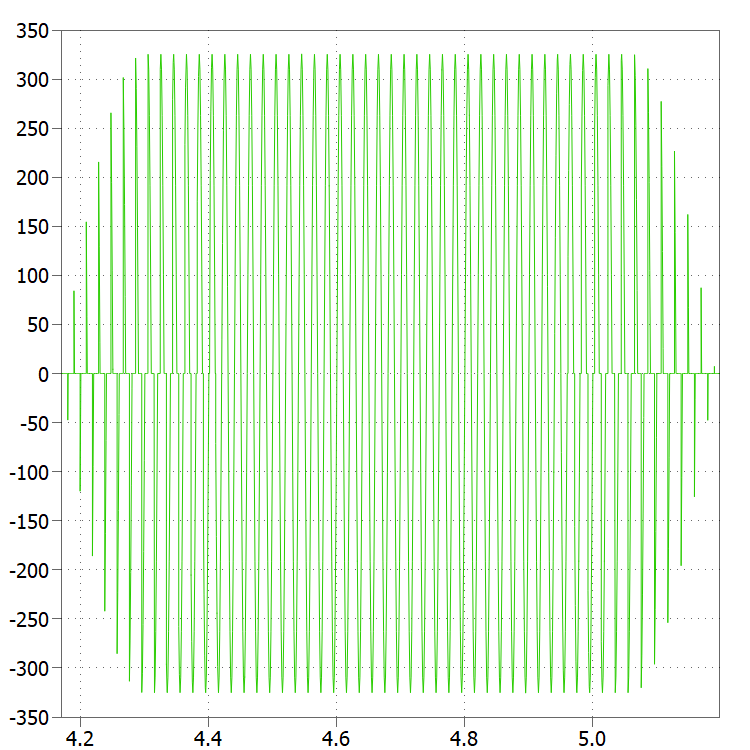
\includegraphics[width=0.43\linewidth]{1_phasig_sanftanlaser_Eingangssignal_Ausschnitt.png}\label{fig:1_phasig_sanftanlaser_Eingangssignal_Ausschnitt}}
	\caption{Einphasiges Hoch- und Runterfahren mit einem Duty Cycle von 0.5 (a) Eingangssignal (b) Ausschnitt eines Paketes}
	\label{fig:einphasiges_Sanft_anlassen_Einganssignal}
\end{figure}

\begin{figure}[ht!]
	\centering
	\subfloat[][]{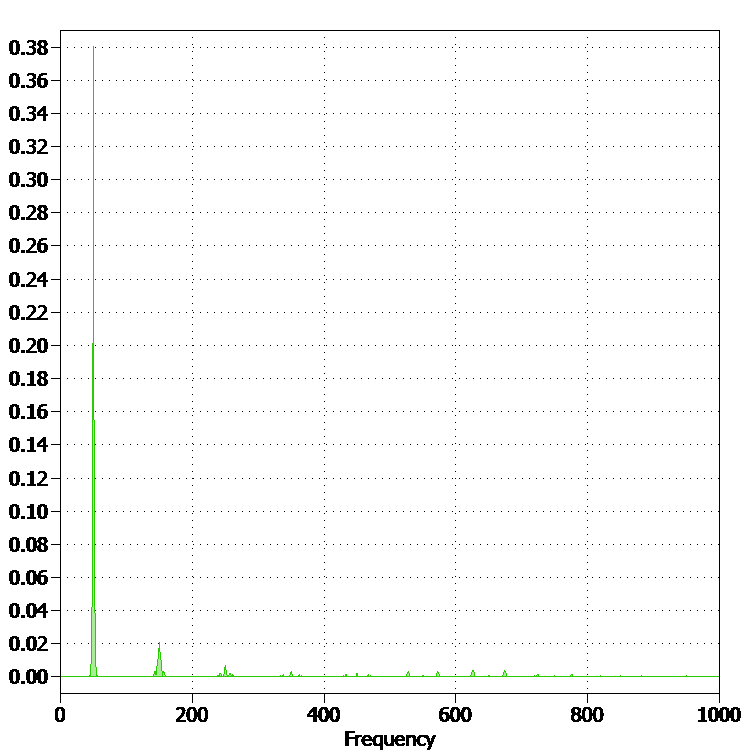
\includegraphics[width=0.43\linewidth]{1_phasig_sanftanlaser_FFT.png}\label{fig:1_phasig_sanftanlaser_FFT}}\qquad
	\subfloat[][]{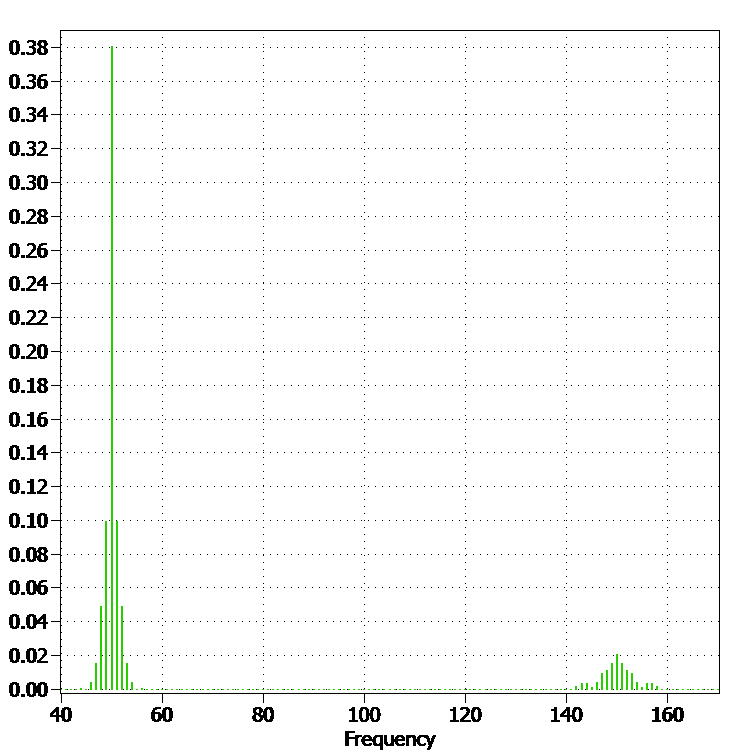
\includegraphics[width=0.43\linewidth]{1_phasig_sanftanlaser_FFT_Ausschnitt.png}\label{fig:1_phasig_sanftanlaser_FFT_Ausschnitt}}
	\caption{FTT des einphasigen Hoch- und Runterfahrens mit einem Duty Cycle von 0.5 (a) 0 - 2000 Hz (b) Ausschnitt 40 - 170 Hz}
	\label{fig:einphasiges_Sanft_anlassen_FTT}
\end{figure}

\newpage
\subsubsection{Dreiphasige Kombination des sanften Auf- und Absteuerns}

Die Abbildung \ref{fig:drei_phasiges_Sanft_anlassen} zeigt eine dreiphasige Steuerung des Hoch- und Runterfahrens. Das dargestellte Spannungssignal hat einen Duty Cycle von 0.5, ersichtlich in Abbildung \ref{fig:3_phasig_sanftanlaser_Eingangssignal_duty_cycle_0_5}. Die Kurve und die Funktion der Spannung verhalten sich ähnlich wie die Kombination des einphasigen Hoch- und Runterfahrens. Die drei Farben Grün, Rot und Blau zeigen die verschiedenen Spannungen über den drei Widerständen an. Da es sich hier um eine rein ohmsche Last handelt, sind die Ströme phasengleich mit den Spannungen. Beim FFT in Abbildung \ref{fig:dreiphasiges_Sanft_anlassen_FTT} von 0 - \SI{2000}{Hz} erkennt man den grössten Peak bei der Grundschwingung von \SI{50}{Hz}. Die sub- und zwischenharmonischen Schwingungen fallen bei der sanften Auf- und Absteuerung viel mehr ins Gewicht als die Harmonischen. Sie sind nur noch minimal vorhanden.   


\begin{figure}[ht!]
	\centering
	\subfloat[][]{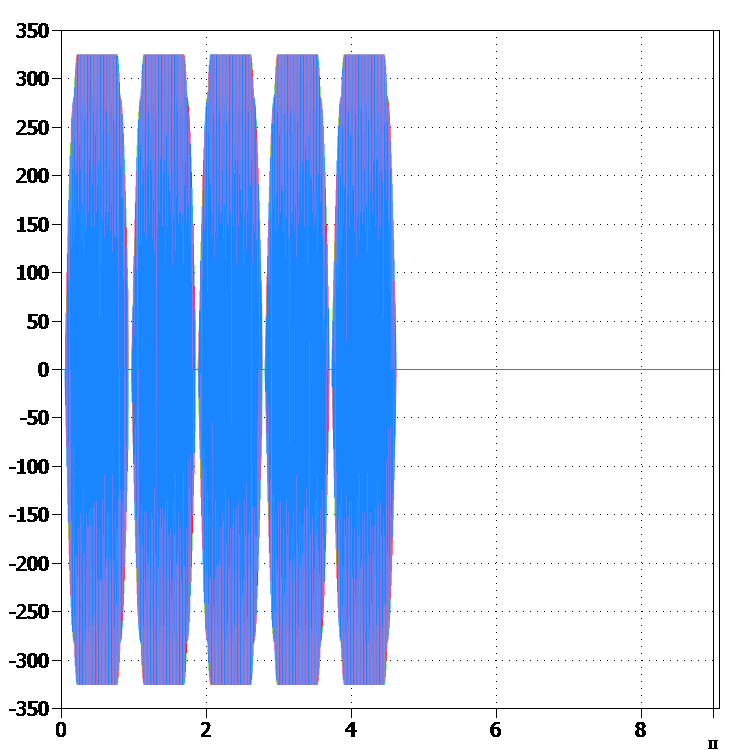
\includegraphics[width=0.43\linewidth]{3_phasig_sanftanlaser_Eingangssignal_duty_cycle_0_5.png}\label{fig:3_phasig_sanftanlaser_Eingangssignal_duty_cycle_0_5}}\qquad
	\subfloat[][]{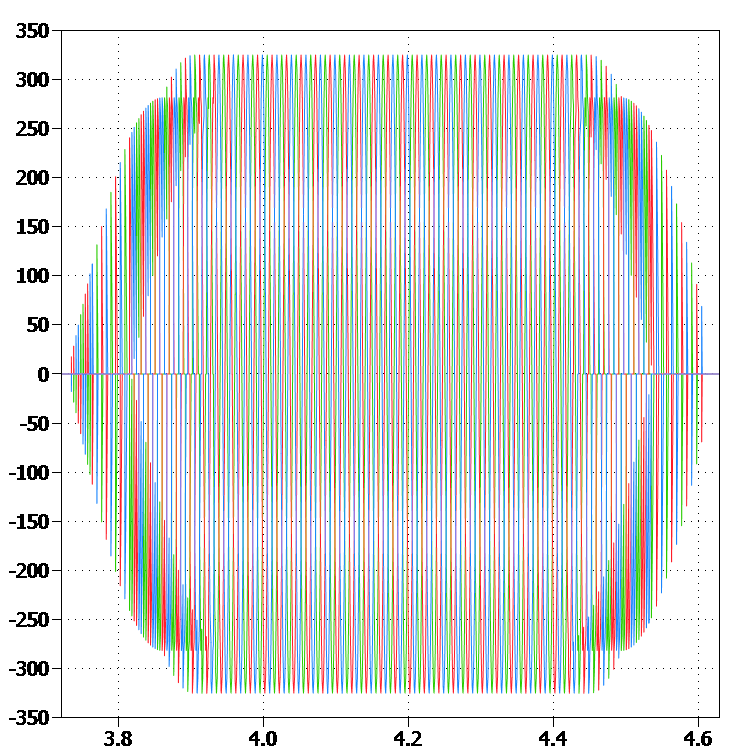
\includegraphics[width=0.43\linewidth]{3_phasig_sanftanlaser_Eingangssignal_Ausschnitt_0_5.png}\label{fig:3_phasig_sanftanlaser_Eingangssignal_Ausschnitt_0_5}}
	\caption{Dreiphasiges Auf- und Absteuern mit einem Duty Cycle von 0.5 (a) Eingangssignal (b) Ausschnitt}
	\label{fig:drei_phasiges_Sanft_anlassen}
\end{figure}

\begin{figure}[ht!]
	\centering
	\subfloat[][]{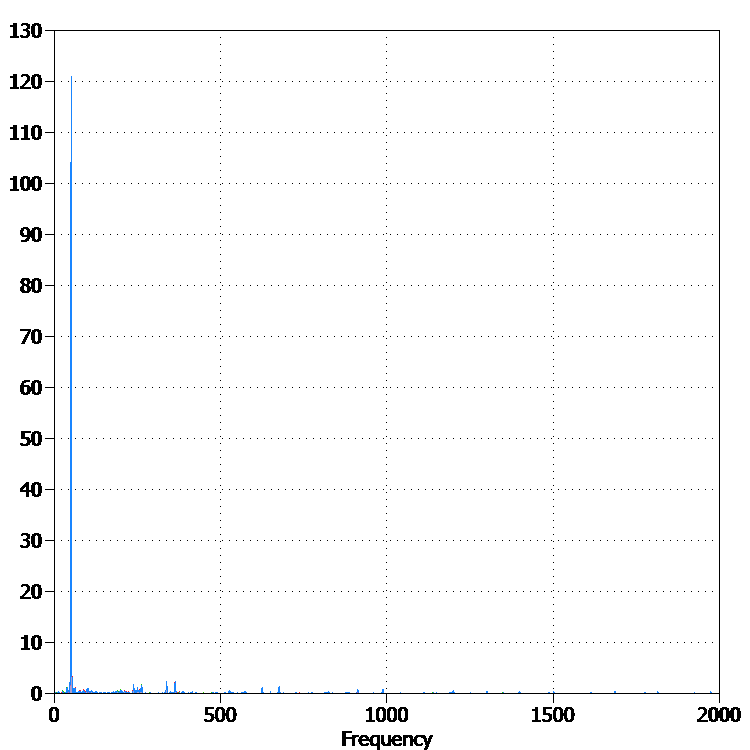
\includegraphics[width=0.43\linewidth]{3_phasig_sanftanlaser_FFT_0_5.png}\label{fig:3_phasig_sanftanlaser_FFT_0_5}}\qquad
	\subfloat[][]{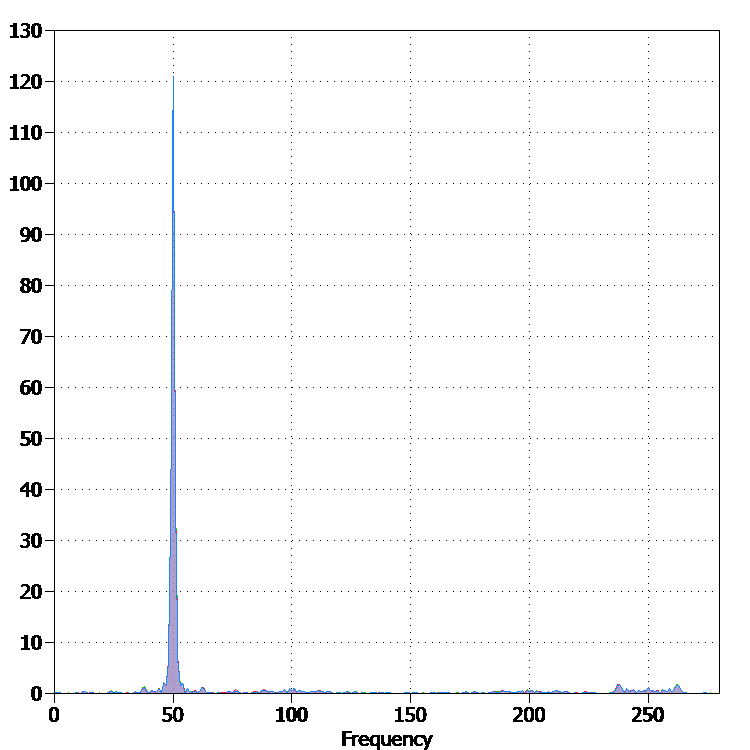
\includegraphics[width=0.43\linewidth]{3_phasig_sanftanlaser_FFT_Ausschnitt_0_5.png}\label{fig:3_phasig_sanftanlaser_FFT_Ausschnitt_0_5}}
	\caption{FTT des dreiphasigen Hoch- und Runterfahrens mit einem Duty Cycle von 0.5 (a) 0 - 2000 Hz (b) Ausschnitt 0 - 300 Hz}
	\label{fig:dreiphasiges_Sanft_anlassen_FTT}
\end{figure}

\newpage


\subsubsection{Alternative Ansteuerungen}\label{Spar-Ansteuerung}
In der Praxis kommen zum Teil die sogenannten Sparsteuerungen zum Einsatz. Bei dieser Steuerungsart werden nicht alle drei Phasen angesteuert, sondern nur eine oder zwei. Damit man ein solches Verfahren erhält, überbrückt man die Thyristoren in der gewünschten Phase. Eine weitere Möglichkeit ist, die Thyristoren gar nicht erst in die Schaltung einzubinden. Man kann sie deshalb kurzerhand weglassen. Die überbrückte Phase dient dabei als Ausgleichs- und Rückleiter. Mit Plecs wurden solche Verfahren simuliert, wobei die Last in Stern oder Dreieck geschaltet ist. Die Ansteuerungen der nicht veränderten Phasen verhält sich gleich wie die der dreiphasigen Kombinationssteuerung. Das folgende Kapitel \ref{sec:2_phasen_Ansteuerung} zeigt die Simulation einer Zwei-Phasen-Ansteuerung, bei der die Last in Stern geschaltet ist. Die einphasige Ansteuerung befindet sich im Anhang im Kapitel \ref{sec:Sparvariante_1Thyristor}.




%In der Praxis werden nicht immer alle 3 Phasen angesteuert, sogenannte Sparansteuerungen. Dabei können nur zwei oder auch nur eine Phase angesteuert werden. Das heisst, dass zum Beispiel bei der Zwei-Phasen-Ansteuerung bei einer Phase der Thyristor überbrückt wird beziehungsweise der Thyristor gar nicht vorhanden ist. Dabei dient die überbrückte Phase als Ausgleichs- und Rückleiter. Diese Fälle wurden mit Plecs simuliert wobei die Last in Stern und in Dreieck geschaltet werden kann. Wie bei der 3-Phasen Ansteuerung, wurde für die alternativen Ansteuerung auch der Sanft-Anlass, die Kombination mit Phasenanschnitts- und Schwingungspaketsteuerung, simuliert.

\subsubsection*{Zwei-Phasen-Ansteuerung mit Last in Stern}\label{sec:2_phasen_Ansteuerung}
Bei der Abbildung \ref{fig:2_phasige_ansteuerung_mit_Last} erkennt man eine zweiphasige Ansteuerungsart, bei der die dritte Phase (blau) überbrückt wurde. Es sind wiederum fünf Schwingungspakete ein- und ausgeschaltet, was einem Duty Cycle von 0.5 entspricht. In Abbildung \ref{fig:2_phasige_ansteuerung_mit_Last_ausschnitt_Einganssignal} ist eines der fünf Schwingungspakete dargestellt. Es ist ersichtlich, dass die Spannung, welche über die Thyristoren anfällt, immer direkt über die überbrückte Phase abfällt. Daher sind am Anfang und Ende die blauen Spannungspeaks ersichtlich. Sobald jedoch die volle Spannung bezogen wird, verhält sich dieses Verfahren wie die dreiphasige Kombination der sanften Ansteuerung. Alle Thyristoren haben daher einen Zündwinkel von 0\textdegree\hspace{0.02cm} und das System verhält sich symmetrisch.\\
In der Abbildung \ref{fig:2_phasige_ansteuerung_mit_Last_FFT} ist das FFT der Zwei-Phasen-Ansteuerung, wiederum von 0 bis \SI{2000}{Hz} auf der linken Seite und 0 bis \SI{280}{Hz} auf der rechten Seite dargestellt. Vergleicht man dies, mit dem der dreiphasigen Kombination, erkennt man, dass die Ausprägung der Oberschwingungen bei diesem Verfahren viel grösser ist. Ausserdem ist bei \SI{150}{Hz}, der dritten Harmonischen, ein Spannungspeak erkennbar. Dieser kommt davon, dass eine Asymmetrie zwischen den drei Phasen herrscht, da die dritte Phase nicht angesteuert wird.

\begin{figure}[ht!]
	\centering
	\subfloat[][]{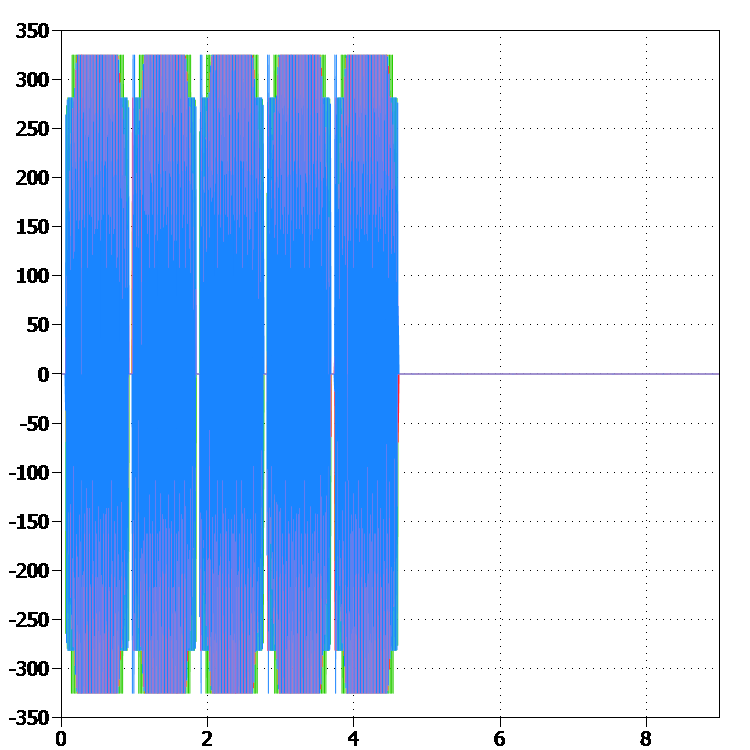
\includegraphics[width=0.43\linewidth]{2_phasige_ansteuerung_mit_Last_gesamtes_Einganssignal.png}\label{fig:2_phasige_ansteuerung_mit_Last_gesamtes_Einganssignal}}\qquad
	\subfloat[][]{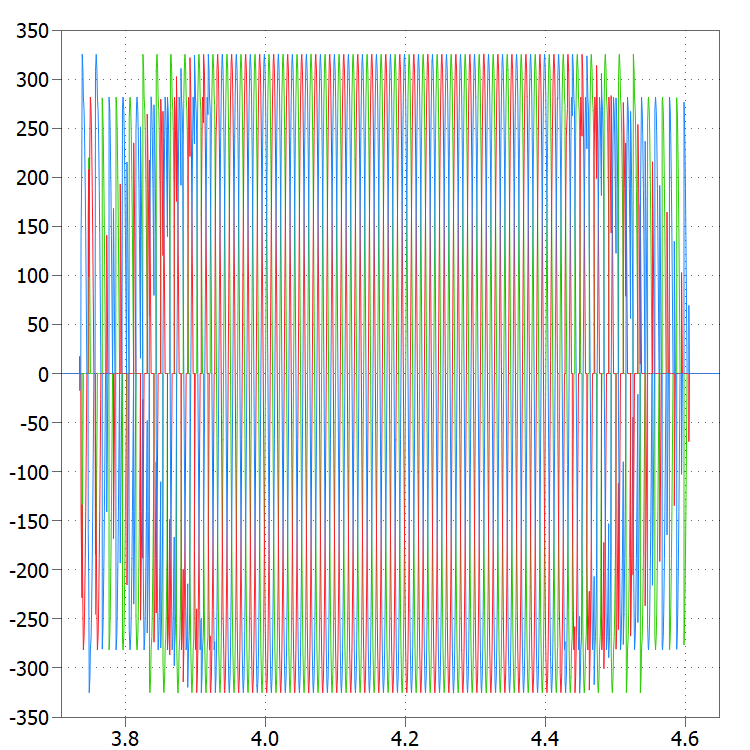
\includegraphics[width=0.43\linewidth]{2_phasige_ansteuerung_mit_Last_ausschnitt_Einganssignal.png}\label{fig:2_phasige_ansteuerung_mit_Last_ausschnitt_Einganssignal}}
	\caption{Zweiphasige Ansteuerung mit Last in Stern (a) Eingangssignal (b) Ausschnitt}
	\label{fig:2_phasige_ansteuerung_mit_Last}
\end{figure}


\begin{figure}[ht!]
	\centering
	\subfloat[][]{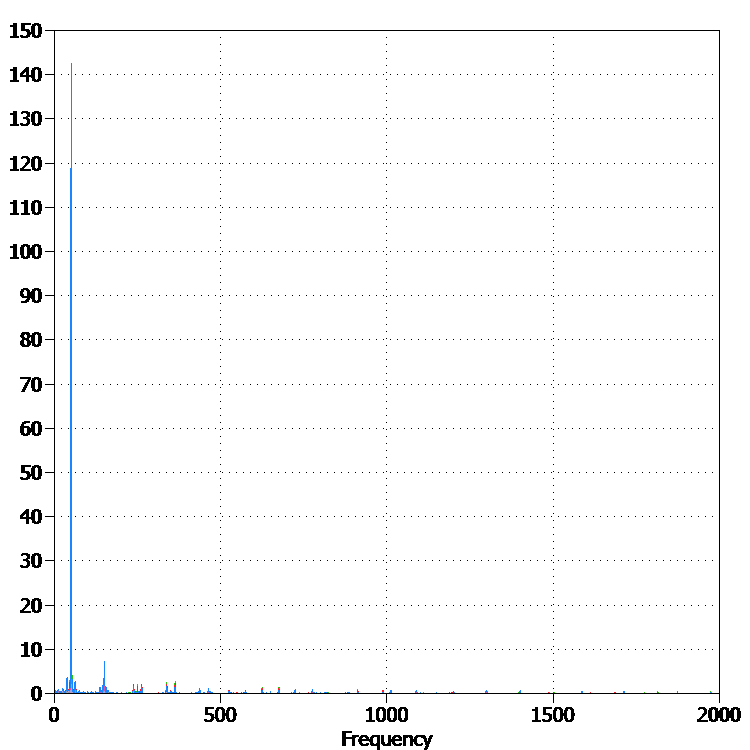
\includegraphics[width=0.43\linewidth]{2_phasige_ansteuerung_mit_Last_FFT_Komplet.png}\label{fig:2_phasige_ansteuerung_mit_Last_FFT_Komplet}}\qquad
	\subfloat[][]{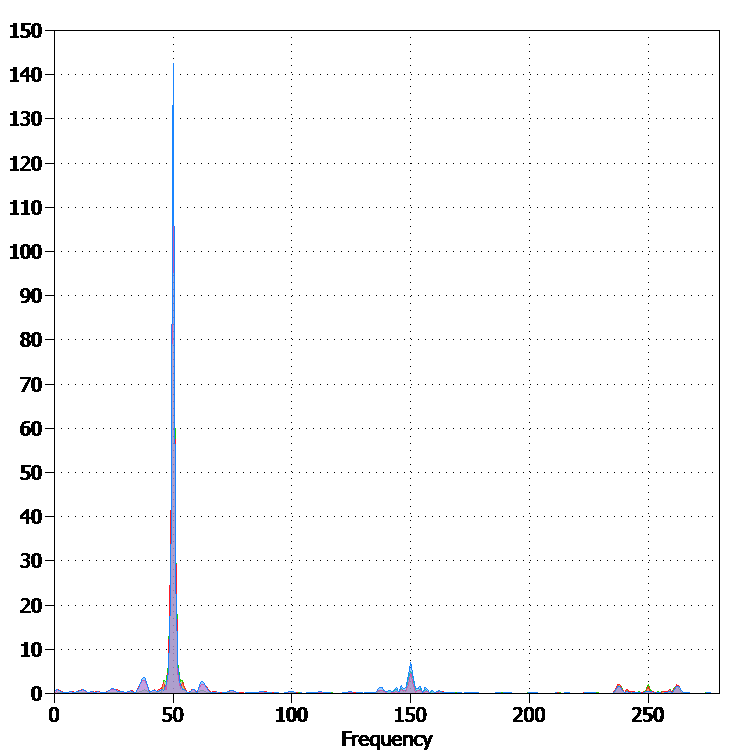
\includegraphics[width=0.43\linewidth]{2_phasige_ansteuerung_mit_Last_FFT_Ausschnitt.png}\label{fig:2_phasige_ansteuerung_mit_Last_FFT_Ausschnitt}}
	\caption{FTT der zweiphasigen Ansteuerung  (a) 0 - 2000 Hz (b) Ausschnitt 0 - 280 Hz}
	\label{fig:2_phasige_ansteuerung_mit_Last_FFT}
\end{figure}



\newpage
\subsubsection*{Halbwellensteuerung}
Eine weitere Möglichkeit, die Thyristoren anzusteuern, ist die Halbwellensteuerung. Dabei wird die positive Halbwelle einer Phase und zwei negative Halbwellen der anderen Phasen auf die Last geführt. Dies ist mit dem Thyristorsteller, welcher für das Projekt benutzt wurde, nicht möglich, da dieser alle 3 Phasen gleich ansteuert. Deshalb wurde dieser Fall nur mit Plecs simuliert, siehe Abbildung \ref{fig:HalbwellensteuerungT}. Das Problem bei dieser Steuerung ist, dass, wenn der Sternpunkt nicht mit dem Nullpunkt verbunden wird, ist der Phasenverlauf im Plecs schwer zu kontrollieren. Da die Summe der Spannungen immer 0 geben muss und die Spannungen phasenverschoben sind, gibt es einen sehr unschönen Spannungsverlauf. Wenn das FFT analysiert wird, fällt schnell auf, das die Grundschwingung von \SI{50}{Hz} nicht den höchsten Peak hat.

\begin{figure}[ht!]
	\centering
	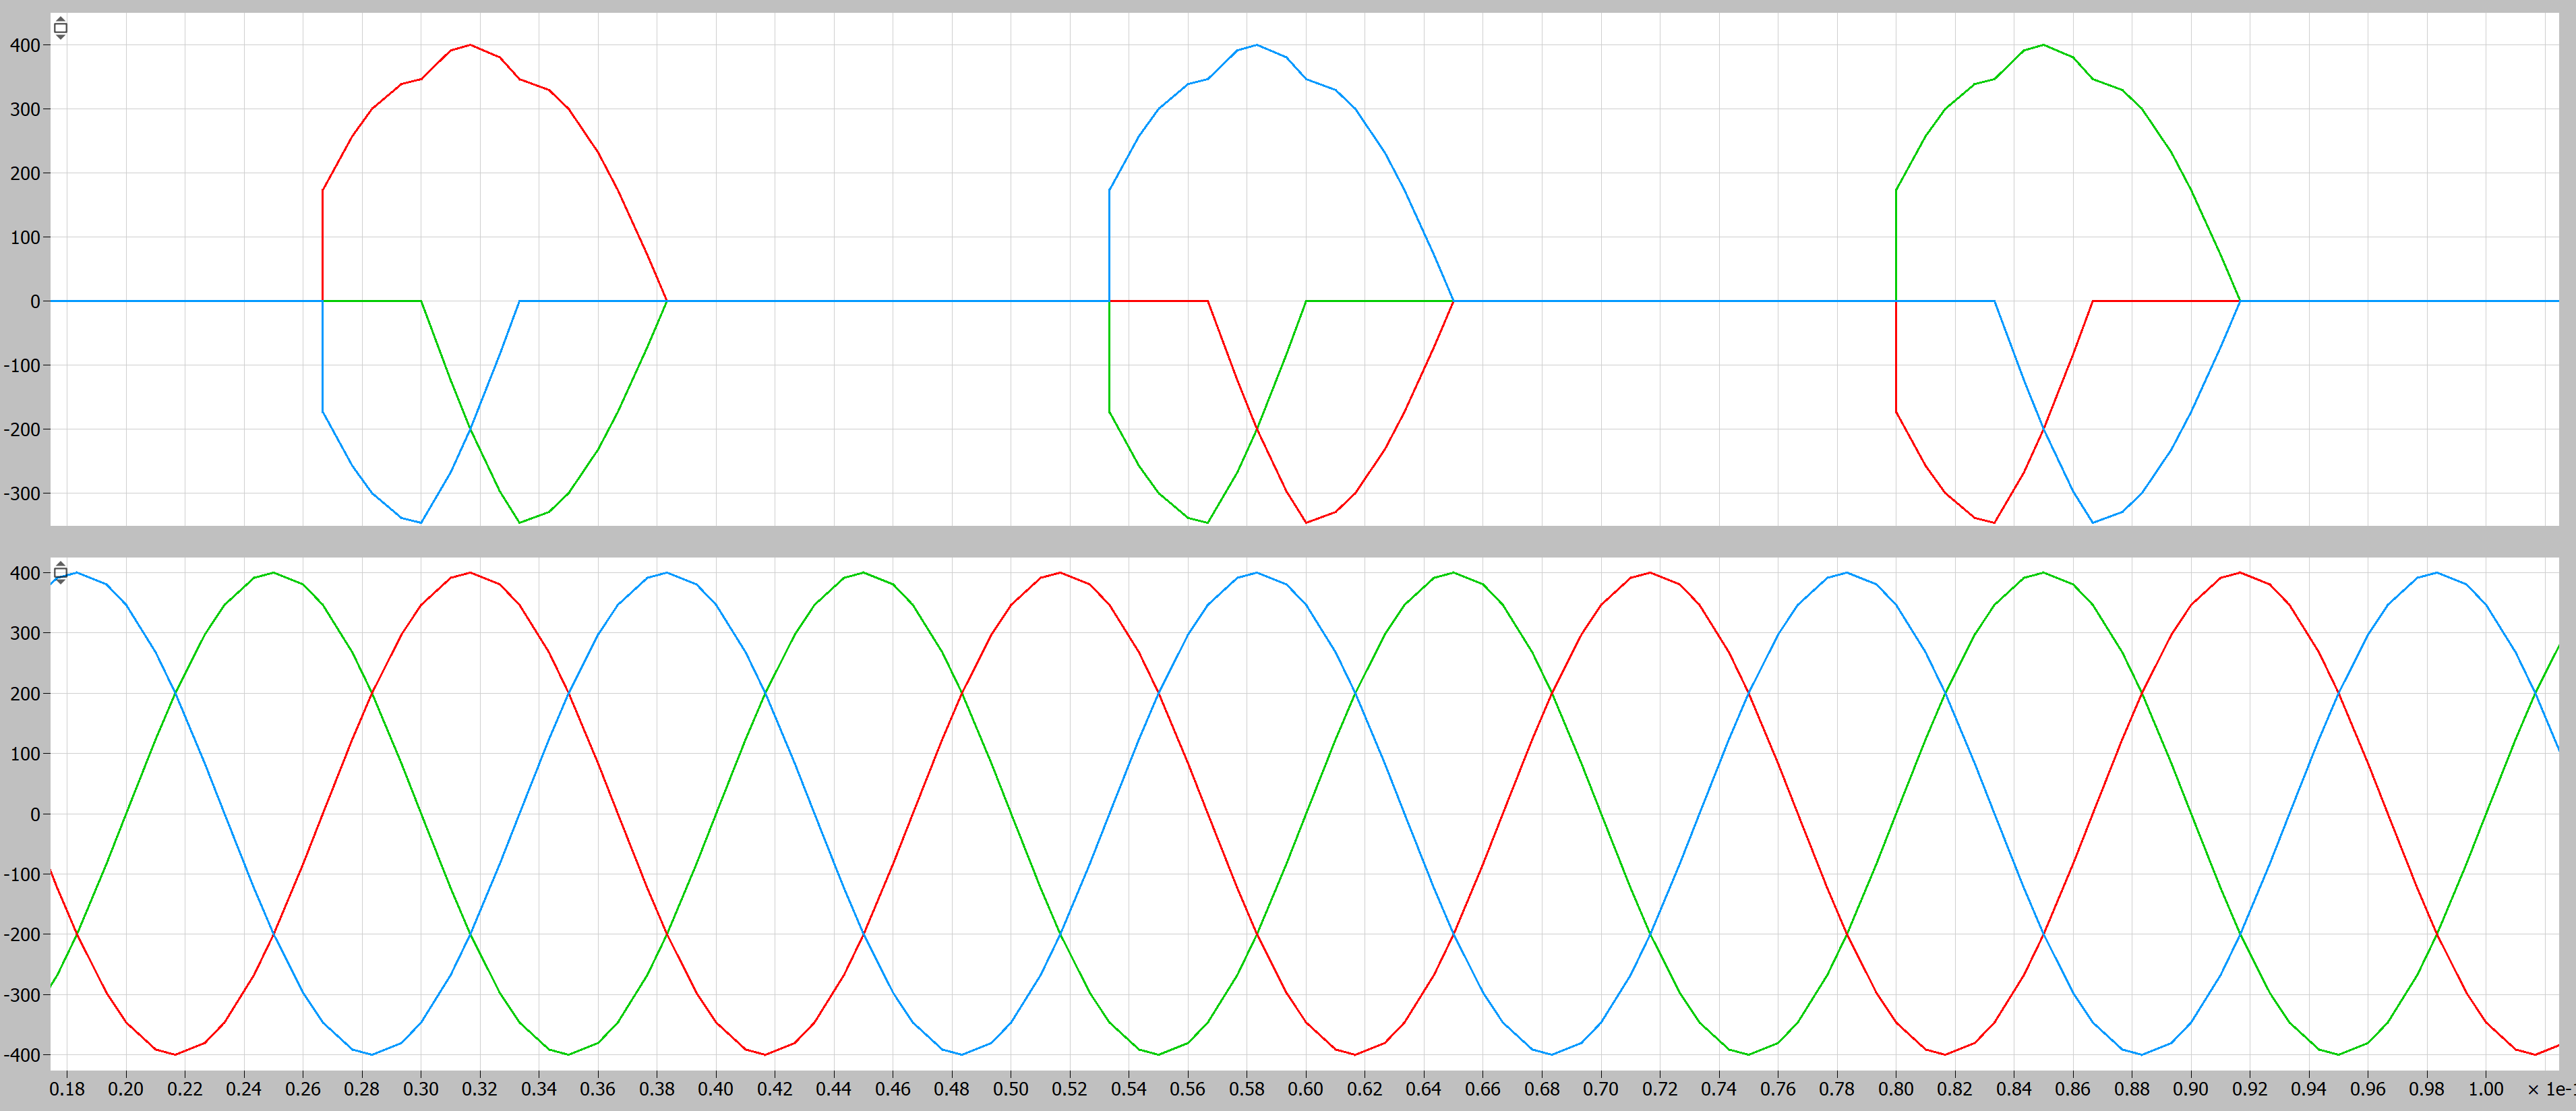
\includegraphics[width=\linewidth]{Halbwellensteuerung.png}
	\caption{Simulation mit der Halbwellensteuerung und das FFT}
	\label{fig:HalbwellensteuerungT}
\end{figure}

